\documentclass[twoside,a4paper,11pt]{report}

%*******************************************************
% From page 7 of Preparing and Submitting Your
% Thesis - A guide for MPhil and PhD students:
% The thesis submitted for examination shall be typewritten
% or printed on one side or both sides of International size
% A4 paper (except for drawings, maps or tables on
% which no restriction is placed), with a margin of
% not less than 35mm on both right and left-hand
% edges of each page.
% There is no stipulation for the top and bottom margins,
% but it is recommended that they should be 25mm.
% From page10:
% Font heights are usually measured in points and
% the most easily readable fonts are 10 point and 12 point.
%*******************************************************

\usepackage[left=37mm,right=37mm,top=27mm,bottom=27mm]{geometry}

%*******************************************************
% Include packages that you wish to use.
%*******************************************************

%\usepackage{tikz}
%\usetikzlibrary{shapes,arrows}
%\usepackage{multicol} % use multicolumn
%\usepackage{rotating} % to create a figure in landscape mode
%\usepackage{longtable} % this is for longtable
%\usepackage{array}
%\usepackage{amsthm}
%\usepackage{amsmath}

% For inserting graph
\usepackage{graphicx}

% For using website link
\usepackage{url}

% For cite more than two references
\usepackage{cite}

% For align equation
\usepackage{amsmath}

% This is for the List of Abbreviations
\usepackage{nomencl}
\makenomenclature

%*******************************************************
% Define hyphenation for some special words
%*******************************************************

\usepackage{hyphenat} % this define hyphenation, an example is given.
\hyphenation{electro-magnets}

%*******************************************************
% Make "clickable" Table of Contents
%*******************************************************
\usepackage{color}   %May be necessary if you want to color links
\usepackage{hyperref}
\hypersetup{
    colorlinks=true, %set true if you want colored links
    linktoc=all,     %set to all if you want both sections and subsections linked
    linkcolor=blue,  %choose some color, e.g. blue, if you want links to stand out
    }

%*******************************************************
% Set line spacing
%*******************************************************

% change it to 1 becomes single line spacing. Change it to 1.5 is a half line spacing.
\renewcommand{\baselinestretch}{1.5}

%*******************************************************
% This is the start of the thesis
%*******************************************************

\begin{document}

%*******************************************************
% From page 10 of Preparing and Submitting Your Thesis
% A guide for MPhil and PhD students:
% Modern word processing programs will automatically
% adjust the line spacing to match the size of text on any line.
% Single line spacing will produce a dense but readable
% text: the text may seem less formidable if one and a
% spacing is used. Double spacing results in a rather
% empty looking page and significantly increases
% the number of pages in a thesis.
%*******************************************************

%*******************************************************
% These are front matters.
% Abstract
% Title page
% Declaration
% Acknowledgment
% Table of Contents (Including List of Tables and List of Figures)
% List of Abbreviations
%*******************************************************

\pagenumbering{roman}
\pagestyle{plain}

%*******************************************************
% Abstract
%*******************************************************
\phantomsection
\addcontentsline{toc}{chapter}{Abstract}

\begin{center}

Abstract of thesis entitled\\

\bigskip

    \huge\textbf{Search for chargino and neutralino production in final states with two same-sign leptons, jets and missing transverse momentum at $\sqrt{s} = 13$ TeV with the ATLAS detector} \\

    \bigskip

    {\normalsize Submitted by}\\

\bigskip

    \Large{\textbf{Cheuk Yee LO}}\\

\bigskip

{\normalsize
for the degree of Doctor of Philosophy\\
at The University of Hong Kong\\
in November 2018\\}

\end{center}

\bigskip

The Standard Model in particle physics has successfully explained almost all experimental results in the microscopic scale with high accuracy.
However, the nature of dark matter and the Higgs mass hierarchy problem are still unanswered questions.
Supersymmetry (SUSY), which proposes a new symmetry between fermions and bosons, is one of the most promising theories beyond the Standard Model for potentially answering these questions.
In recent searches for supersymmetric particles that are involved in strong interaction, their masses were found to be above 1 TeV.
Since the production cross section drops as the masses of particles increase,
this might suggest that the pair production of electroweak gauginos, which tend to have lower mass, is a dominant SUSY production process at the Large Hadron Collider (LHC).
In addition, the upgrade in the increased center-of-mass energy of the proton-proton collisions $\sqrt{s}$ to 13 TeV has opened a new phase of exploration for electroweak SUSY productions.

In this thesis, a search is presented for the electroweak pair production of a chargino and a neutralino ($p + p \rightarrow \tilde{\chi}_1^\pm + \tilde{\chi}_2^0$),
where the chargino decays to the lightest neutralino and a W boson ($\tilde{\chi}_1^\pm \rightarrow \tilde{\chi}_1^0 + W$),
and the second lightest neutralino decays to the lightest neutralino and a Standard-Model-like Higgs boson ($\tilde{\chi}_2^0 \rightarrow \tilde{\chi}_1^0 + h$).
The final state with two same-sign leptons, jets and missing transverse momentum is considered in this search.
The two leptons come from the leptonic decay of the W boson and the Higgs boson, with the decay modes of  $h \rightarrow WW$, $h \rightarrow \tau \tau$ or $h \rightarrow ZZ$.
This analysis is based on the proton-proton collision data delivered by the LHC at $\sqrt{s}$ = 13 TeV with the ATLAS (A Toroidal LHC ApparatuS) particle detector.
The integrated luminosity of data is 36.1 fb$^{-1}$.

As a result, observations are consistent with the Standard Model predictions, therefore new exclusion limits for the masses of $\tilde{\chi}_1^\pm$/$\tilde{\chi}_2^0$ and $\tilde{\chi}_1^0$ are set, which supersedes the run 1 results.

\bigskip

\begin{center}

\rule{6cm}{0.025cm}\\
{\slshape An abstract of exactly 307 words}

\end{center}

%*******************************************************
% Titlepage
%*******************************************************
\phantomsection
\addcontentsline{toc}{chapter}{Title Page}

\begin{titlepage}
    \begin{center}
        \large
            \hfill
            \vfill
        \begingroup
            \huge\textsc{\textbf{This is the title of my thesis}} \\
            \bigskip
        \endgroup
        by\\
    \bigskip
        \Large\textsc{\textbf{Cheuk Yee LO}}\\
        \vfill
        \vfill
        \vfill
    {\normalsize
    A thesis submitted in partial fulfilment of the requirements for\\
    the Degree of Doctor of Philosophy\\
    at The University of Hong Kong.\\
        \bigskip
    August 2018}
        \vfill
        \end{center}
\end{titlepage}

%*******************************************************
% Declaration
%*******************************************************

\addcontentsline{toc}{chapter}{Declaration}

\chapter*{Declarations}

I declare that this thesis represents my own work, except where due acknowledgement is made, and that it has not been previously included in a thesis, dissertation or report submitted to this University or to any other institution for a degree, diploma or other qualifications.% This is copied from the declaration statement from the Handbook.

\bigskip
\bigskip
\bigskip
\bigskip
\bigskip
\bigskip
\bigskip
\bigskip

\begin{flushright}
    \begin{tabular}{p{2cm} p{4cm}}
        Signed & \dotfill \\
           & \center Cheuk Yee LO\\
    \end{tabular}
\end{flushright}

\bigskip
\bigskip
\bigskip

%*******************************************************
% Acknowledgments
%*******************************************************

\addcontentsline{toc}{chapter}{Acknowledgments}
\chapter*{Acknowledgments}

I would like to take this opportunity to thank some people who helped me do the research.

I would like to thank my supervisor Dr. Tu Yanjun for giving me the opportunity to do the research, for her support on my research and for her guidance and suggestions on my analysis.

I would like to thank Dr. Zhang Dongliang.
He taught me almost everything on the analysis.
He taught me the linux software: the linux shell, the text editor (vim) and the revision control system (svn).
He taught me the ATLAS software: the event analysis software (ROOT and RootCore), the data acquisition software(dq2 and rucio) and the distributed computing management (grid and panda).
He taught me the typesetting system (latex).
He taught me the ALTAS detector: trigger system and GRL.
He also helped our group to write the multiLepSearch package to generate the ntuple.

I would like to thank Dr. Daniela Paredes.
She gave a lot of suggestions on my analysis.
She also helped our group to do analysis.



%*******************************************************
% This program is free software: you can redistribute it and/or modify
% it under the terms of the GNU General Public License as published by
% the Free Software Foundation, either version 3 of the License, or
% (at your option) any later version.
%
% This program is distributed in the hope that it will be useful,
% but WITHOUT ANY WARRANTY; without even the implied warranty of
% MERCHANTABILITY or FITNESS FOR A PARTICULAR PURPOSE.  See the
% GNU General Public License for more details.
%
% You should have received a copy of the GNU General Public License
% along with this program.  If not, see <http://www.gnu.org/licenses/>.
%*******************************************************
% Table of Contents
%*******************************************************


\setcounter{tocdepth}{2} % <-- 2 includes up to subsections in the ToC
\setcounter{secnumdepth}{3} % <-- 3 numbers up to subsubsections

\tableofcontents 

%*******************************************************
% List of Figures and of the Tables
%*******************************************************

\clearpage

\listoffigures

\cleardoublepage
 
\listoftables

\cleardoublepage

\clearpage
\phantomsection
\addcontentsline{toc}{chapter}{List of Abbreviations and Symbols}

\nomenclature{SM}{Standard Model}
\nomenclature{BSM}{beyond the Standard Model}
\nomenclature{SUSY}{Supersymmetry}
\nomenclature{LHC}{Large Hadron Collider}
\nomenclature{lepton}{refer to electron or muon}
\nomenclature{jet}{a particle shower in a narrow cone from the hadronization of a quark or a gluon}

\nomenclature{MC}{Monte Carlo Simulation}
\nomenclature{Data}{the experimental data}
\nomenclature{BG}{background}

\nomenclature{SR}{signal region}
\nomenclature{CR}{control region}
\nomenclature{VR}{validation region}

\nomenclature{N-1 plot}{The plot with all selections are applied, except the cut of that variable}
\nomenclature{yield}{The resulting number of events}

\nomenclature{SS}{same sign}
\nomenclature{OS}{opposite sign}

\nomenclature{$p_T$}{transverse momentum}
\nomenclature{$\eta$}{pseudorapidity}

\renewcommand{\nomname}{List of Abbreviations and Symbols}
\printnomenclature


%*******************************************************
% Mainmatter
%*******************************************************

\pagenumbering{arabic}

\cleardoublepage
%************************************************
\chapter{Theoretical background}
\label{ch:theory}
%************************************************

\section{Introduction}
Particle physics is a branch of physics that studies the most fundamental particles and their interactions.
All matter in the universe is made up of these fundamental particles, and their interactions are described by the theories in particle physics.
In 20th century, our understanding about the nature of fundamental particles has had great breakthrough and  advance.
Also, many particle colliders have been built to give much insight to develop the theories and test the theories.
The currently mainstream theory of particle physics is called the Standard Model.

\section{Standard Model}
\label{sec:Standard_Model}
Standard Model(SM) is the current theory to describe the fundamental particles in particle physics.
It has already gained huge success in predicting the experimental results, including the prediction of existence of the top quark, the tau neutrino, and the Higgs boson.
It has also explained the most experimental results with high accuracy.
It represents our best understanding of how the fundamental particles interact with each other.

Physicists discovered that there are 4 fundamental forces in the universe: electromagnetic force, weak force, strong force, and gravitational force.
SM can describe three of them: electromagnetic, weak and strong interaction.
Figure \ref{fig:SM_particles} shows all fundamental particles in the SM, and their mass, electric charge and spin.
All matter is made up of fermions (purple and green), which is the first 3 columns in figure \ref{fig:SM_particles}.
Fermions are divided into two groups: quarks(purple) and leptons(green).
The forces between the fermions are mediated by the force carriers, which is gauge bosons(red).
Higgs bosons(yellow) are scalar bosons, which explain the masses of other massive particles.

\begin{figure}
\centering
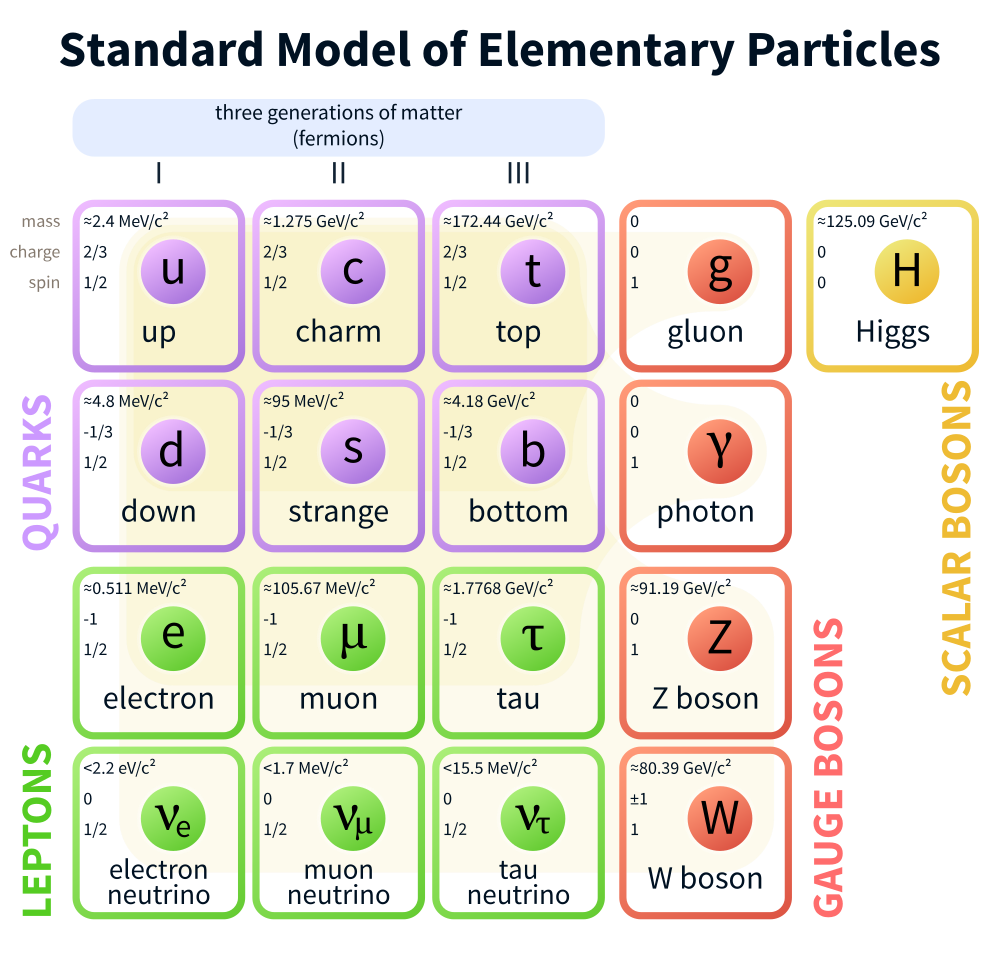
\includegraphics[width=\textwidth]{data/photo/theory/SM_particles.png}
\caption{The table for all fundamental particles in SM. \cite{SM_particles}}
\label{fig:SM_particles}
\end{figure}

\subsection{Matter particles}
There are six types of quarks: up quarks(u), down quarks(d), charm quarks(c), strange quarks(s), top quarks(t) and bottom quarks(b).
Quarks interact with strong interactions, while leptons do not.
There are three types of charged leptons: electrons, muons and taus.
There are three types of neutral leptons: electron neutrinos, muon neutrinos and tau neutrinos.
The first column is the first generation, which is the lightest and the most stable particles.
Hence, normal matter in our daily life is made from the particles in the first generation.
The second and third column are the second and third generation respectively, which are heavier and less stable particles.
These particles will finally decay into the particles in the first generation.
Due to the phenomenon of neutrino oscillation, neutrinos are massive, but their value are still unknown.

\subsection{Forces and carrier particles}
Photon is the force carrier of electromagnetic interactions.
Gluon is the force carrier of strong interactions.
Z and W bosons are the force carriers of weak interactions.
The effects of these fundamental forces stem from the exchange of the corresponding force carrier.
These forces also have different strengths and different interaction ranges.
The strong force is the strongest force, the electromagnetic force is in the middle, and the weak force is the weakest force.
The electromagnetic force has infinite range, while the strong and weak forces have very short ranges at the level of subatomic particles.

For example, a proton is composed of two up quarks and one down quark, and a neutron is composed of one up quark and two down quarks.
The forces between quarks inside the proton are mediated by gluons.

\subsection{Feynman diagram}
The fundamental interactions among these fundamental particles are described by the allowed Feynman vertices.
All these allowed Feynman vertices in the SM are shown in figures \ref{fig:vertices_SM} and \ref{fig:vertices_higgs}.

\begin{figure}
\centering
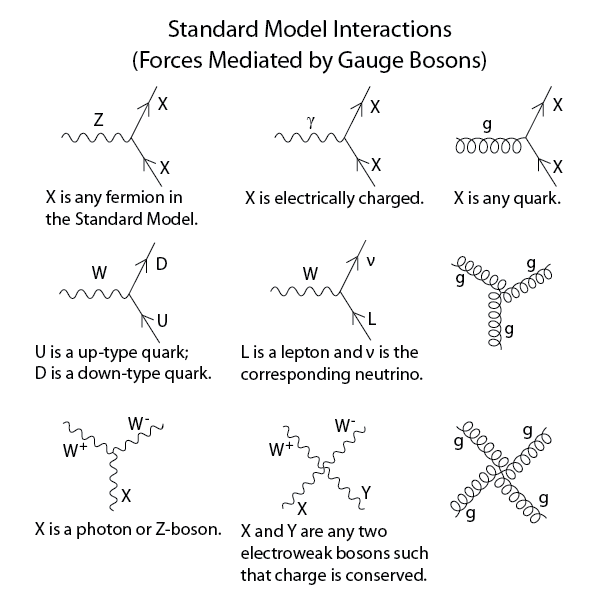
\includegraphics[width=\textwidth]{data/photo/theory/vertices_SM.png}
\caption{All allowed fundamental Feynman vertices in SM, except higgs-related vertices. \cite{vertices_SM}}
\label{fig:vertices_SM}
\end{figure}

\begin{figure}
\centering
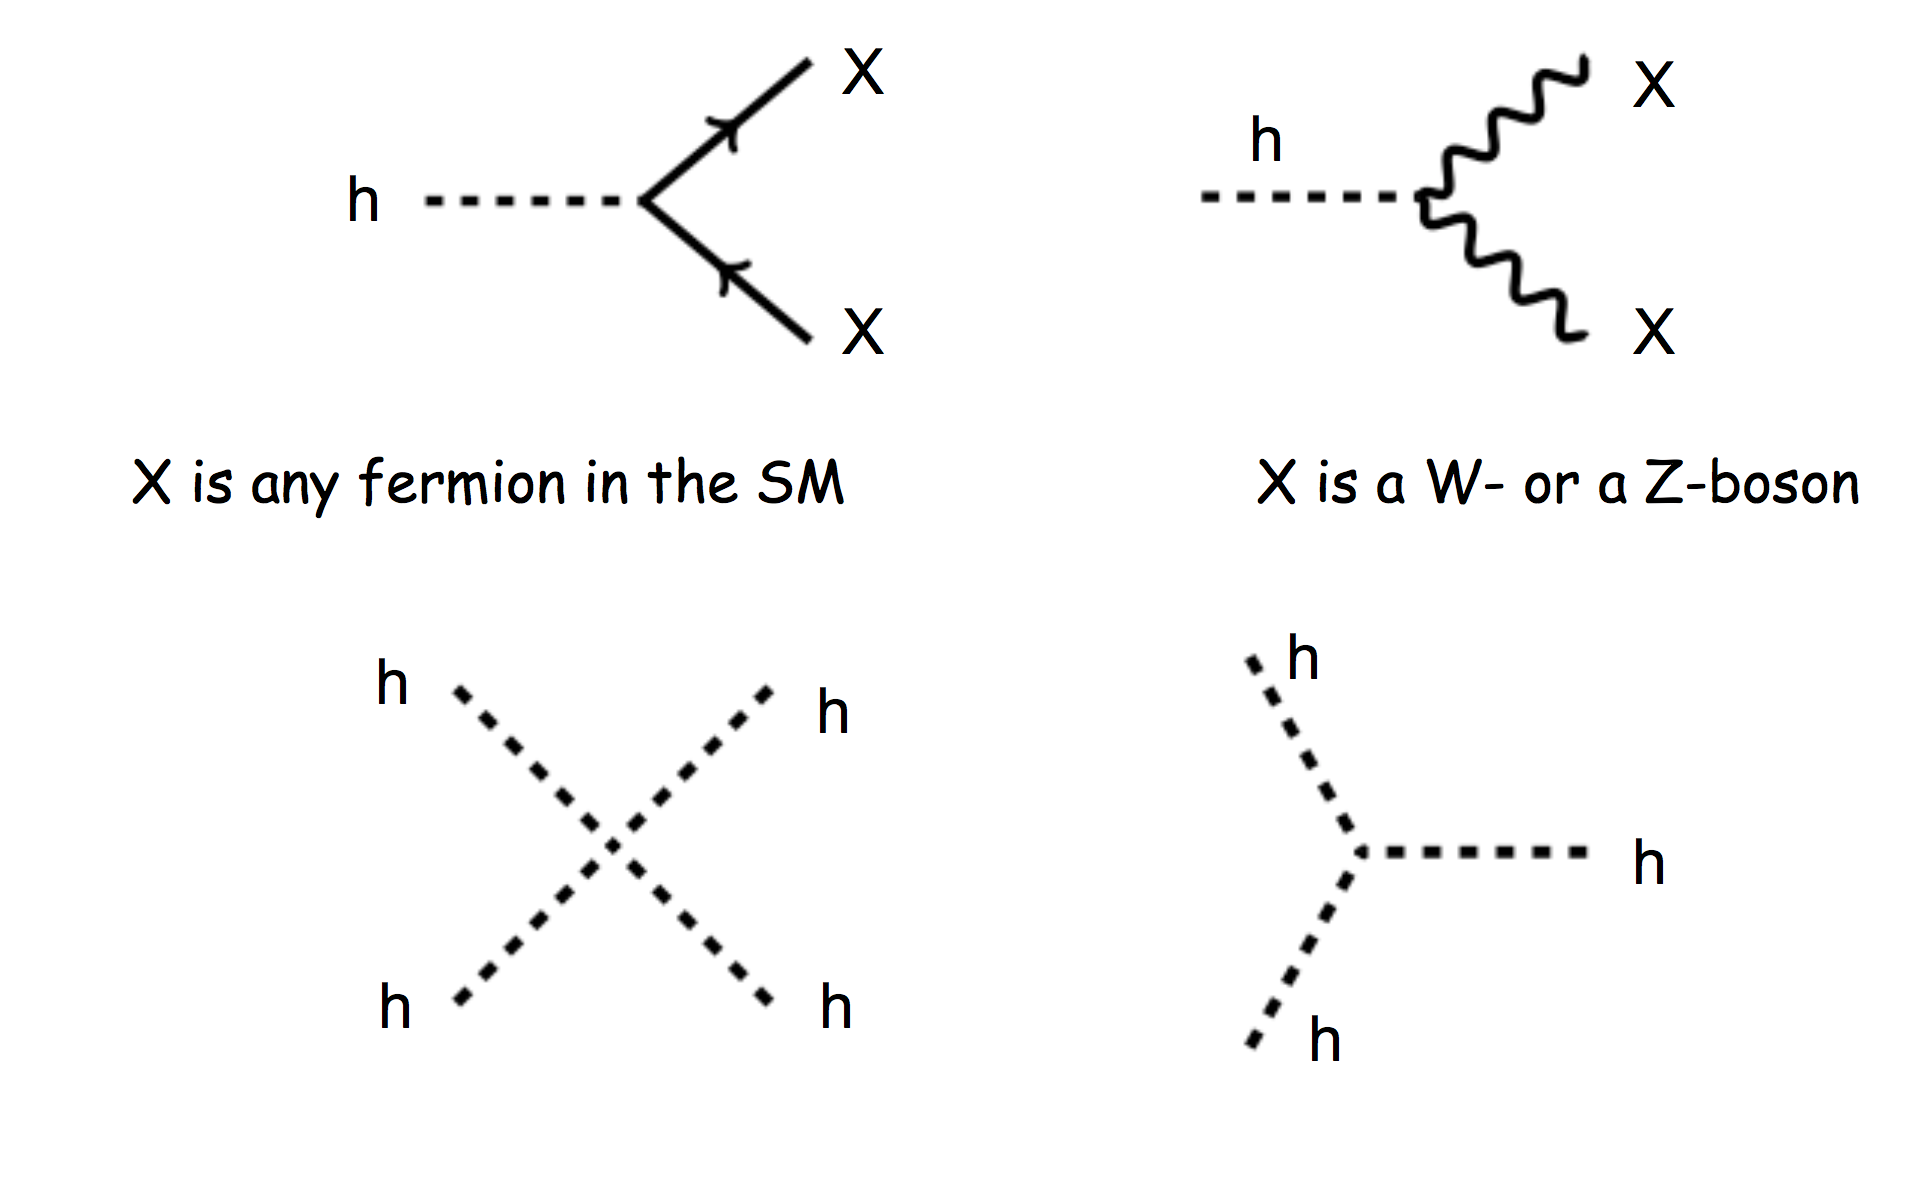
\includegraphics[width=\textwidth]{data/photo/theory/vertices_higgs.png}
\caption{All allowed fundamental higgs-related Feynman vertices in SM.}
\label{fig:vertices_higgs}
\end{figure}

\section{Limitation of Standard Model}
\label{sec:Limitation_Standard_Model}
Although the Standard Model can explain almost all experimental results, there are still some phenomena it cannot explain.

\subsection{Dark matter}
\label{sec:dark_matter}
Dark matter is some unknown matter that does not involve in electromagnetic interaction, but involves in gravitational interaction.
It was first discovered in the Milky Way, by studying the speed of the stars orbiting around the center of the Milky Way.
Because it does not involve in electromagnetic interaction, it cannot be seen by our telescopes.
However, the SM cannot explain what dark matter is.

\subsection{Hierarchy problem}
\label{subsec:hierarchy_problem}
The hierarchy problem is the question why the weak force is stronger than the gravitational force by $10^{24}$ times.
It is also asked why the mass of Higgs boson ($\sim 125$ GeV) is much lighter than the Planck mass ($\sim 10^{19}$ GeV).

The Lagrangian for the interaction term between the fermion Dirac field $f$ and the Higgs field $H$ (i.e. Yukawa interaction) is given by
\begin{equation}
\mathcal{L}_{\text{Yukawa}} = - \lambda_f \bar{f} H f
\end{equation}
where $\lambda_f$ is the Yukawa coupling constant.
The quantum correction to the square of the Higgs mass $\Delta m^2_H$ is then given by \cite{primer}
\begin{equation}
\Delta m^2_H = - \frac{|\lambda_f|^2}{8 \pi^2} \Big[ \Lambda^2 - 3 m_f^2 \ln \Big( \frac{\Lambda}{m_f} \Big) \Big] + \dots
\label{eq:higgs_correction}
\end{equation}
where $\Lambda$ is the energy scale up to which the quantum effects of gravity are not dominant, namely the Planck scale ($\sim 10^{19}$ GeV).
Because the first term is quadratic divergent in $\Lambda$, its correction to the Higgs mass is in the order of Planck scale.
Unless there are very delicate cancellation between the correction terms, the Higgs mass should be in the order of Planck scale.
But, we found that the experimental Higgs mass is in the order of 125 GeV, and this is called the hierarchy problem.

\subsection{Unification of forces}
In the 1860s, James Clerk Maxwell wrote down his famous equations Maxwell's equations, which unify two different phenomena: electricity and magnetism.
Due to this unification, we now understand that electricity and magnetism are two different manifestations of the same phenomenon, and we now call it electromagnetism.

Similar thing happened in the 1970s, physicists developed a theory that unified two fundamental forces: electromagnetic force and weak force.
At the energy scale above 246 GeV, these two forces will merge into a single force: electroweak force.
This unification predicted the existence of weak neutral current and a force carrier to carry this weak force.
This force carrier Z boson was later confirmed experimentally in CERN.

After that, an effect of strong force was found experimentally that the strong force becomes weaker when the energy scale is higher.
This may indicate that electroweak force and strong force will become a single force at higher energy scale.
There are some theories beyond the Standard Model that can unify these forces, such as supersymmetry.

\section{Supersymmetry}
Supersymmetry(SUSY) is a theoretical extension of the Standard Model, and can answer some questions which the Standard Model cannot answer, mentioned in section \ref{sec:Limitation_Standard_Model}.
One of the problems SUSY can solve is the hierarchy problem of Higgs mass mentioned in section \ref{subsec:hierarchy_problem}.
We first notice that the negative sign of the quadratic divergent term in the equation \ref{eq:higgs_correction} is due to the correction from the fermions.
If there is a symmetry between the fermions and bosons, and the quadratic terms due to the bosons cancel with the quadratic terms due to the fermions, the hierarchy problem can be solved.
This new symmetry is called the supersymmetry (SUSY).

\subsection{Minimal Supersymmetric Standard Model}
Minimal Supersymmetric Standard Model(MSSM) is the simplest realization of the supersymmetric theory that contains the minimum number of new particles and new interactions.
It predicts that each particle in the Standard Model has its own partner particle, called the superpartner, as shown in figure \ref{fig:SUSY_particles}.
This is the new symmetry between the fermions and bosons.
The name scheme for the superpartner of a fermion is to add a prefix ``s'', in front of the name of the original Standard Model particle: squarks and sleptons, etc.
For example, the superpartner of an electron is called selectron.
For the superpartner of a Standard Model boson, the suffix ``ino'' is added: gluino and Higgsino, etc.
As for the symbol for the superpartner, a tilde is added above the original symbol.
For example, the symbol for selectron is $\tilde{e}$.
Also, the spin of the superpartner differs from the Standard Model particle by 1/2.
For fermions, the spin of their superpartner is 0, while for bosons, the spin of their superpartner is 1/2.
The superpartners interact with the same forces as the Standard Model particles, but they have different masses.

\begin{figure}
\centering
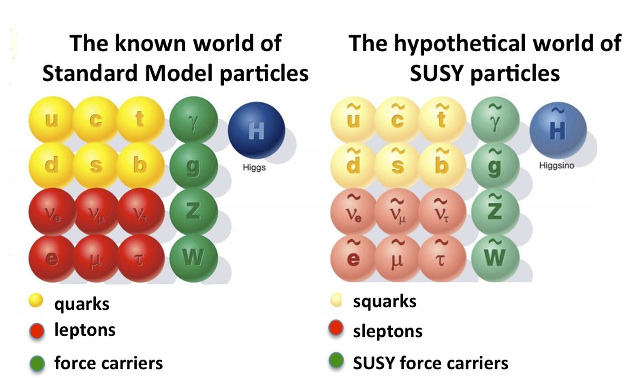
\includegraphics[width=\textwidth]{data/photo/theory/SM-SUSY-diagram.jpg}
\caption{The particles in Standard Model and their corresponding superpartners and their names}
\label{fig:SUSY_particles}
\end{figure}

The quantum correction terms from the superpartners cancel the quadratic divergent terms in the Higgs mass.
The idea is to postulate two scalar fields $\tilde{f}$ for each fermion, with the coupling constant to the Higgs $\lambda_{\tilde{f}}$.
\begin{equation}
\mathcal{L} = - \lambda_{\tilde{f}} |H|^2 |\tilde{f}|^2
\end{equation}
The quantum correction to the square of the Higgs mass $\Delta m^2_H$ for the scalar field is given by \cite{primer}
\begin{equation}
\Delta m^2_H = \frac{ \lambda_{\tilde{f}} }{16 \pi^2} \Big[ \Lambda^2 - 2 m_{\tilde{f}}^2 \ln \Big( \frac{\Lambda}{m_{\tilde{f}}} \Big) \Big] + \dots
\label{eq:higgs_correction2}
\end{equation}
The quadratic terms in \ref{eq:higgs_correction} and \ref{eq:higgs_correction2} exactly cancel with each other, if $\lambda_{\tilde{f}} = |\lambda_f|^2$.
The logarithmic terms are left in the correction terms for the Higgs mass.
Therefore, the hierarchy problem is solved.

In the MSSM, two neutral Higgs bosons ($H^0_u$ and $H^0_d$) and two charged Higgs bosons ($H^+_u$ and $H^-_d$) are introduced.
Therefore, there are 4 neutral bosons: $\gamma$, $Z$, $H^0_u$, $H^0_d$ and 4 charged bosons: $W^+$, $W^-$, $H^+_u$ ,$H^-_d$.
The superpartners of the four neutral bosons together form four mass eigenstates called neutralinos: $\tilde{\chi}_1^0$, $\tilde{\chi}_2^0$, $\tilde{\chi}_3^0$ and $\tilde{\chi}_4^0$.
The superpartners of the four charged bosons together form two mass eigenstates with electric charge $\pm 1$, called charginos: $\tilde{\chi}_1^\pm$ and $\tilde{\chi}_2^\pm$.
The subscripts of the symbol of the neutralinos and charginos are labeled by the ascending order in mass.
Table \ref{tab:SUSY_particle} summarizes the Standard Model particles and their superpartners.

\begin{table}[htbp]
\tiny
\centering
\begin{tabular}{|c|cccc|cccc|}
\hline
\hline
Type & SM particle & Symbol & Spin & R-parity & Superpartner & Symbol & Spin & R-parity \\
\hline
\hline
Fermions & Quark  & $q$ & $\frac{1}{2}$ & +1 & Squark  & $\tilde{q}$ & 0 & -1 \\
         & Lepton & $l$ & $\frac{1}{2}$ & +1 & Slepton & $\tilde{l}$ & 0 & -1 \\
\hline
Gluon & Gluon  & $g$ & $1$ & +1 & Gluino & $\tilde{g}$ & $\frac{1}{2}$ & -1  \\
\hline
Neutral EW Bosons & Photon         & $\gamma$ & $1$ & +1
                  &  &  &  &  \\
                  & Z Boson        & $Z$      & $1$ & +1
                  & Neutralinos & $\tilde{\chi}_1^0$, $\tilde{\chi}_2^0$, $\tilde{\chi}_3^0$, $\tilde{\chi}_4^0$ & $\frac{1}{2}$ & -1 \\
                  & Neutral Higgs  & $H^0_u$, $H^0_d$  & $0$ & +1
                  &  &  &  &  \\
\hline
Charged EW Bosons & W Boson        & $W^+$, $W^-$  & $1$ & +1
                  & Charginos & $\tilde{\chi}_1^\pm$, $\tilde{\chi}_2^\pm$ & $\frac{1}{2}$ & -1 \\
                  & Charged Higgs  & $H^+_u$, $H^-_d$  & $0$ & +1
                  &  &  &  &  \\
\hline
\hline
\end{tabular}
\caption{The spin and R-parity for the Standard Model particles and their superpartners.}
\label{tab:SUSY_particle}
\end{table}

The baryon number $B$ is defined by $\frac{1}{3} (n_q - n_{\bar{q}})$, where $n_q$ is the number of quarks and $n_{\bar{q}}$ is the number of anti-quarks.
The lepton number $L$ is defined by $n_l - n_{\bar{l}}$, where $n_l$ is the number of leptons and $n_{\bar{l}}$ is the number of anti-leptons.
In the Standard Model and the experimental data, $B-L$ is conserved, but in MSSM, it is no longer conserved.
To keep this conservation and prevent the proton decay, the R-parity $P_R$ is introduced.
\begin{equation}
P_R = (-1)^{3(B-L)-2s}
\end{equation}
where s is the spin.
By this definition, all Standard Model particles have R-parity $+1$, and all supersymmetric particles have R-parity $-1$.
If the R-parity is conserved, the lightest supersymmetric particle (LSP) does not decay.
If the LSP is electrically neutral and interacts with matter only by the weak interaction and gravity, for example the lightest neutralinos $\tilde{\chi}_1^0$ or a sneutrino $\tilde{\nu}$, it can be a candidate for dark matter mentioned in section \ref{sec:dark_matter}.
In this analysis, the R-parity is assumed to be conserved, and the lightest neutralino $\tilde{\chi}_1^0$ is assumed to be the LSP.
Due to the conservation of R-parity, the supersymmetric particles can only be pair-produced, and eventually decay into Standard Model particles and the lightest neutralino $\tilde{\chi}_1^0$, i.e. the LSP.

\section{Signal scenario}
\label{sec:Wh_signal}
In the recent searches for the squarks and gluinos, the masses of gluinos and the first and second generation squarks are suggested to be larger than 1 TeV, while the upper mass limits of the third generation squarks are below 1 TeV \cite{gluinos}.
In this case, the direct pair production of electroweak gauginos (i.e. neutralinos and charginos) can be the dominant SUSY production process at the LHC, if the masses of the gluinos and squarks are significantly heavier than the low mass electroweak gauginos.
Based on the results in the Run-I analysis \cite{run1} at the center-of-mass energy $\sqrt{s} = 8$ TeV shown in figure \ref{fig:result_run1}, the electroweak pair production is a promising search at a higher center-of-mass energy $\sqrt{s} = 13$ TeV with Run-II using 2015 and 2016 data.

\begin{figure}
\centering
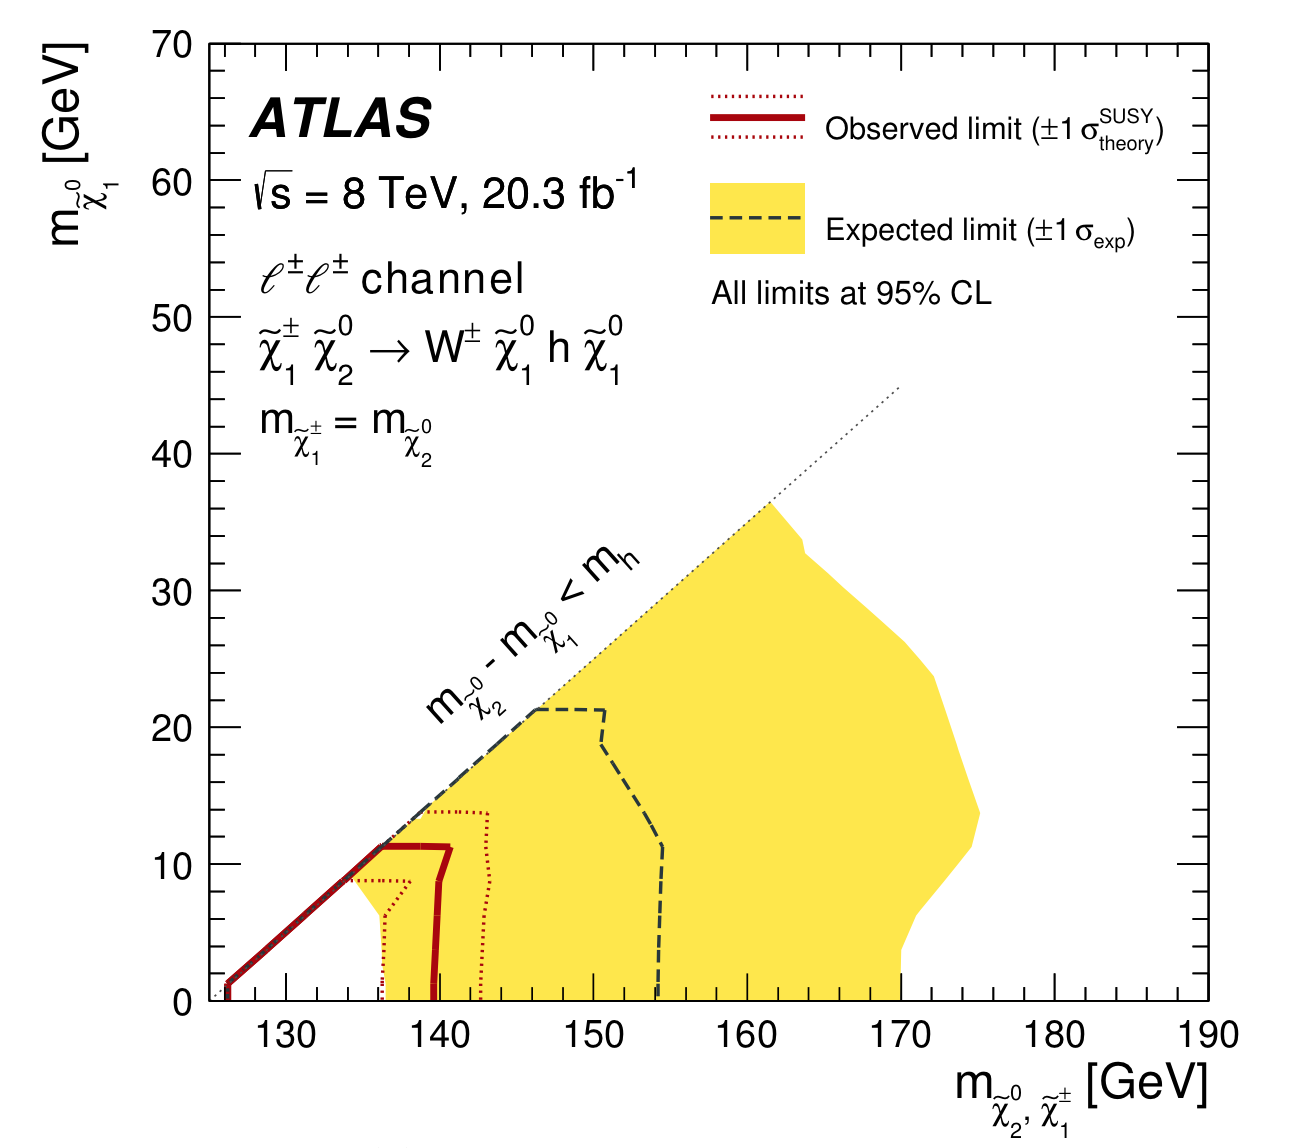
\includegraphics[width=0.5\textwidth]{data/photo/theory/run1.png}
\caption{The exclusion contours for the masses $m_{\tilde{\chi}_1^\pm , \tilde{\chi}_2^0}$ and $m_{\tilde{\chi}_1^0}$ in the Run-I analysis \cite{run1}.}
\label{fig:result_run1}
\end{figure}

The supersymmetric process searched in this thesis is the pair production of the lightest chargino $\tilde{\chi}_1^\pm$ and the second lightest neutralino $\tilde{\chi}_2^0$.
The masses of them are assumed to be the same, $m_{\tilde{\chi}_1^\pm} = m_{\tilde{\chi}_2^0}$, and denoted by $m_{\tilde{\chi}_1^\pm , \tilde{\chi}_2^0}$ in the following chapters.
With the assumption that all sleptons are heavier than $\tilde{\chi}_1^\pm$ and $\tilde{\chi}_2^0$,
$\tilde{\chi}_1^\pm$ decays to W boson and $\tilde{\chi}_1^0$ (i.e. $\tilde{\chi}_1^\pm \rightarrow W^{\pm} + \tilde{\chi}_1^0$)
and $\tilde{\chi}_2^0$ decays to the lightest MSSM Higgs boson $h$ and $\tilde{\chi}_1^0$ (i.e. $\tilde{\chi}_2^0 \rightarrow h + \tilde{\chi}_1^0$),
or Z boson and $\tilde{\chi}_1^0$ (i.e. $\tilde{\chi}_2^0 \rightarrow Z + \tilde{\chi}_1^0$).
In this thesis, we assume $\tilde{\chi}_1^\pm \rightarrow W^{\pm} + \tilde{\chi}_1^0$ and $\tilde{\chi}_2^0 \rightarrow h + \tilde{\chi}_1^0$ with 100\% branching ratio.
The mass of the lightest MSSM Higgs boson $h$ is set to be 125 GeV.

The W boson from $\tilde{\chi}_1^\pm$ decays into one lepton (electron or muon) and one neutrino (i.e. $W{^\pm} \rightarrow \ell^{\pm} + \nu$).
The Higgs boson from $\tilde{\chi}_2^0$ eventually decays into one lepton (electron or muon), quarks (i.e. jets) and neutrino(s) by various decay modes.
For example, $h \rightarrow W^{+} W^{-} $ and $h \rightarrow \tau^{+} \tau^{-} $ are the dominant decay modes, with one of the $W / \tau$ decays leptonically (e.g. $W{^\pm} \rightarrow \ell^{\pm} + \nu$) and another decays hadronically (e.g. $W \rightarrow q + q$).
Figure \ref{fig:signal_feynman} is the Feynman diagram for the signal process searched in this thesis.

\begin{figure}
\centering
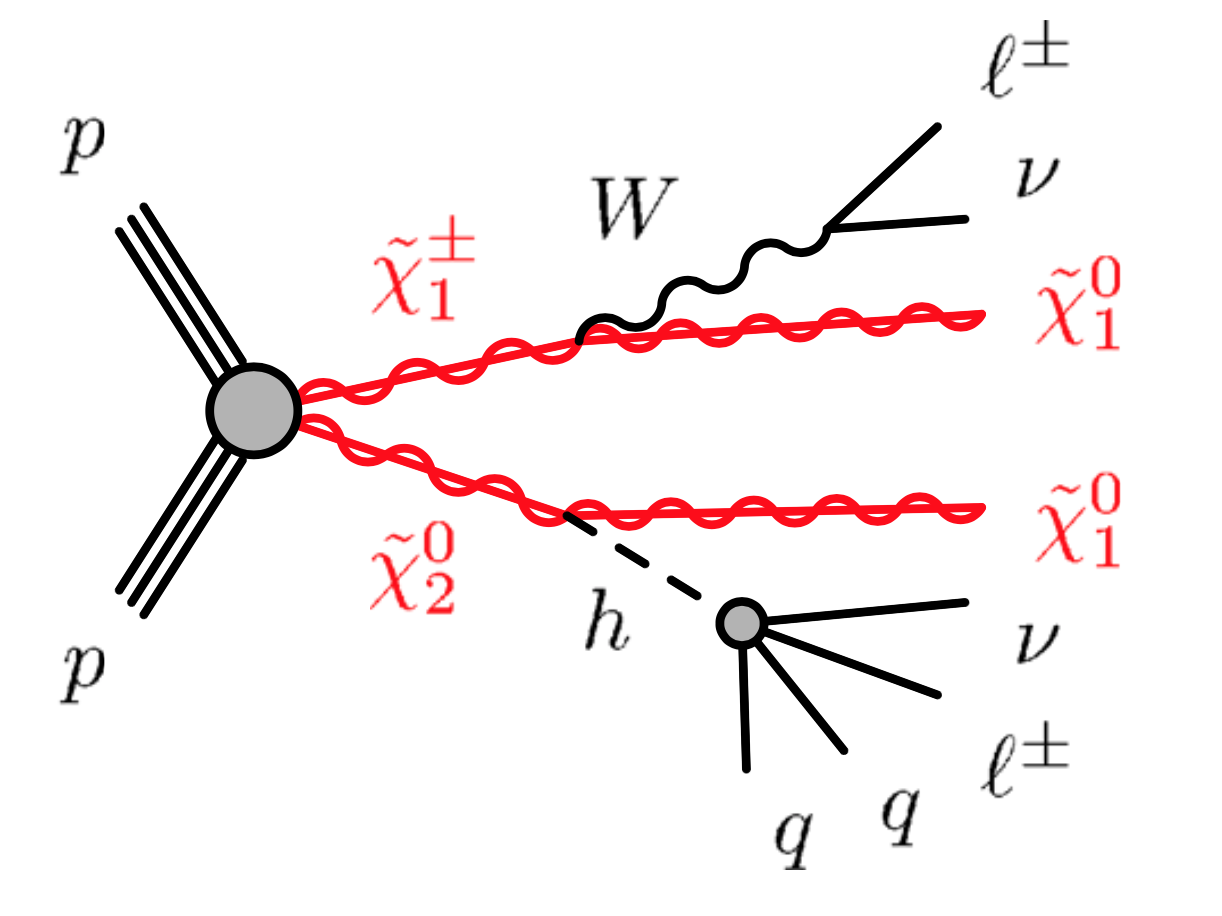
\includegraphics[width=0.5\textwidth]{data/photo/theory/signal_feynman.png}
\caption{The Feynman diagram for the Wh same-sign signal scenario in this thesis. The final states in this process include two same-sign leptons (electron or muon), quarks (i.e. jets) and missing transverse momentum contributed by the lightest neutralinos $\tilde{\chi}_1^0$ and neutrinos $\nu$.}
\label{fig:signal_feynman}
\end{figure}

The two leptons in the final states are either electrons or muons, and the term ``lepton'' (with symbol $\ell$) in the following chapters refers to electron or muon, but not tau lepton or neutrino.
We search for the final state with exactly two leptons with the same electric charge, which rarely exists in the Standard Model.
In the case that mass splitting is close to the mass of Higgs boson, which is called the compressed region, one of the lepton could be very soft that it fails the requirement of the signal lepton, due to the low momentum of the Higgs boson.
However, if the Higgs boson eventually decays into two leptons, for example $h \rightarrow ZZ$ with one of the Z boson decaying leptonically (e.g. $Z \rightarrow \ell^{+} + \ell^{-}$) and another decaying hadronically (e.g. $Z \rightarrow q + q$), the total number of leptons in the final state is three.
If one of the three leptons is soft and another two leptons have the same electric charge, this scenario will have the same final state as our signal.
This means that in the compressed region, our 2-leptons search channel would be more sensitive than the 3-leptons channel.

Because the two neutralinos $\tilde{\chi}_1^0$ and neutrinos $\nu$ in the final state cannot be detected, a large missing transverse momentum (i.e. unbalanced momentum in the detector) is expected.

This analysis is a collaborative work with other people and the results are mainly based on the paper \cite{Wh} and the internal note \cite{WhSS}.

%************************************************
\chapter{Experimental Setup}
\label{ch:detector}
%************************************************

\section{Introduction}
\label{sec:detector_introduction}

Our experimental data was collected from the ATLAS particle detector in the Large Hadron Collider (LHC).
The following section will introduce LHC and the ATLAS particle detector.

\section{The Large Hadron Collider}
\label{sec:detector_LHC}

The Large Hadron Collider (LHC) was built in the border between France and Switzerland by the European Organization for Nuclear Research (CERN).
It is a circular particle collider under the ground with circumference 27 km.
Two beams of protons will be accelerated in opposite directions, and then these two beams will collide with each other at the collision point.
The energy of each beam is 6.5 TeV, and hence the center-of-mass energy of the two beams $\sqrt{s}$ is 13 TeV, which is the energy used in this experiment.
This energy is equivalent to the speed that the beam will circulate the ring 11,245 times per second.
Figure \ref{fig:detector_LHC_accelerator_complex} shows the schematic diagram of the CERN accelerator complex, which contains a series of accelerators, from low energy to high energy.
The dark blue big circle in figure \ref{fig:detector_LHC_accelerator_complex} represents the LHC, on which there are 4 particle detectors at 4 different yellow points: ATLAS, CMS, LHCb and ALICE.

\begin{figure}
\centering
\includegraphics[width=\textwidth]{data/photo/accelerator_complex.png}
\caption{The schematic diagram of the CERN accelerator complex, which shows a series of accelerators and facilities. \cite{complex}}
\label{fig:detector_LHC_accelerator_complex}
\end{figure}

Before the beam is injected into LHC, the protons need to be accelerated by a series of accelerators.
The journey of the protons starts from a tank of hydrogen gas.
The proton and the electron are separated by a electric field.
The protons are then accelerated to 50 MeV by Linac2, which is a linear accelerator.
The beam is then injected to the second accelerator called the Proton Synchrotron Booster (PSB), which accelerates the beam to 1.4 GeV.
The beam is then injected to the third accelerator called the Proton Synchrotron (PS), which pushes the beam to 25 GeV.
The beam is then injected to the fourth accelerator called the Super Proton Synchrotron (SPS), which further pushes the beam to 450 GeV.
Finally, the beam is injected to the two beam pipes of the LHC.
One of the beam moves in clockwise direction, while another beam moves in anti-clockwise direction.
Two beams will be collided at the collision point inside the ATLAS detector.
\cite{accelerator}

The circular path of the proton beam is maintained by many superconducting electromagnets along the LHC tunnel.
There are 1232 main magnetic dipoles, and each of them generates a large magnetic field of 8.3 T.
In order to generate such a high magnetic field, the coils need to have very high currect of 11,080 A, and hence supercoducting coil need to be used, to reduce the heat loss due to the electrical resistance.
The material of supercoducting coil is niobium-titanium (NbTi).
To reach the condition for supercoductivity, the electromagnets operate at a very low temperature of 1.9 K.
There are also 392 magnetic quadrupole to make the beam narrower, and the chance of proton-proton collision will be higher.
\cite{supermagnet,cryogenics}

The protons in the beam are grouped into different bunches, and there are about $10^{11}$ protons in each bunch.
The time-spacing between two adjacent bunches is 25ns (or 50 ns in the old configuration).
This means that in each 25 ns, two bunches are collided at the collision point.
For each bunch collision, there are about 10 to 50 proton-proton interaction.

The interacting rate for a physics proccess $\frac{dN}{dt}$ is the product of the cross section of that physics proccess $\sigma$ and the instantaneous luminosity $\mathcal{L}$.
\begin{equation}
\frac{dN}{dt} = \sigma \mathcal{L}
\end{equation}
The instantaneous luminosity $\mathcal{L}$ is a measure of the interacting rate of two protons at the collision point, which is related to the density of the protons and the speed of the protons.
The instantaneous luminosity in this experiment is about $10^{34}$ cm$^{-2}$ s$^{-1}$ (or 10 nb$^{-1}$ s$^{-1}$).

\section{ATLAS detector}
\label{sec:detector_ATLAS}

A Toroidal LHC ApparatuS (ATLAS) is the particle detector used in this experiment \cite{ATLAS_doc}.
Figure \ref{fig:detector_ATLAS} shows the main components of the ATLAS detector.
\begin{figure}
\centering
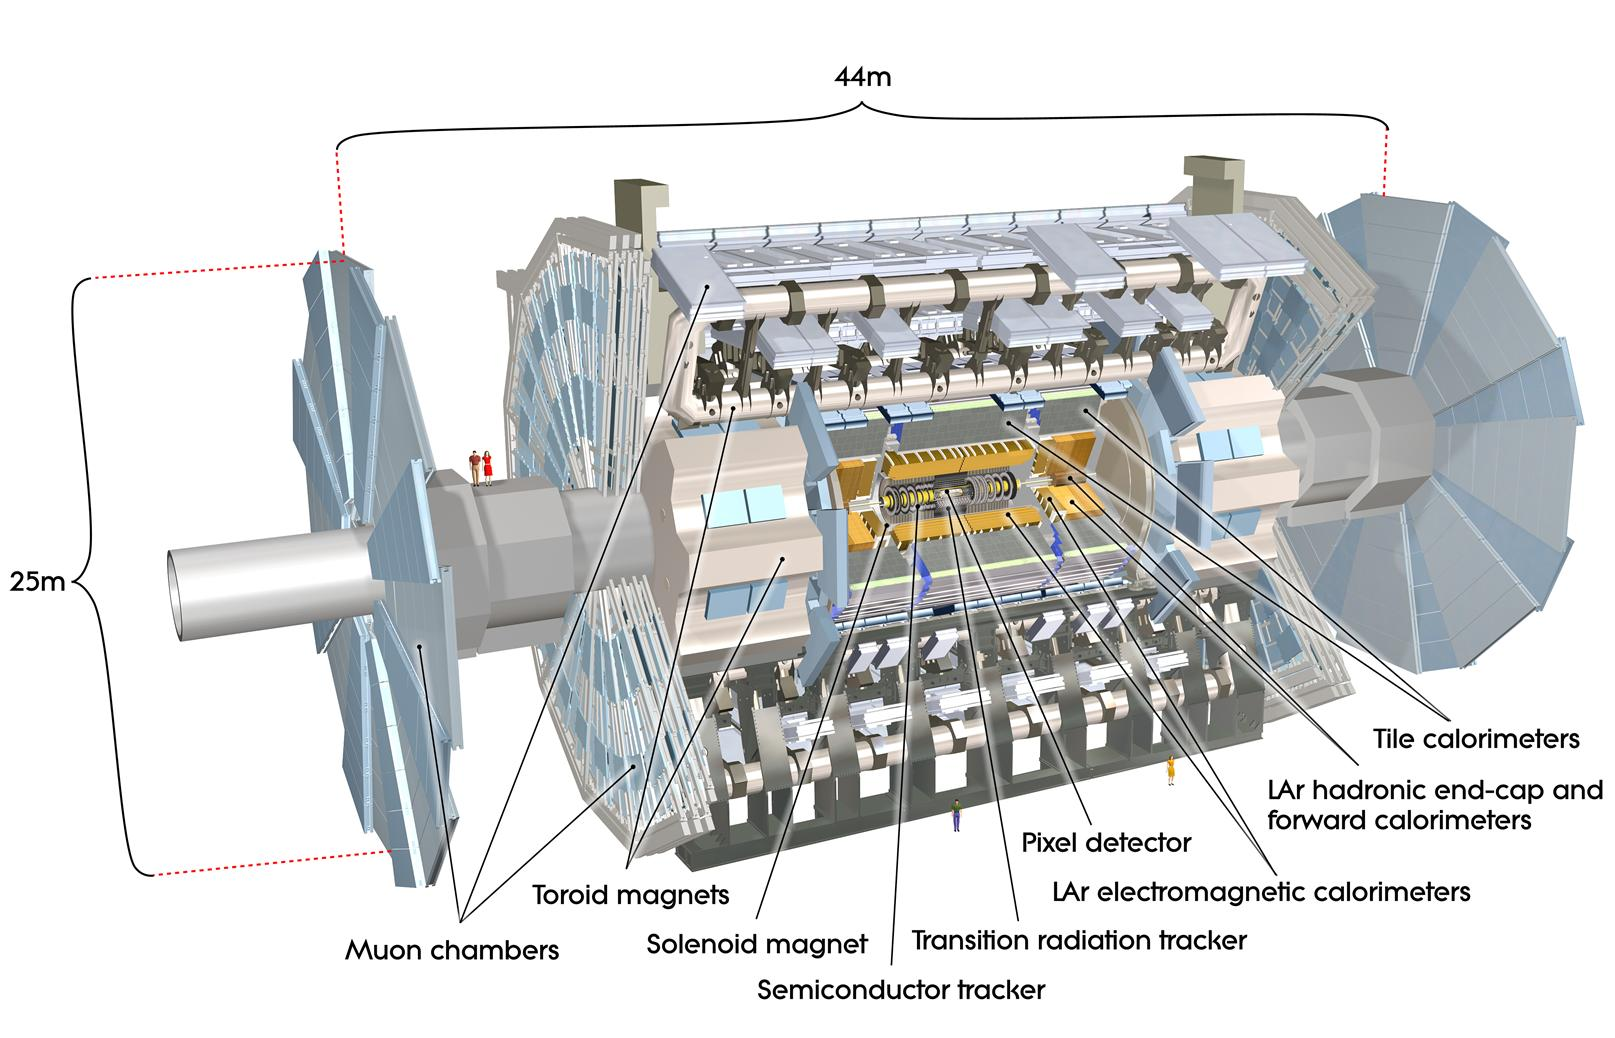
\includegraphics[width=\textwidth]{data/photo/ATLAS.jpg}
\caption{The cut-away view of the ATLAS detector. It is 25m high and 44m long. \cite{ATLAS_photo}}
\label{fig:detector_ATLAS}
\end{figure}
The ATLAS detector is a general purpose particle detector, which is consisted of 3 main components: the inner detector, the calorimeter and the muon spectrometer.
Figure \ref{fig:ATLAS_particles} shows how the ATLAS distinguishes different types of particle. The inner detector can detect the paths of the charged particles.
Photons and electrons will deposit most of their energy in the electromagnetic calorimeter, and finally stop by it.
Hadrons(including protons and neutrons) and mesons will similarly stop by the hadronic calorimeter.
Only muons and the neutrinos can reach the outermost muon spectrometer, but only muons can be detected by the muon spectrometer.
Nearly all neutrinos will escape the whole ATLAS detector, which leads to some missing energy.
In this design, different particles can be identified due to their signature in different parts of ATLAS.
\begin{figure}
\centering
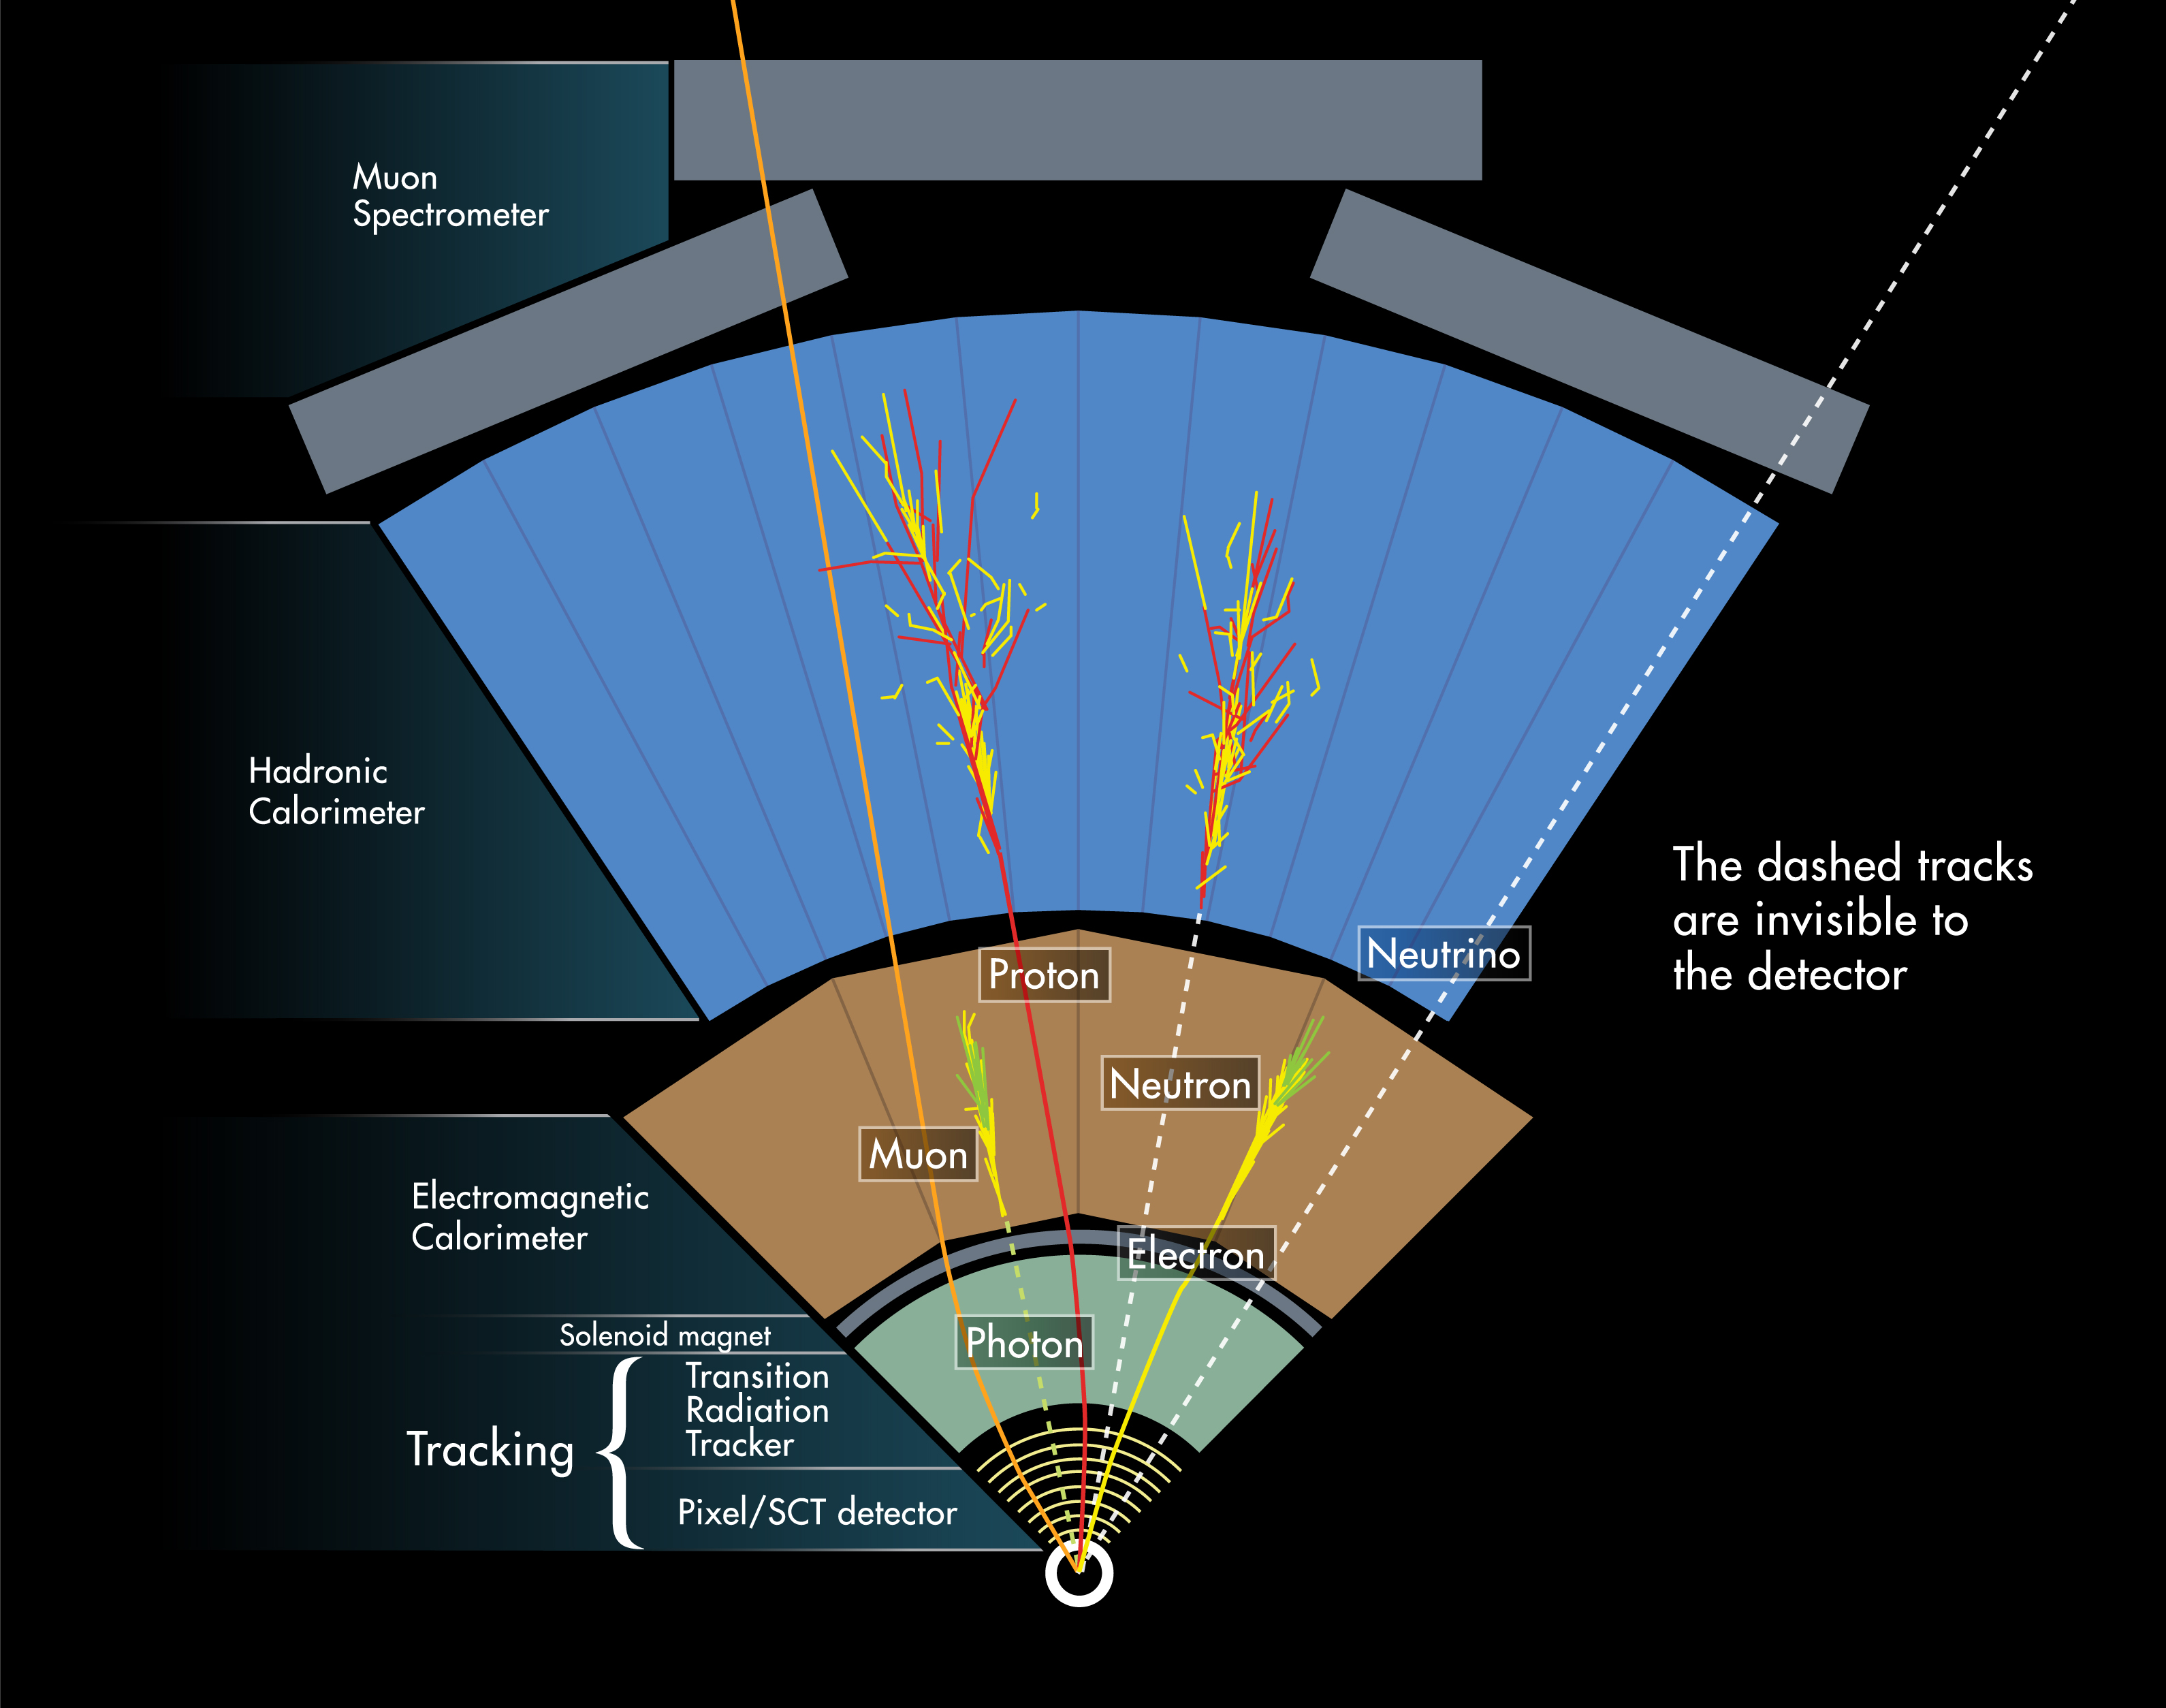
\includegraphics[width=\textwidth]{data/photo/ATLAS_particles.jpg}
\caption{The cross section of the ATLAS detector. This shows different components of the ALTAS and how ATLAS detect different types of particles \cite{ATLAS_particles}}
\label{fig:ATLAS_particles}
\end{figure}

\subsection{coordinate system}
The nominal collision point is defined as the origin of the coordinate system.
The z-axis is along the beam dirention.
The positive x-asix is pointing to the centre of the LHC ring.
The positive y-asix is in the upward direction.
The azimuthal angle $\phi$ and the polar angle $\theta$ are defined as usual in the spherical coordinate system.
The pseudorapidity $\eta$ is defined as:
\begin{equation}
\eta = - \ln \Big( \tan \frac{\theta}{2} \Big)
\end{equation}
The distance $\Delta R$ in the pseudorapidity-azimuthal angle space is defined as:
\begin{equation}
\Delta R = \sqrt{(\Delta \phi) ^2 + (\Delta \eta) ^2}
\end{equation}
The ATLAS detector has a reflection symmetry about the x-y plane.

\subsection{magnetic system}
There is a thin superconducting solenoid magnet around the inner detector, which generates a 2 T magnetic field inside the inner detector.
There are also 3 large superconducting toroids around the calorimeter: one for barrel and two for end-caps.
All these magnets are shown in figure \ref{fig:detector_ATLAS}.

\subsection{The inner detector}
The inner detector is a particle tracker.
It mainly detects the tracks of charged particles and has good performance for measuring the momentum of the charged particles and locating the position of the vertices.
Figure \ref{fig:detector_inner_whole} shows the whole structure of the inner detector.
The inner detector consists of 3 sub-detectors from inner to outer: the pixel detector, the silicon microstrip tracker (SCT) and the transition radiation tracker (TRT).
Each part further divides into two parts: the barrel region with smaller $|\eta|$ and the end-cap region with larger $|\eta|$.
Figure \ref{fig:detector_inner_detail} shows the distances R from the beam for the 3 sub-detectors, and figure \ref{fig:detector_inner_size} shows the shapes and the orientations of each sensor and the $\eta$ coverage, in both the barrel and the end-cap regions.
The $\eta$ coverage for the inner detector is $|\eta| < 2.5$.
The shapes and the orientations of the sensors are different in the barrel and the end-cap regions.
In the barrel region, the shape and the orientation of the sensors is concentric cylinder shells around the beam axis, while in the end-cap region, they are disks perpendicular to the beam axis.
\begin{figure}
\centering
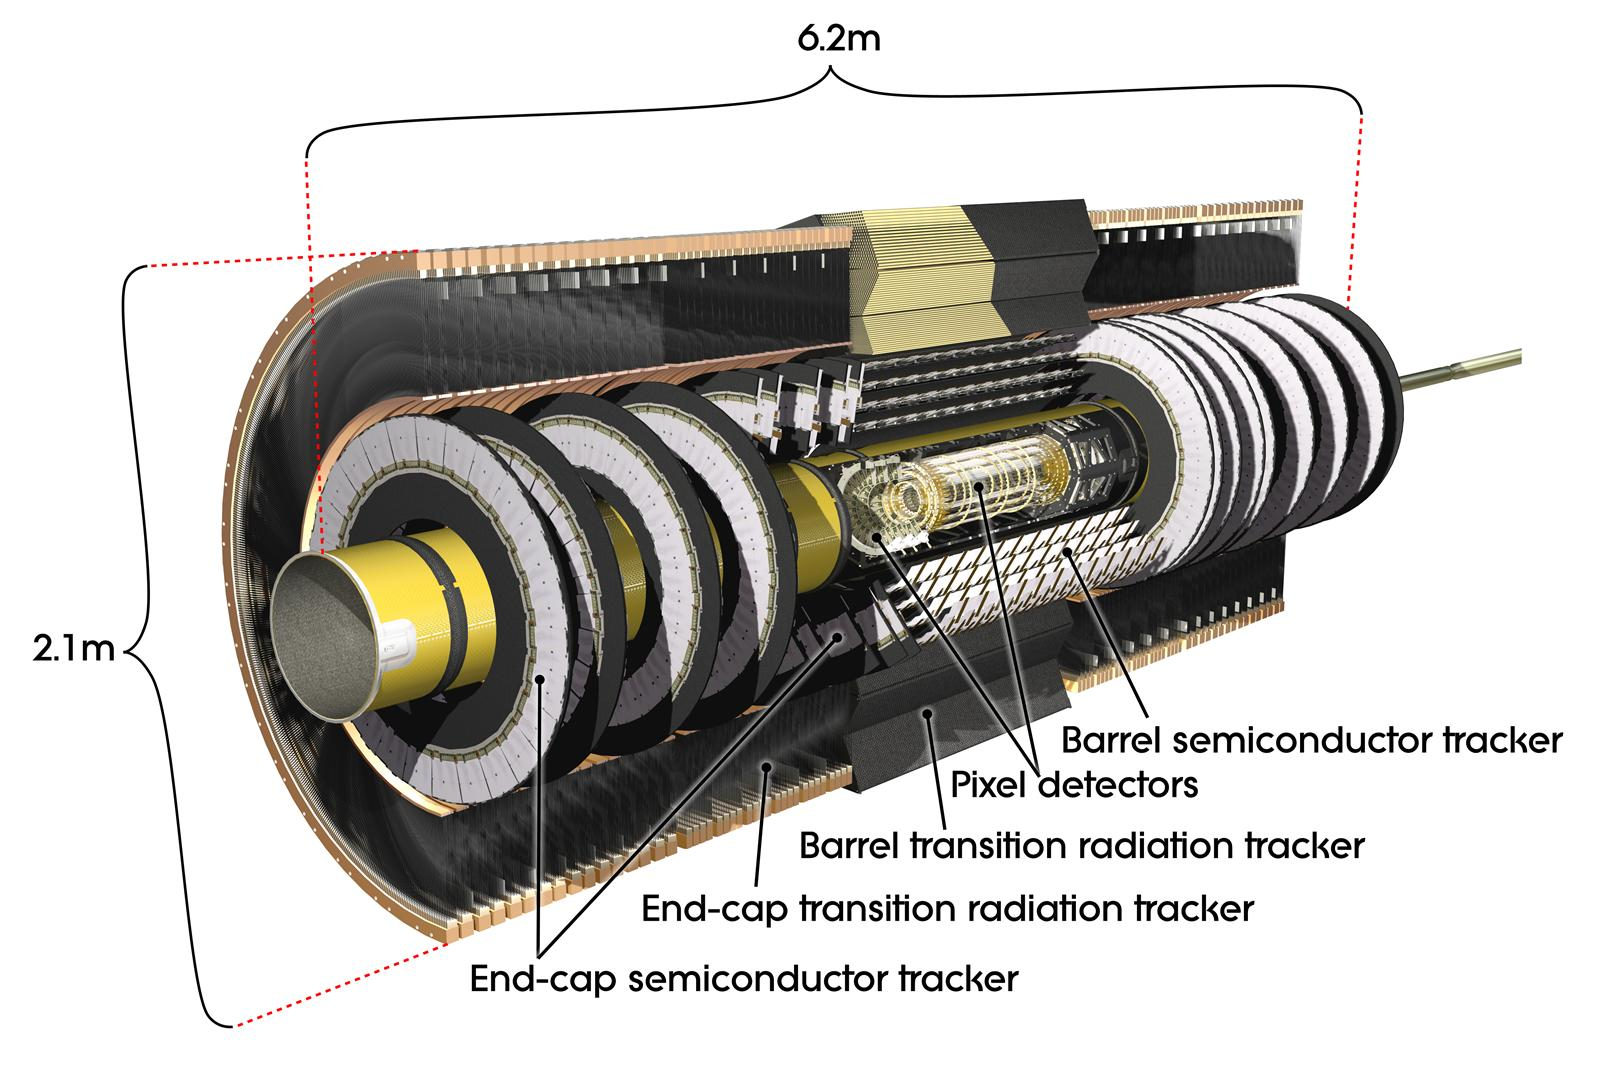
\includegraphics[width=\textwidth]{data/photo/inner_whole.jpg}
\caption{The whole structure of the ATLAS inner detector. \cite{inner_photo}}
\label{fig:detector_inner_whole}
\end{figure}
\begin{figure}
\centering
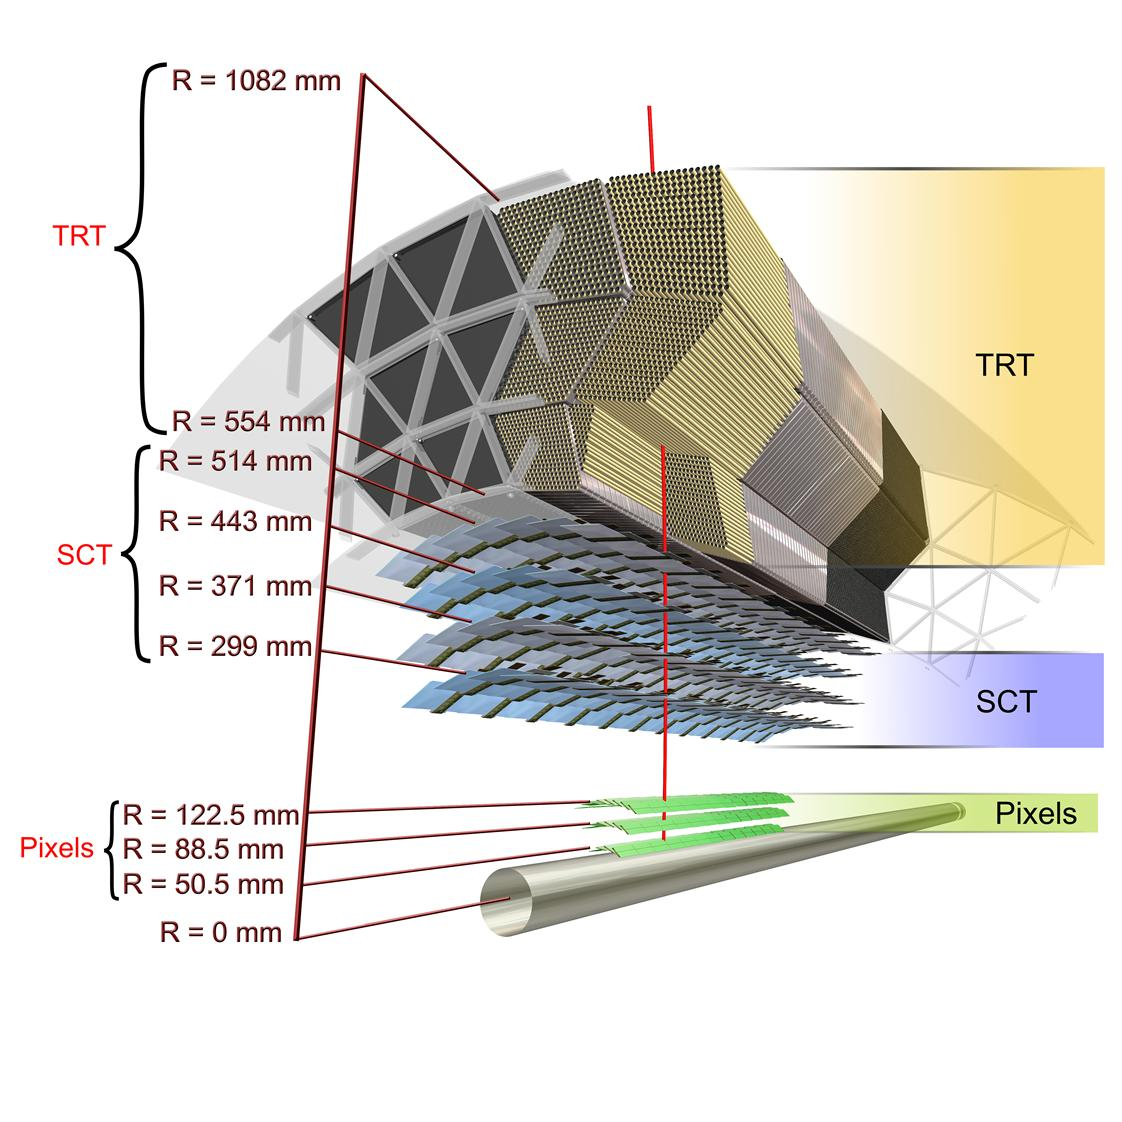
\includegraphics[width=\textwidth]{data/photo/inner_detail.jpg}
\caption{The distances R from the beam for the 3 components: pixel, SCT and TRT. \cite{inner_photo}}
\label{fig:detector_inner_detail}
\end{figure}
\begin{figure}
\centering
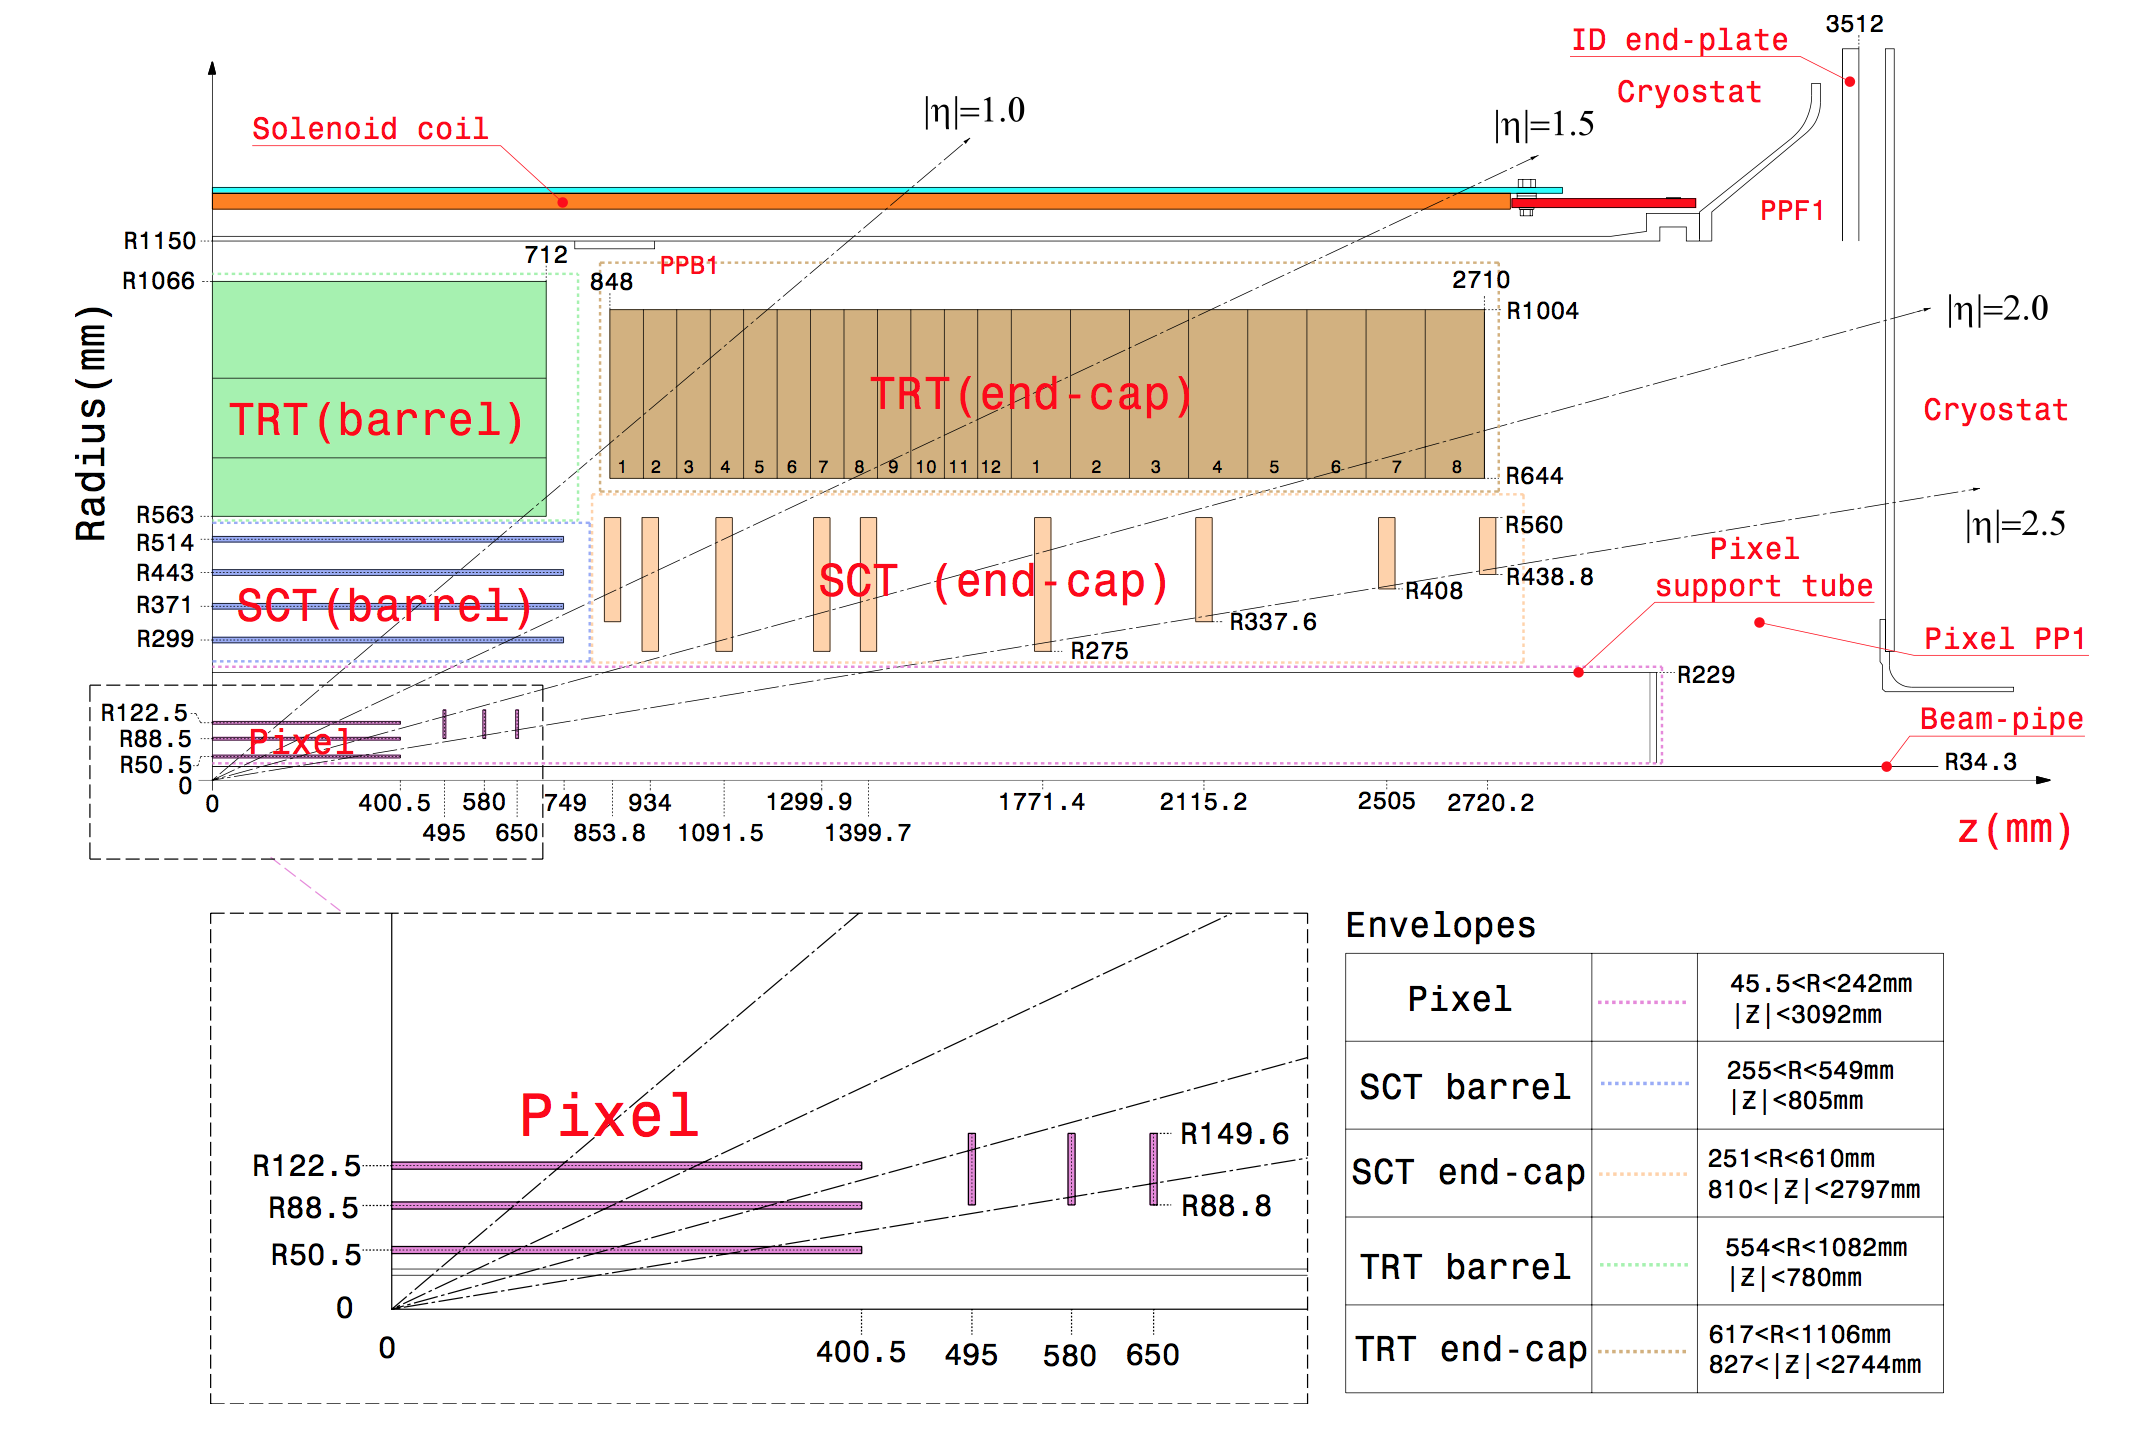
\includegraphics[width=\textwidth]{data/photo/inner_size.png}
\caption{The shapes, the orientations and the $\eta$ coverage for each sensor. \cite{ATLAS_doc}}
\label{fig:detector_inner_size}
\end{figure}

The precision tracking detectors (pixels and SCT) has high resolution in space by using discrete space-points to detect the track of a charged particle, with the cutting-edge technology, in order to achieve the good performance of the inner detector.
When the particle moves inside the inner detector, there are, in average, 36 hits per one track.
By recording the positions of these hits, the path of the particle can be reconstructed.
The whole inner detector is immersed in a 2 T magnetic field generated by the solenoid magnet, and hence the path of any charged particles will be bent.
By measuring the curvature of the path, the charge and momentum of the particle can be measured.
The equation for the circular path is
\begin{equation}
\frac{d\mathbf{p}}{dt} = q(\mathbf{v} \times \mathbf{B})
\end{equation}
where the relativistic momentum $\mathbf{p} = \gamma m \mathbf{v}$.
\begin{align}
\frac{d\mathbf{p}}{dt} &= q( \frac{\mathbf{p}}{\gamma m} \times \mathbf{B}) \\
&= \frac{q}{\gamma m} (\mathbf{p} \times \mathbf{B})
\end{align}
From this equation, we can get the angular frequence $\omega$,
\begin{align}
\omega &= \frac{qB}{\gamma m} \\
\frac{v}{r} &= \frac{qB}{\gamma m} \\
\frac{1}{r} &= \frac{qB}{\gamma m v} \\
\frac{1}{r} &= \frac{qB}{p} \\
p &= rqB
\end{align}
By this equation, we can calculate the momentum of the particle, from the curvature of track $1/r$, the charge and the magnetic field strength.

\subsubsection{Pixel detector}
As shown in figure \ref{fig:detector_inner_size}, there are 3 layers of cylinder in the barrel region, and 3 layers of disk for each end-cap region.
There are in total 1744 modules in the pixel detectors.
Each module is identical, and has the size of 19mm$\times$63mm, and 250 $\mu$m thick.
The module has 47232 pixels, which has size of 50$\mu$m$\times$400$\mu$m, and hence there are in total 80 million pixels for the whole pixel detector.
Each pixel has the accuracy of 10$\mu$m$\times$115$\mu$m.
The sensor is using planar n$^{+}$-in-n type of silicon, with n$^{+}$-type at the readout side and n-type at another side.

\subsubsection{SCT}
As shown in figure \ref{fig:detector_inner_size}, there are 4 layers of cylinder in the barrel region, and 9 layers of disk for each end-cap region.
There are in total 4088 modules in the SCT, with the thickness of 285 $\mu$m.
There are in total 6.3 million pixels for the SCT.
Each pixel has the accuracy of 17$\mu$m$\times$580$\mu$m.
The sensor is using planar p-in-n type of silicon.

\subsubsection{TRT}
136 TRT modules.
TRT in the outer part is to produce and detect the transition radiation from the particle. TRT comprises many layers of gaseous straw tube elements interleaved with transition radiation material.
Each pixel has the accuracy of 130$\mu$m.

\subsection{Calorimeter}
\begin{figure}
\centering
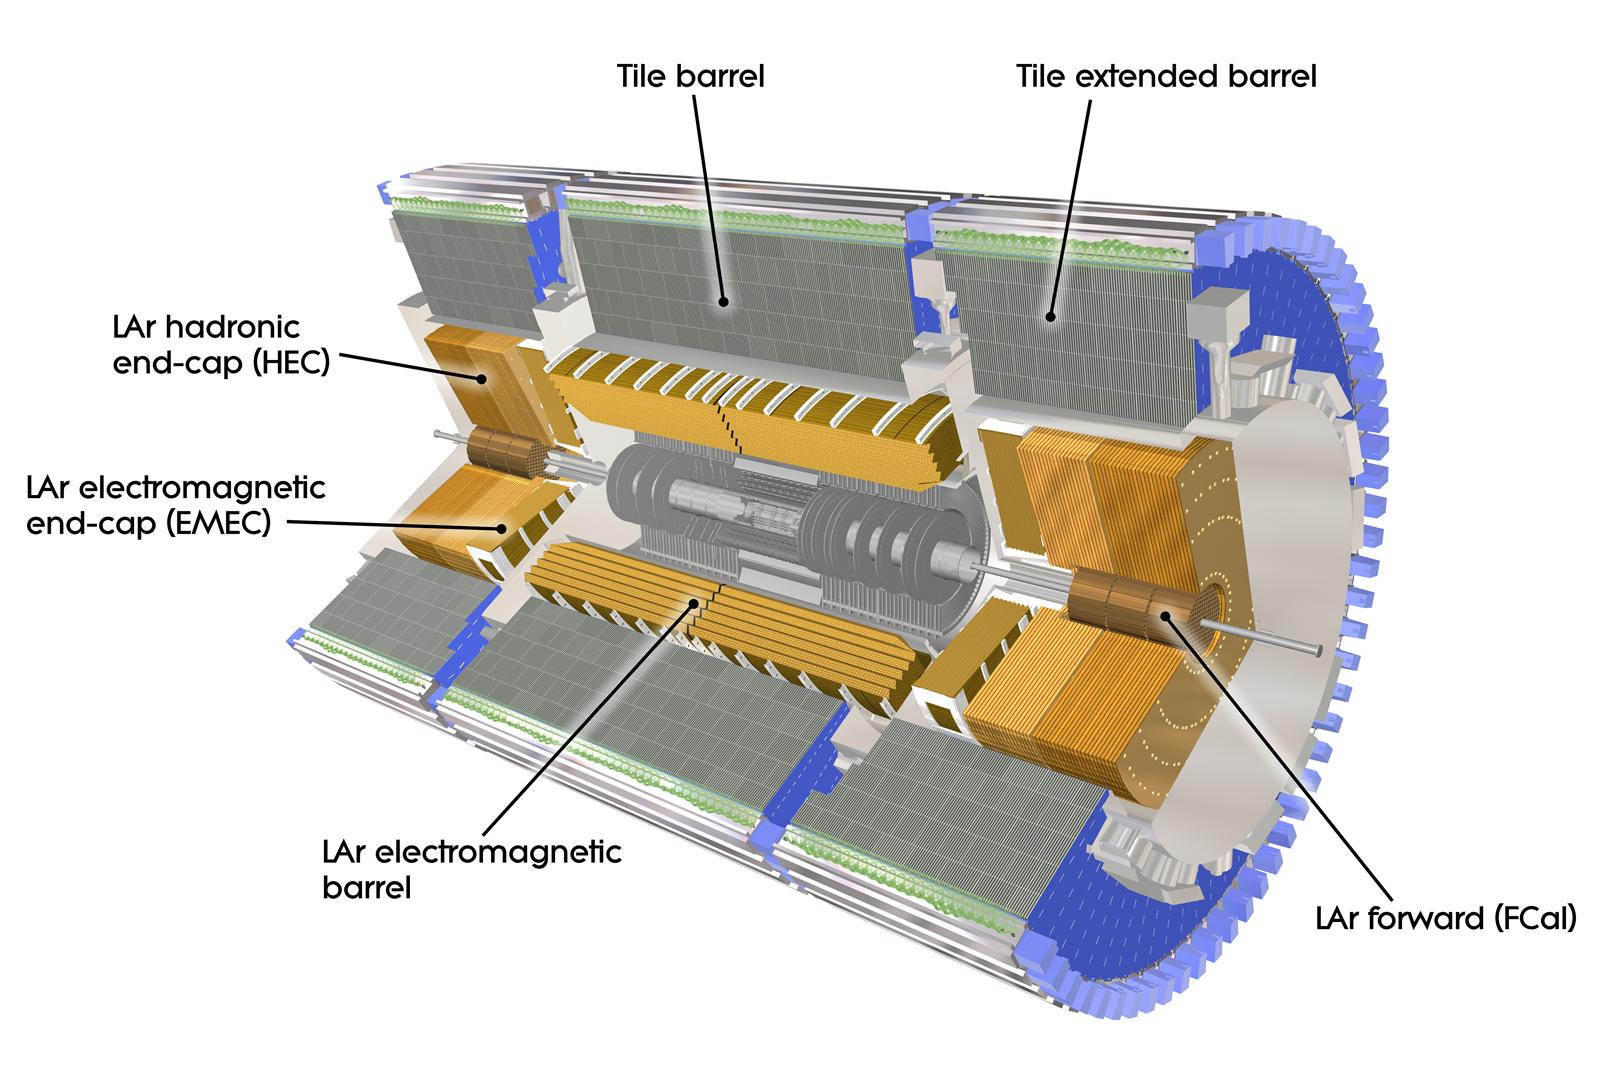
\includegraphics[width=\textwidth]{data/photo/calorimeter_whole.jpg}
\caption{whole calorimeter \cite{calorimeter_whole}}
\label{fig:calorimeter_whole}
\end{figure}

\subsubsection{Electromagnetic calorimeter}

\subsubsection{Hardronic calorimeter}

\subsection{Muon Spectrometer}
\begin{figure}
\centering
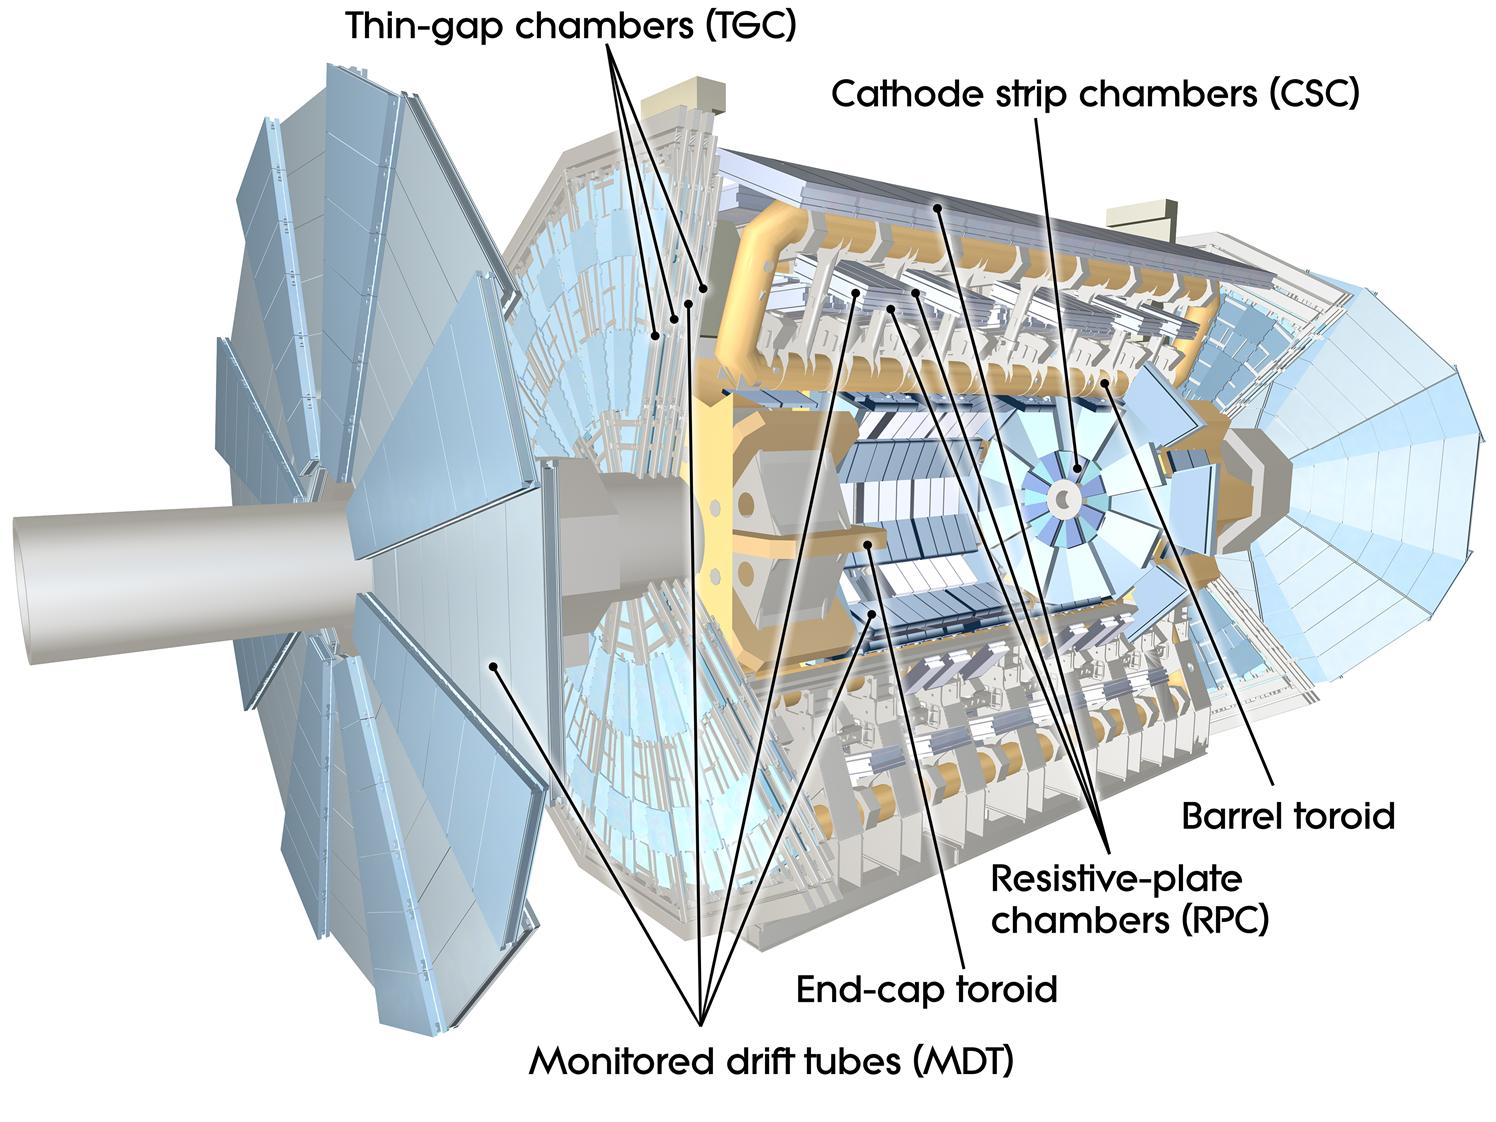
\includegraphics[width=\textwidth]{data/photo/muon_spectrometer.jpg}
\caption{muon spectrometer \cite{muon_spectrometer}}
\label{fig:muon_spectrometer}
\end{figure}

%************************************************
\chapter{Dataset inputs and event selection}
\label{ch:event}
%************************************************

\section{Dataset inputs}
This chapter describes the dataset used in this analysis.
The dataset contains the data samples and Monte-Carlo(MC) simulated sample.
All dataset are SUSY2 DxAOD derivations, which aim for 2 or 3 leptons search.

\subsection{Data samples}
We use 2015 (periods D-H and J) and 2016 (periods A-L, I, K and L) $pp$-collisions data samples, at $\sqrt s=13$ TeV.
Only events in good condition are used, where LHC beams were stable and all ATLAS detectors were in good state.
These good events are summarised in the Good Run Lists.
The two Good Run Lists (GRL) in 2015 and 2016 data are shown the section \ref{sec:List_Data}.
The integrated luminosities in 2015 and 2106 are $3.21$ fb$^{-1}$ and $32.86$ fb$^{-1}$ respectively, with relative error 2.1\%.
The list of data samples used in this analysis is shown the section \ref{sec:List_Data}.

\subsection{MC samples}
\subsubsection{SM background}
All MC samples are mc15c samples with offline release 20.7.
All the background MC samples used in this analysis for each process are shown in the section \ref{sec:MCBG} in appendix.
Each sample has its cross section, k-factor, generator efficiency and its equivalent integrated luminosity.
Some samples may overlap with each other.

\paragraph{$\bf t\bar{t}$ and single top}
The simulated events are generated by the {\sc POWHEG} generator, and the CT10 PDF set is used.
{\sc Pythia6} is also used for the parton shower model, with the {\sc Perugia} 2012 tune.
The mass of the top quark is assumed to be 172.5 GeV.
The $t\bar{t}$ samples are normalized to the next-to-next-to-leading order of cross section, while the single top samples are normalized to the next-to-leading order of cross section.

\paragraph{\bf W+jets and Z+jets}
The simulated events are generated by the {\sc SHERPA} v2.2.1.
The matrix elements are calculated at the next-to-leading order for up to two partons, and at the leading order for up to four partons, by using the {\sc Comix} and {\sc OpenLoops} generators.
The samples are normalized to the next-to-next-to-leading order QCD cross section.
The files are separated according to the $p_T$ of the vector boson and the presence of $b$-jet and $c$-jets.

\paragraph{\bf Diboson}
The processes with four charged leptons ($\ell \ell \ell \ell$), three charged leptons and one neutrino ($\ell \ell \ell \nu$), and two charged leptons and two neutrinos ($\ell \ell \nu \nu$) are simulated by the {\sc SHERPA} v2.2.1 generator.
Diboson $WW$, $WZ$ and $ZZ$ processes with four or six electroweak vertices are also used.

\paragraph{\bf Triboson}
The triboson processes $WWW$, $WWZ$, $WZZ$ and $ZZZ$ with up to six charged leptons are simulated by the {\sc SHERPA} v2.2.1 generator.

\paragraph{\bf ttV}
The processes $ttW$, $ttZ$, $ttWW$ and $ttWZ$ are simulated by {\sc MadGraph} v2.2.2 at the leading-order, with {\sc Pythia} for the parton shower model.

\paragraph{\bf Higgs}
The $WH$ and $ZH$ processes are generated by using {\sc Pythia} 8 generator, and the {\sc A14} set of tuned parameters is used together with the {\sc NNPDF23LO} PDF set.
The $ttH$ processes are generated by using {\sc Mcatnlo} generator, interfaced with {\sc Herwigpp}.
The CT10 PDF tuning is used along with the CTEQ6L1-UE-EE-5 tuning of parton shower.

\subsubsection{Signal}
The signal MC samples simulate the signal process $\tilde{\chi}_1^\pm \tilde{\chi}_2^0 \rightarrow W(\ell\nu)h$.
They are generated by the {\sc MadGraph} v2.2.3, calculated at the leading-order matrix elements with up to two extra partons.
{\sc Pythia} version 8.186 and the A14 tune are also used for the modelling of the SUSY decay chain, parton showering and hadronization.
Parton luminosities are provided by the NNPDF23LO PDF set.
Table \ref{table:signal} shows the list of signal samples used in this analysis, with different hypothesized masses point ($m_{\tilde{\chi}_1^\pm , \tilde{\chi}_2^0}$, $m_{\tilde{\chi}_1^0}$).
These signal samples have been applied a selection that at least 2 leptons with $p_{T} >$ 7 GeV is required.
The efficiencies due to this selection are applied and also shown in the table.

\section{Pre-selection and event cleaning}
\label{event_cleaning}
The following pre-selections on the events are applied to reject background which did not come from the proton-proton collision and to ensure that the detector was working properly.

\begin{itemize}
\item \textbf{Good Run List} The events need to pass the good run list. (For data only)
\item \textbf{LAr/Tile/SCT error} Events with data integrity errors in the SCT detector and the LAr and Tile calorimeter are removed. (For data only)
\item \textbf{Primary Vertex} The events need to have a primary vertex, which is defined as the one with the largest $\sum p_{T}^{2}$ of tracks, and has at least two tracks.
\item \textbf{Cosmic Muon Veto} The events with cosmic muons need to be removed. The track of cosmic muon is identified by large impact parameters with respect to the primary vertex, with the condition that $|z_{0}^{PV}|>1$ mm or $|d_{0}^{PV}|>0.2$ mm.
\item \textbf{Bad Muon Veto} The events with bad muons that does not come from the proton-proton collision need to be removed. The bad muon is identified by a large relative error in the ratio of electric charge to momentum ($q/p$), with the condition that $\sigma(q/p) / |q/p| > 0.2$, or by the ``Bad" quality by the recommendation of the Muon CP group.
\item \textbf{Bad Jet Veto} The events with bad jets that does not come from the proton-proton collision need to be removed. A jet with $p_{T}<$ 20 GeV or with the ``LooseBad" quality by the recommendation of the Jet/$E_T^{\text{miss}}$ group is identified as a bad jet.
\item \textbf{Trigger Selection} The events need to pass at least one trigger in the trigger list, described in section \ref{sec:trigger}.
\item \textbf{Exactly 2 baseline leptons} The events which have exactly 2 baseline leptons are selected. The definition of baseline electron and muon are described in section \ref{sec:object}. ``The two leptons" mentioned in the later chapters refer to these 2 baseline leptons. These two leptons are indexed in the descending order by their $p_T$. The lepton with larger $p_T$ is called the leading lepton ($\ell_1$), and the lepton with smaller $p_T$ is called the sub-leading lepton($\ell_2$).
\end{itemize}

\section{Trigger strategy}
\label{sec:trigger}
The time-spacing between two adjacent bunches is 25 ns, and equivalently the frequency is 40 MHz.
Because not all the collisions will be our interested events, and it is also infeasible to store all the events generated by the LHC to the permanent storage, the trigger strategy is used.
The trigger system accepts and rejects the events immediately after the data is taken.
The Level 1 trigger system filters the events from 40 MHz to 100 kHz.
The High Level trigger (HLT) system uses the output from the Level 1 trigger system, and further filters the events from 100 kHz to 1 kHz.

In our analysis, the single lepton trigger and di-lepton trigger was used. Table \ref{tab:single_trigger} and \ref{tab:dilepton_trigger} show the list of triggers used in this analysis.

\begin{table}[htbp]
\begin{center}
\begin{tabular}{|c|c|c|}
\hline
& \textbf{Single electron} & \textbf{Single muon}\\
\hline
\hline
2015 & \texttt{HLT\_e24\_lhmedium\_L1EM20VH} & \texttt{HLT\_mu20\_iloose\_L1MU15}\\
& \texttt{HLT\_e60\_lhmedium}           & \texttt{HLT\_mu40}\\
& \texttt{HLT\_e120\_lhloose}           & \\
\hline
2016 & \texttt{HLT\_e26\_lhtight\_nod0\_ivarloose} & \texttt{HLT\_mu26\_imedium}\\
& \texttt{HLT\_e60\_lhmedium\_nod0}          & \texttt{HLT\_mu50}\\
& \texttt{HLT\_e140\_lhloose\_nod0}          & \\
\hline
\end{tabular}
\end{center}
\caption{List of the single lepton triggers used in this analysis.}
\label{tab:single_trigger}
\end{table}

\begin{table}[htbp]
\begin{center}
\begin{tabular}{|c|c|c|c|}
\hline
& \textbf{Di-electron} & \textbf{Di-muon} & \textbf{Electron-muon}\\
\hline
\hline
2015 & \texttt{HLT\_2e12\_lhloose\_L12EM10VH} & \texttt{HLT\_mu18\_mu8noL1} & \texttt{HLT\_e17\_lhloose\_mu14}\\
     &                                        &                             & \texttt{HLT\_e7\_lhmedium\_mu24}\\
\hline
2016 & \texttt{HLT\_2e17\_lhvloose\_nod0}     & \texttt{HLT\_mu22\_mu8noL1} & \texttt{HLT\_e17\_lhloose\_nod0\_mu14}\\
     &                                        &                             & \texttt{HLT\_e7\_lhmedium\_nod0\_mu24}\\
\hline
\end{tabular}
\end{center}
\caption{List of the di-lepton triggers used in this analysis.}
\label{tab:dilepton_trigger}
\end{table}

\section{Object definitions}
\label{sec:object}
The object definitions are based on \texttt{SUSYTools-00-08-60} and analysis release \texttt{Base,2.4.31}, and their associated performance packages.

\subsection{Elections}
Electrons are reconstructed by using the recommendations from the egamma group and need to be inside the region $|\eta^{\text{cluster}}|<2.47$.
The baseline electrons are identified by the \texttt{LooseAndBLayerLLH} quality criterion and have $p_T>10$ GeV.
The signal electrons must be baseline electrons and satisfy additional criteria.
At the signal level, the electron must satisfy the \texttt{MediumLLH} quality criterion and has $p_T>25$ GeV.
The working point for the isolation cut is \texttt{FixedCutTight}.
The requirement for the impact parameter is $|z_0 \cdot \sin (\theta)|< 0.5$ mm and $|d_0/\sigma(d_0)|<5$, recommended by the Tracking CP group.
To reduce the charge flip background, \texttt{ChargeIDSelector} is used with the working point \texttt{Medium} at 97\% efficiency.
The selections for baseline and signal electrons are summarised in table \ref{tab:lepdef}.

\subsection{Muons}
Muons are reconstructed by using the recommendation from the MCP group and requiring $|\eta|<2.4$.
The baseline muons are identified by the \texttt{Medium} quality criterion and have $p_T>10$ GeV.
The signal muons must be baseline muons and satisfy additional criteria.
The additional criteria are $p_T>25$ GeV and isolation cut with the working point \texttt{GradientLoose}.
The requirement for the impact parameter is $|z_0 \cdot \sin (\theta)|< 0.5$ mm and $|d_0/\sigma(d_0)|<3$, recommended by the Tracking CP group.
The selections for baseline and signal muons are summarised in table \ref{tab:lepdef}.

\begin{table}[htbp]
\begin{center}
\begin{tabular}{|l|c|c|}
\hline
& \textbf{Baseline Electron} & \textbf{Baseline Muon} \\
\hline
\hline
Acceptance     & $p_T > 10$ GeV, $|\eta^{\text{cluster}}| < 2.47$  & $p_T > 10$ GeV, $|\eta| < 2.4$ \\
\hline
Quality & LooseAndBLayerLLH & Medium \\
\hline
\hline
& \textbf{Signal Electron} & \textbf{Signal Muon} \\
\hline
\hline
Acceptance & $p_T > 25$GeV & $p_T > 25$ GeV \\
\hline
Quality & MediumLLH & Medium \\
\hline
Isolation Cut  & \texttt{FixedCutTight} & \texttt{GradientLoose} \\
\hline
Impact parameter & $|z_0 \cdot \sin (\theta)|< 0.5$ mm   & $|z_0 \cdot \sin (\theta)|< 0.5$ mm \\
& $|d_0/\sigma(d_0)|<5$ & $|d_0/\sigma(d_0)| < 3$\\
\hline
ChargeIDSelector & Medium at 97\% efficiency & - \\
\hline
\end{tabular}
\end{center}
\caption{Summary of the electron and muon selection criteria. The signal selection requirements are applied on top of the baseline criteria.}
\label{tab:lepdef}
\end{table}

\subsection{Jets}
The baseline jets are reconstructed by the anti-$k_t$ jet algorithm with the distance parameter $D = 0.4$.
The baseline must has $p_T > 20$ GeV and $|\eta| < 2.8$.
The signal jets are selected on top of the baseline jet, with additional criteria.
The signal jets need to further satisfy the Jet Vertex Tagger (JVT) cut that JVT$> 0.59$ if the jets have $p_T < 60$ GeV and $|\eta| < 2.4$.
The b-jets are signal jets with b-tag, by using the MV2c10 b-tagging algorithm with \texttt{FixedCut} working point which has b-jet efficiency 77\%.
The selections of jets are summarised in table \ref{tab:jetsdef}.

\begin{table}[htbp]
\begin{center}
\begin{tabular}{|l|c|}
\hline
\hline
& \textbf{Baseline Jet} \\
\hline
\hline
Collection     & AntiKt4EMTopo \\
\hline
Acceptance     & $p_T > 20$ GeV, $|\eta| < 2.8$ \\
\hline
\hline
& \textbf{Signal Jet} \\
\hline
\hline
Acceptance     & $p_T > 20$ GeV, $|\eta | < 2.8$ \\
\hline
Jet vertex tagger  &  \texttt{Medium} working point\\
&  JVT $> 0.59$ for $p_T < 60$ GeV and $|\eta| < 2.4$\\
\hline
\hline
& \textbf{B-Jet} \\
\hline
\hline
Acceptance     & $p_T > 20$ GeV, $|\eta| < 2.4$ \\
\hline
$b-$tagging algorithm &  MV2c10 algorithm \\
Working point & \texttt{FixedCut} with efficiency 77\% \\
\hline
\end{tabular}
\end{center}
\caption{Summary of the jet selection criteria.}
\label{tab:jetsdef}
\end{table}

\subsection{Missing transverse momentum}
Based on the conservation of transverse momentum, the total transverse momentum of the missing particles,  which were not detected by the detector, can be estimated by the total transverse momentum of particles which can be detected.
The missing transverse momentum (${\bf p}_T^{\text{miss}}$) is defined by the negative of the sum of transverse momentum of all electrons, muons, photons, jets and all other tracks associated with the primary vertex.
The calibrated electrons, muons, photons and jet objects are used as the inputs.
This missing transverse momentum can estimate the total transverse momentum of the missing neutrinos and hypothetical neutralinos.
The Missing transverse energy ($E_{T}^{\text{miss}}$) is defined by the magnitude of the missing transverse momentum ${\bf p}_T^{\text{miss}}$.

\subsection{Overlap removal}
\label{sec:overlapRemoval}
The overlap removal (OR) is performed with the baseline objects (electrons, muons and jets) and follows the default prescription provided in the \texttt{SUSYTools}.
The objects are removed in the following order.
\begin{enumerate}
\item If a jet is within $\Delta R= \sqrt{(\Delta \eta)^2 + (\Delta \phi)^2}=0.2$ of an electron:
\begin{itemize}
\item If the jet is not $b-$tagged, then the jet is removed. It mostly originates from the calorimeter energy deposits by the electron shower.
\item If the jet is $b-$tagged, then the electron is removed. It is more likely that it results from the semi-leptonic decays of $b-$quarks.
\end{itemize}
\item Electrons within $\Delta R=0.4$ of a jet are removed, in order to suppress electrons from semi-leptonic decays of $c$- and $b$-hadrons.
\item Muons within $\Delta R=0.4$ of a jet are removed, in order to suppress muons from semi-leptonic decays of $c$- and $b$-hadrons.
\item Any calo-tagged muons sharing the same ID track with an electron are removed.
\item Any electrons sharing the same ID track with the remaining muons are removed.
\end{enumerate}

%************************************************
\chapter{Signal regions}
\label{ch:SR}
%************************************************

A signal region (SR) is the region in which signals are rich and the background are small.
It is designed to search for the new particles.
In the analysis, two signal regions are defined, SRjet1 and SRjet23.
Number of signal jets in SRjet1 is 1, while number of signal jets in SRjet23 is 2 or 3.
The details of the definition of these two signal regions will be described in section \ref{sec:signal_region_optimization}.

\section{Discriminant variables}
The discriminant variables are designed to define the signal regions.
The discriminant variables are used to distinguish the signal events from the background events, by applying a cut on the discriminant variable.
The following are the discriminant variables used in this analysis.
\begin{itemize}
\item $n_{\text{jets}}$: Number of signal jets:
\item $n_{\text{b-jets}}$: Number of $b$-jets.
\item $p_T^1$: Transverse momentum of the leading lepton.
\item $p_T^2$: Transverse momentum of the sub-leading lepton.
\item $\Delta \eta_{ll}$:
The difference in pseudorapidity between the two leptons.
\begin{equation}
\Delta \eta_{ll} = |\eta_{1} - \eta_{2}|
\end{equation}
\item $m_{ll}$:
The invariant mass of the two leptons (i.e. the invariant mass of the 4-momentum sum of the two leptons).
\begin{align}
(m_{ll})^2 = (p_1 + p_2)^2
\end{align}
\item $E_{T}^{\text{miss}}$:
The magnitude of the missing transverse momentum.
\begin{equation}
E_{T}^{\text{miss}} = |{\bf p}_T^{\text{miss}}|
\end{equation}
\item $m_T$:
It is designed to reconstruct the mass of the W-boson.
It is calculated by using the transverse momentum of the leading lepton and the missing transverse momentum, defined by equation \ref{equ:mT_def}.
By using the approximation $|{\bf p}_T^1| > 10$ GeV $\gg m_1$ (0.511 MeV or 106 MeV) and hence $E_T^1 = \sqrt{ (m_1)^2 + |{\bf p}_T^1|^2 } \approx |{\bf p}_T^1| $, it can be approximated by $m_T = \sqrt{2p_T^1 E_T^{\text{miss}}(1-\cos{\Delta\phi})}$, where $\Delta\phi$ is the azimuthal angle between the leading lepton and the missing transverse momentum.
\begin{align}
(m_T)^2 &= ( E_T^1 + E_T^{\text{miss}} )^2 - |{\bf p}_T^1 + {\bf p}_T^{\text{miss}}|^2 \label{equ:mT_def}\\
& \approx (|{\bf p}_T^1| + |{\bf p}_T^{\text{miss}}|)^2 - |{\bf p}_T^1 + {\bf p}_T^{\text{miss}}|^2 \\
&= (p_T^1 +  p_T^{\text{miss}})^2 - ({\bf p}_T^1 + {\bf p}_T^{\text{miss}}) \cdot ({\bf p}_T^1 + {\bf p}_T^{\text{miss}}) \\
&= (p_T^1)^2 + (p_T^{\text{miss}})^2 + 2 p_T^1 p_T^{\text{miss}}
 - (p_T^1)^2 - (p_T^{\text{miss}})^2 - 2 {\bf p}_T^1  \cdot {\bf p}_T^{\text{miss}} \\
&= 2 p_T^1 p_T^{\text{miss}} - 2 {\bf p}_T^1  \cdot {\bf p}_T^{\text{miss}} \\
&= 2 p_T^1 p_T^{\text{miss}} - 2 p_T^1 p_T^{\text{miss}} \cos{\Delta\phi} \\
&= 2 p_T^1 p_T^{\text{miss}} ( 1 - \cos{\Delta\phi} ) \\
m_T &= \sqrt{ 2 p_T^1 E_T^{\text{miss}} ( 1 - \cos{\Delta\phi} ) } \label{equ:mT_approx}
\end{align}
\item $m_{\text{eff}}$:
Effective mass is defined as the sum of the transverse momenta of the two leptons, signal jets and the missing transverse energy.
\begin{align}
m_{\text{eff}} = p_T^1 + p_T^2 + E_T^{\text{miss}} + \sum_{\text {signal jets}} p_T
\end{align}
\item $m_{lj}$ or $m_{ljj}$:
$m_{lj}$ is for the case that $n_{\text{jets}} = 1$ (i.e. SRjet1), while $m_{ljj}$ is for the case that $n_{\text{jets}} = 2$ or $3$ (i.e. SRjet23).
It attempts to reconstruct the mass of the Higgs boson.
It is defined as the invariant mass of the leading jet (i.e. the jet with the highest $p_T$) for SRjet1 or the di-jet system (i.e. the sum of the two leading jets) for SRjet23, and the closest lepton to the jet system, where the measure of distance is $\Delta R = \sqrt{(\Delta\phi)^2 + (\Delta\eta)^2}$.
The details of the definition are shown below.

The 4-momentum of the jet system is defined as
\begin{align}
p_{\text{jet-system}} =
\left\{
\begin{array}{ll}
p_{\text{jet1}} &\text{ for SRjet1}\\
p_{\text{jet1}} + p_{\text{jet2}} &\text{ for SRjet23}
\end{array} \right.
\end{align}

The 4-momentum of the closest lepton is defined as
\begin{align}
p_{\text{closest-lepton}} =
\left\{
\begin{array}{ll}
p_{\text{lepton1}} &\text{ if } \Delta R(p_{\text{lepton1}},p_{\text{jet-system}}) \leq \Delta R(p_{\text{lepton2}},p_{\text{jet-system}}) \\
p_{\text{lepton2}} &\text{ if } \Delta R(p_{\text{lepton1}},p_{\text{jet-system}}) > \Delta R(p_{\text{lepton2}},p_{\text{jet-system}})
\end{array} \right.
\end{align}

$m_{lj}$ or $m_{ljj}$ is defined as the invariant mass of the 4-momentum sum of the closest lepton and the jet system.
\begin{align}
(m_{lj(j)})^2 = (p_{\text{closest-lepton}} + p_{\text{jet-system}})^2
\end{align}

\item $m_{T2}$:
The ``stransverse mass'' ($m_{T2}$) is designed to set a lower bound on the masses of the unseen pair of charginos $\tilde{\chi}_1^\pm$ and neutralinos $\tilde{\chi}_2^0$.
One side is for charginos $\tilde{\chi}_1^\pm$ and another side is for neutralinos $\tilde{\chi}_2^0$, as shown in figure \ref{fig:signal_feynman}.
They are both assumed to decay into one lepton that can be detected, and into neutralinos $\tilde{\chi}_1^0$ and neutrino that cannot be detected and hence they contribute to the missing transverse momentum.
The calculation of $m_{T2}$ uses the transverse momentum of the two leptons (i.e. ${\bf p}_T^1$ and ${\bf p}_T^2$) and the missing transverse momentum ${\bf p}_T^{\text{miss}}$ as the inputs.
It is defined by finding the minimum value over all possible transverse vectors ${\bf q}_T$, which is the trial missing transverse momentum on one side \cite{MT2}.
\begin{equation}
m_{T2} = \min_{{\bf q}_T} \Bigg[ \max \bigg( m_T( {\bf p}_T^1, {\bf q}_T ), m_T( {\bf p}_T^2, {\bf p}_T^{\text{miss}} - {\bf q}_T ) \bigg) \Bigg]
\end{equation}
Similar to equation \ref{equ:mT_approx}, the transverse mass of two transverse momenta $m_T( {\bf p}_T, {\bf q}_T )$ is defined as follows.
\begin{equation}
m_T( {\bf p}_T, {\bf q}_T ) = \sqrt{ 2 p_T q_T ( 1 - \cos{\Delta\phi} ) }
\end{equation}
where $\Delta\phi$ is the azimuthal angle between the two transverse momenta.
\end{itemize}

\section{Signal region optimization}
\label{sec:signal_region_optimization}
This section describes how the signal region is found and optimizied.
The goal of the optimization is to increase the number of signal events $N_s$ and decrease the number of background event $N_b$.
This study was done, before we look at the real data, and hence the MC samples were used for signal and background.
The signal significance Z for large $N_s$ and $N_b$ is defined by
\begin{equation}
Z = \frac{N_s}{\sqrt{N_b + N_s}}
\label{equ:simple_significance}
\end{equation}
It measures how well the signal region is.
The process of the signal region optimization is to increase the signal significance Z.
The signal significance can be interpreted as the variable $z = \frac{x-\mu}{\sigma}$ in the standard normal distribution.
The corresponding p-value can be interpreted as the probability that the excess in the number of signal events from the background event is just due to the statistical fluctuation.
By changing the cuts on different discriminant variables, the maximum signal significance can be obtained, and the corresponding optimal cuts are the definition of the signal region.

Equation \ref{equ:simple_significance} is only valid for large $N_s$ and $N_b$.
Because $N_s$ and $N_b$ are often small, another sophisticated formula for the signal significance was used.
Also, the systematic error and statistical error of $N_b$ need to be taken account.
A fixed systematic error 25\% is used, and the total relative error $\sigma_b$ is the sum of systematic and statistical error in quadrature.
\begin{equation}
\sigma_b = \sqrt{(25\%)^2 + (\frac{\Delta N_b}{N_b})^2}
\end{equation}
where $\Delta N_b$ is the statistical error of $N_b$.
The signal significance is calculated by using the function \texttt{NumberCountingUtils::BinomialExpZ} provided in \texttt{RooStats}.
\begin{equation}
Z = \text{BinomialExpZ}(N_s,N_b,\sigma_b)
\label{equ:significance_def}
\end{equation}
This method basically calculates the signal significance Z with the corresponding p-value and probability for the following case.
A series of Bernoulli experiments is conducted with the number of trials $n = N_b + N_s + \frac{1}{\sigma_b ^2}$ and the probability of success of each trial $p = 1/(1 + 1/(N_b \sigma_b ^2))$ \cite{2-leptons-long}.
The corresponding p-value is the probability that the number of success is at least $N_b + N_s$.
The connection between these Bernoulli experiments and our analysis will not be explained here, but what is important is that the signal significance Z calculated by the equation \ref{equ:significance_def} is an approximation to our analysis. It is useful because it has the following properties.
\begin{itemize}
\item It is a continuous function. $N_b$ and $N_s$ can be non-integer. (cf. Poisson distribution)
\item It is a smooth function. It is convenient for finding the maximum value.
\item For large $N_b$ and $N_s$, it reduces to equation \ref{equ:simple_significance}.
\item It is fast to compute.
\end{itemize}
By using the equation \ref{equ:significance_def}, an approximately optimal signal region can be found.

\subsection{Pre-selection}
\label{sec:SR_pre-selection}
Before the optimization, the following pre-selections are applied, on top of the selections in section \ref{event_cleaning}.
\begin{itemize}
\item \textbf{Exactly 2 signal leptons} The events which have exactly 2 signal leptons are selected. This means that the two leptons must be signal leptons.
\item \textbf{Same sign} The electric charges of the two leptons have the same sign. This is what we are looking for, described in section \ref{sec:Wh_signal}.
\item \textbf{B-jet veto} To suppress the top background, the number of b-jets is 0.
\item \textbf{Number of jet} Similar to the Run 1 analysis, two signal regions are defined according to the number of signal jets. One signal region has 1 signal jet, called ``SRjet1'', and another has 2 or 3 signal jets, called ``SRjet23''.
\end{itemize}

\subsection{Samples}
As mentioned before, MC samples were used for estimating the expected $N_s$ and $N_b$ in the process of optimization.

For the signal, the mass point ($m_{\tilde{\chi}_1^\pm , \tilde{\chi}_2^0}$,$m_{\tilde{\chi}_1^0}$) = (225,75) was used for SRjet1, while the mass point ($m_{\tilde{\chi}_1^\pm , \tilde{\chi}_2^0}$,$m_{\tilde{\chi}_1^0}$) = (187.5,37.5) was used for SRjet23.

For the background, MC samples were used for diboson (WZ, WW and ZZ), ttV and rare processes (triboson, multi-top and Higgs).
Instead of using the corresponding MC samples, the fake lepton background is estimated by the matrix method as described in section \ref{sec:fake_background}, because the fake lepton background is the major background and the corresponding MC sample is not reliable.
The charge flip background estimated in section \ref{sec:charge_flip_background} was also used.
The plots after the pre-selection in section \ref{sec:SR_pre-selection}, but before the optimization, are shown in figures \ref{fig:SRjet1_pre-selection} and \ref{fig:SRjet23_pre-selection}.

\begin{figure}[htpb]
\centering
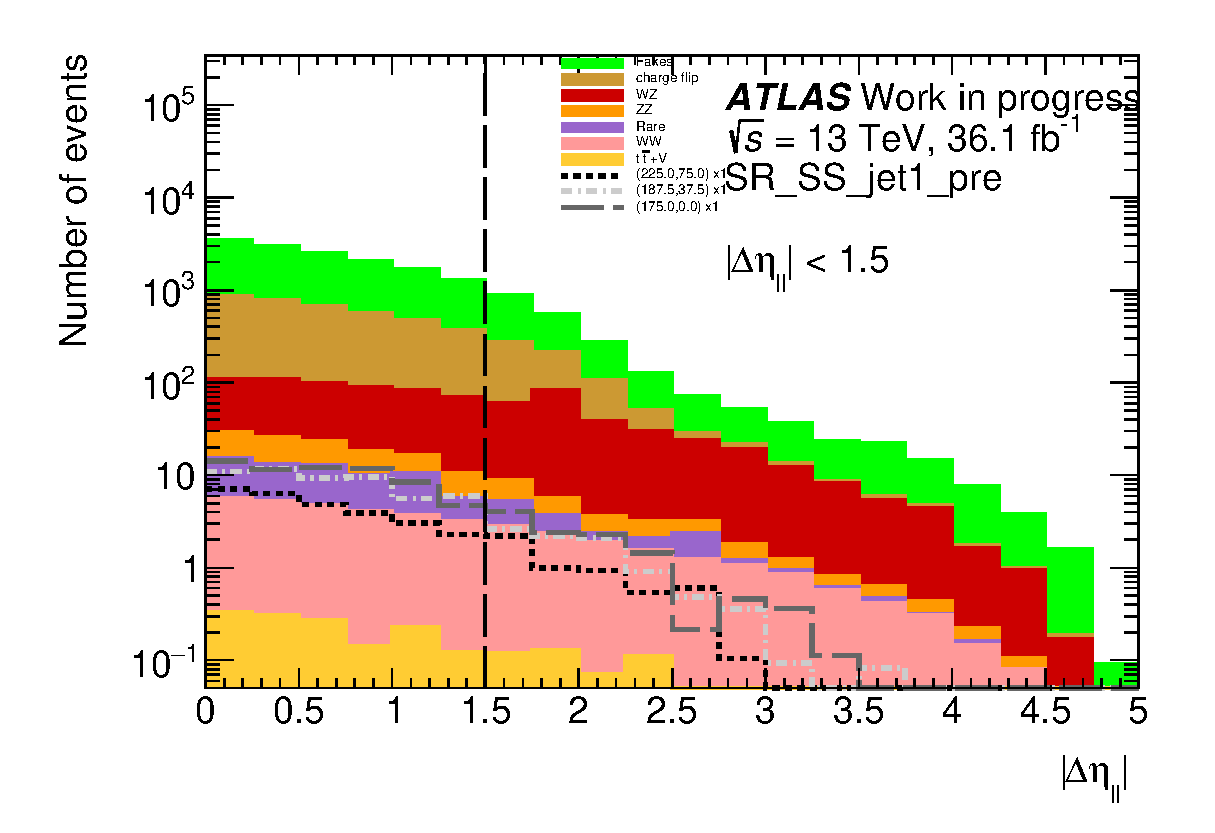
\includegraphics[width=0.45\linewidth]{data/plot/plot_SR/dEta_SR_SS_jet1_pre}
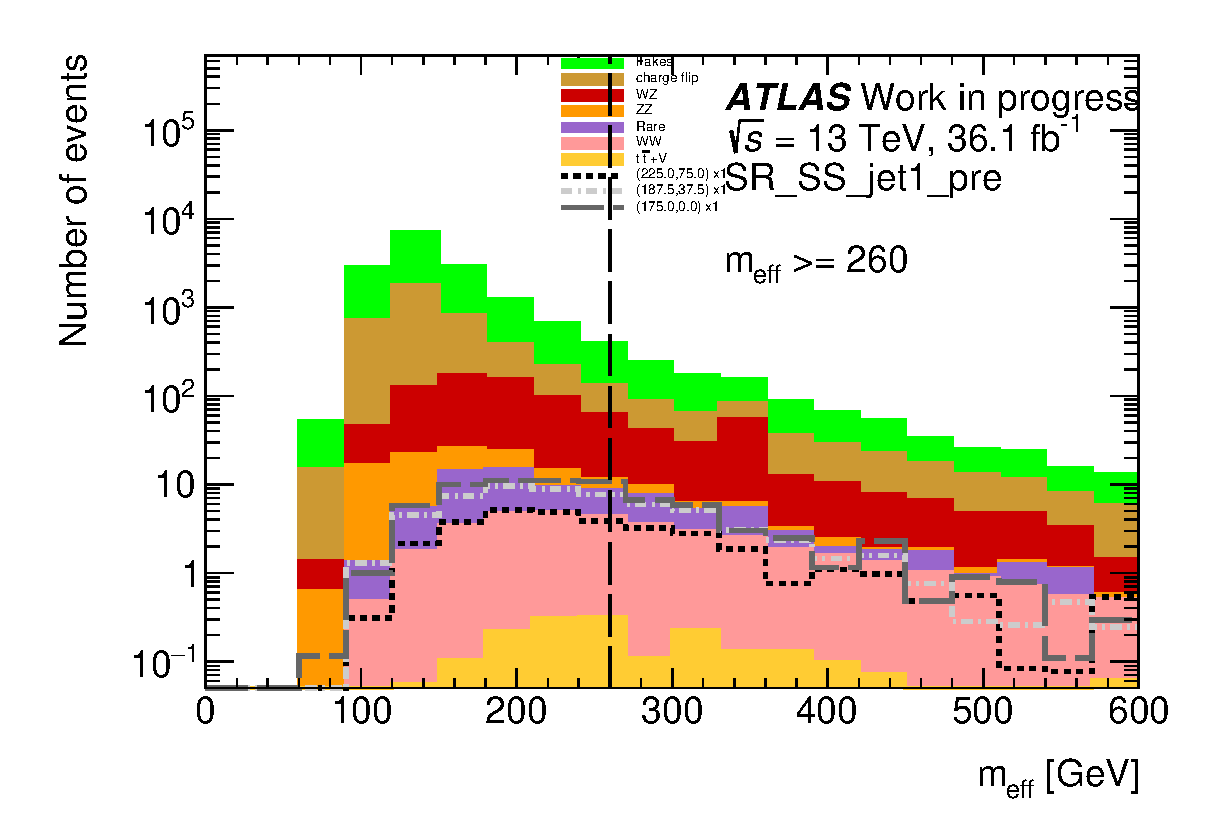
\includegraphics[width=0.45\linewidth]{data/plot/plot_SR/meff_SR_SS_jet1_pre}\\
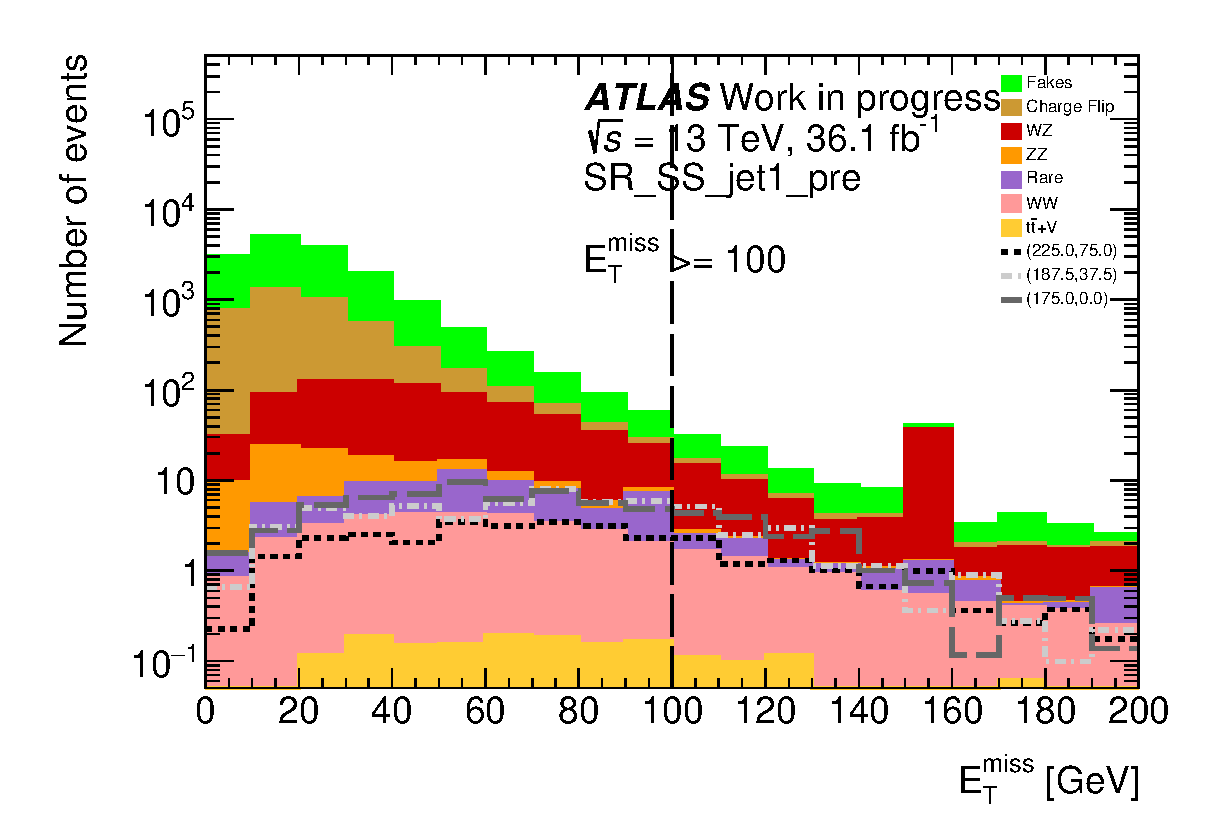
\includegraphics[width=0.45\linewidth]{data/plot/plot_SR/MET_SR_SS_jet1_pre}
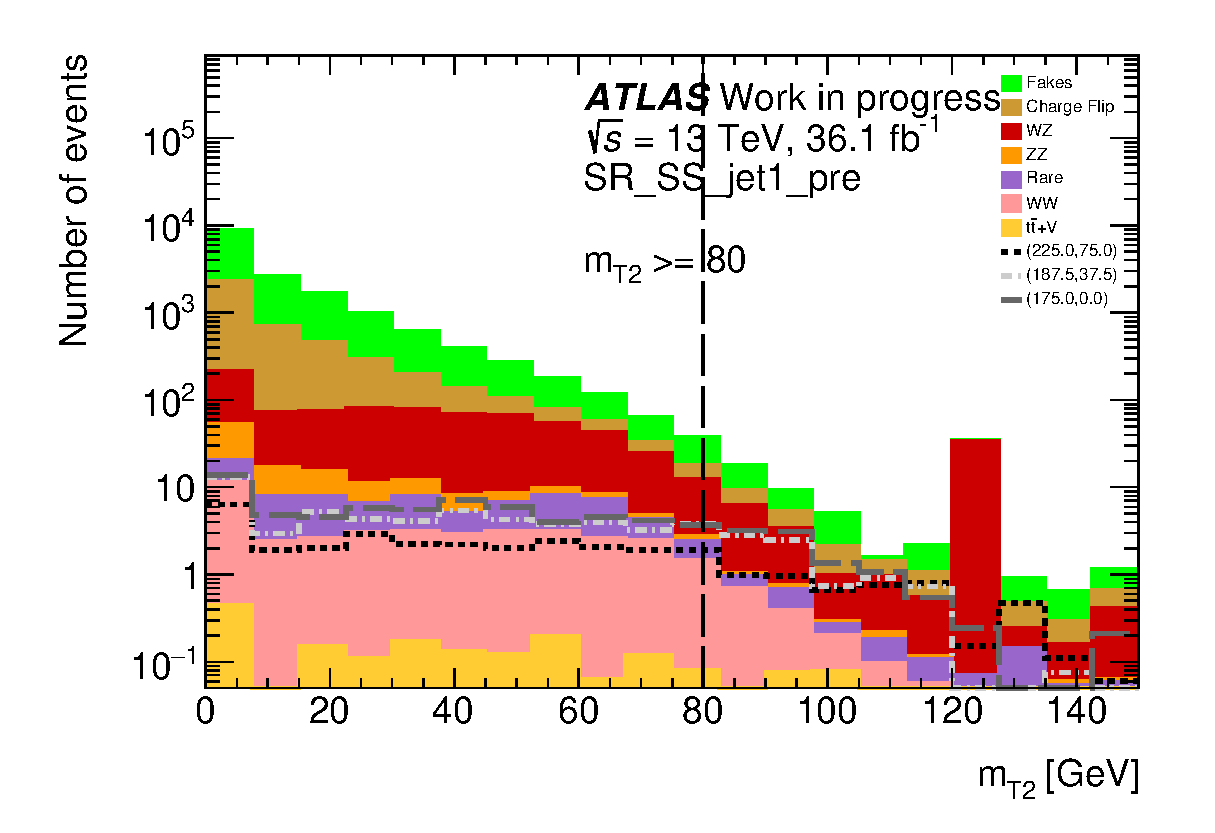
\includegraphics[width=0.45\linewidth]{data/plot/plot_SR/mTtwo_SR_SS_jet1_pre}\\
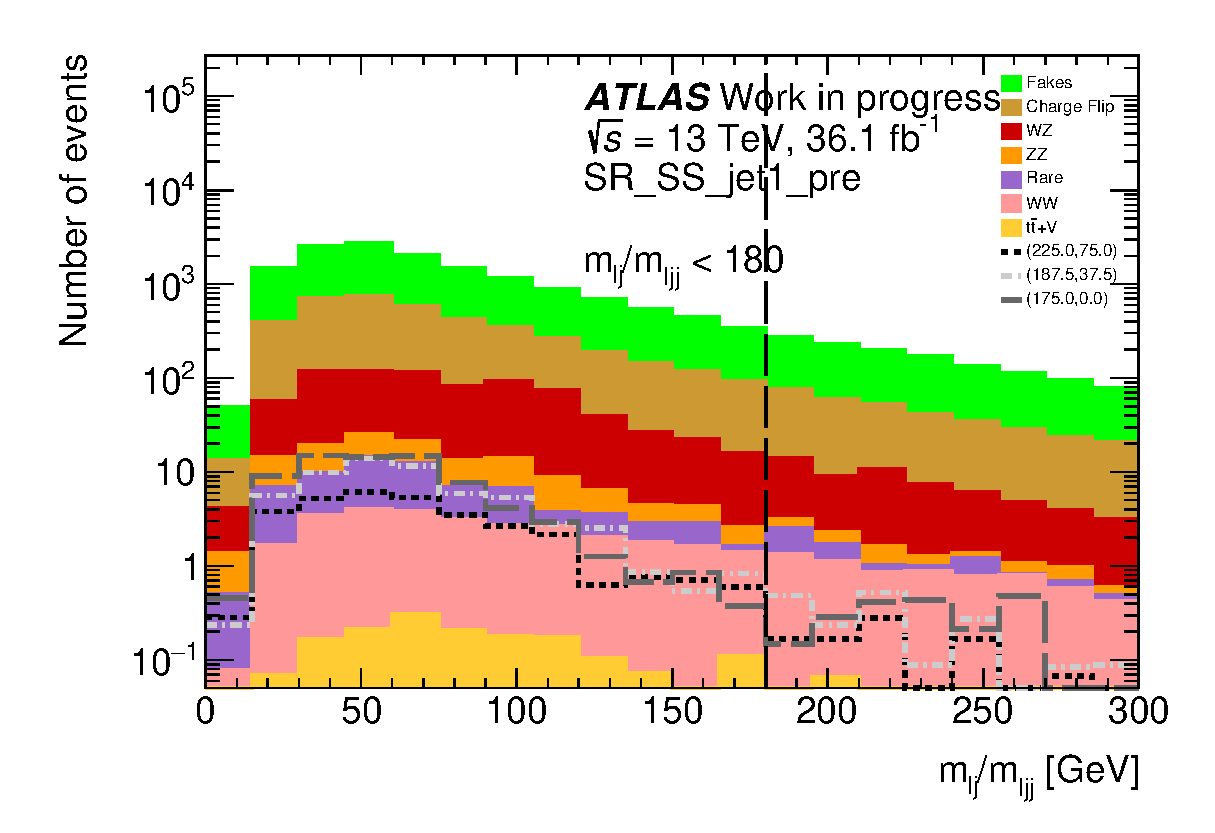
\includegraphics[width=0.45\linewidth]{data/plot/plot_SR/mlj_SR_SS_jet1_pre}
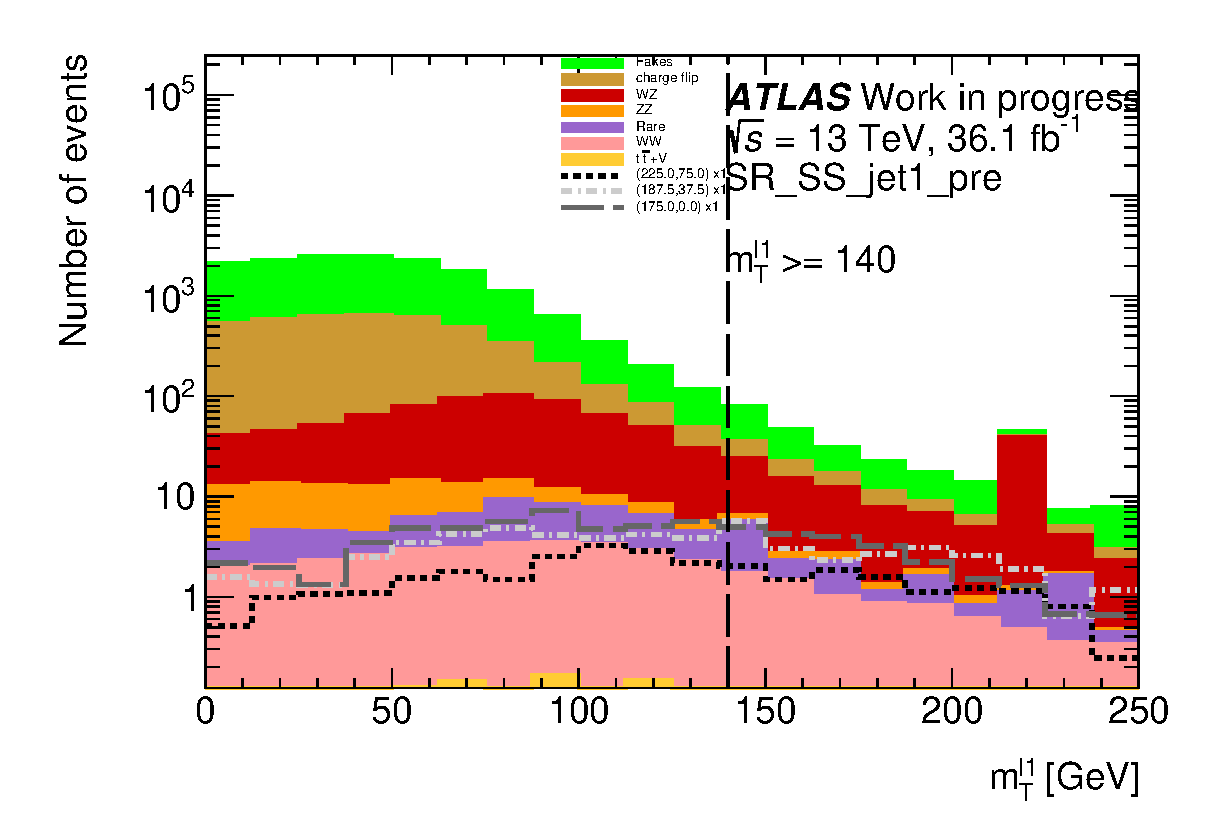
\includegraphics[width=0.45\linewidth]{data/plot/plot_SR/mt1_SR_SS_jet1_pre}\\
\caption{Distribution of the kinematic variables used for the optimization in SRjet1. The pre-selection has been applied.}
\label{fig:SRjet1_pre-selection}
\end{figure}

\begin{figure}[htpb]
\centering
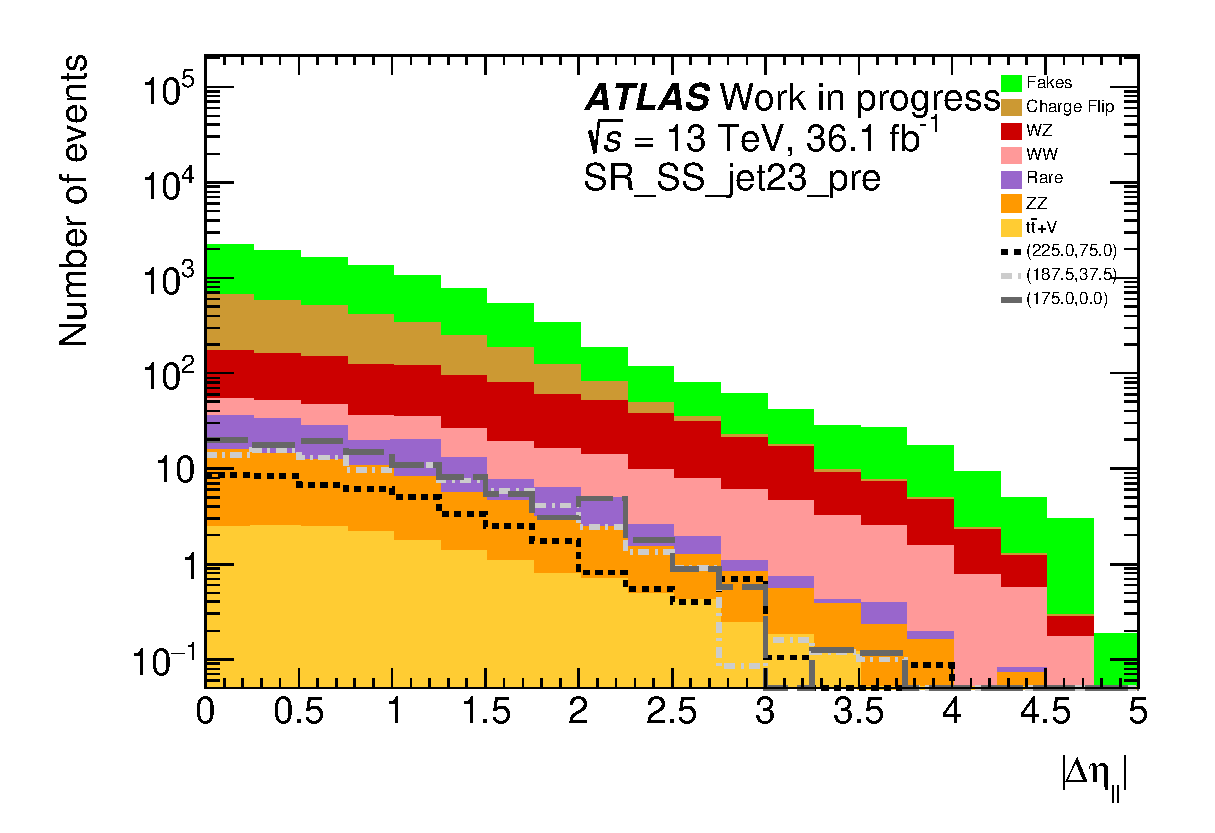
\includegraphics[width=0.45\linewidth]{data/plot/plot_SR/dEta_SR_SS_jet23_pre}
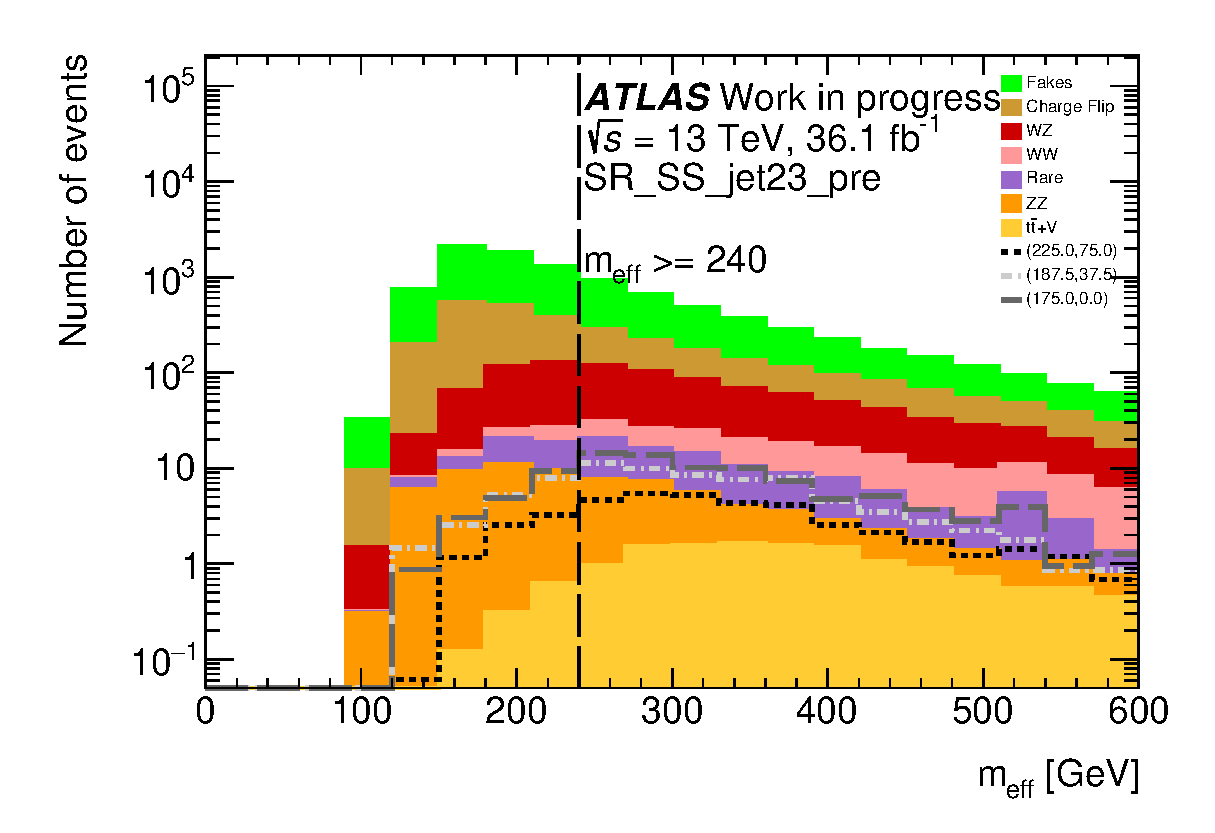
\includegraphics[width=0.45\linewidth]{data/plot/plot_SR/meff_SR_SS_jet23_pre}\\
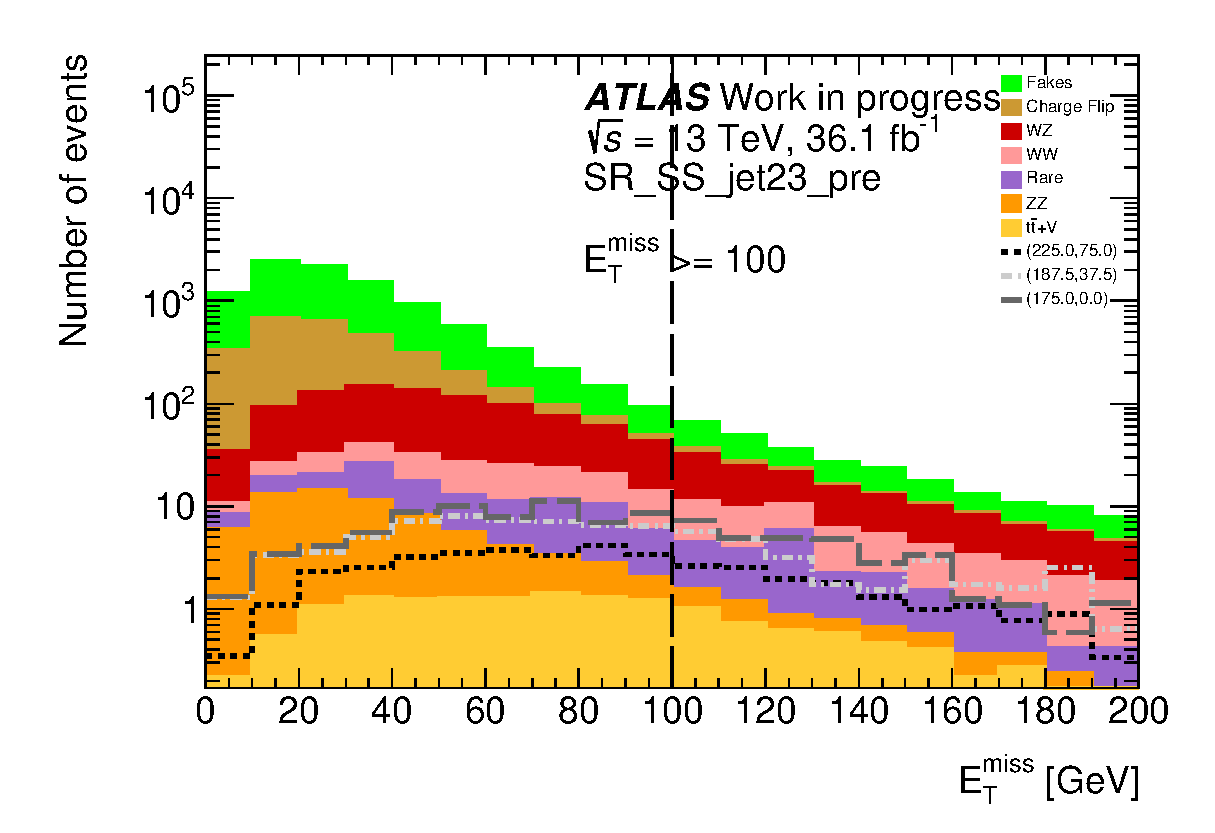
\includegraphics[width=0.45\linewidth]{data/plot/plot_SR/MET_SR_SS_jet23_pre}
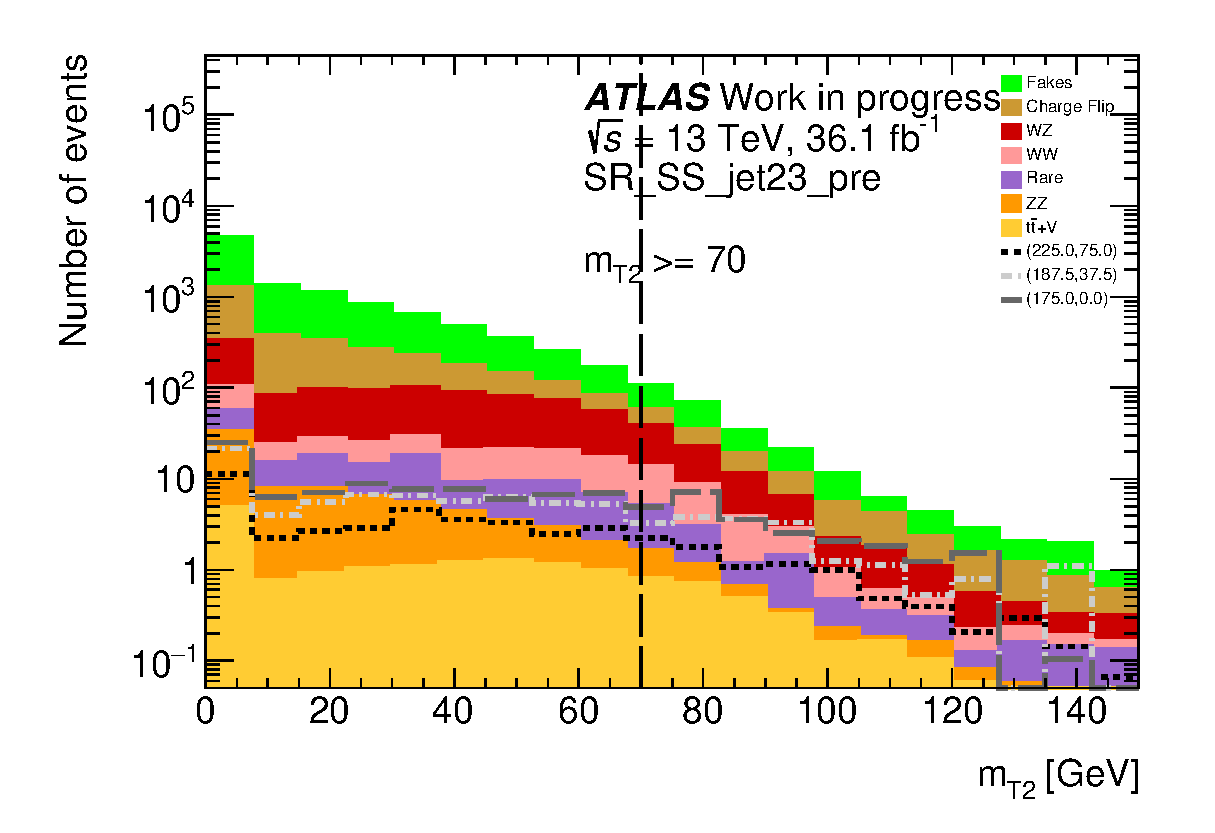
\includegraphics[width=0.45\linewidth]{data/plot/plot_SR/mTtwo_SR_SS_jet23_pre}\\
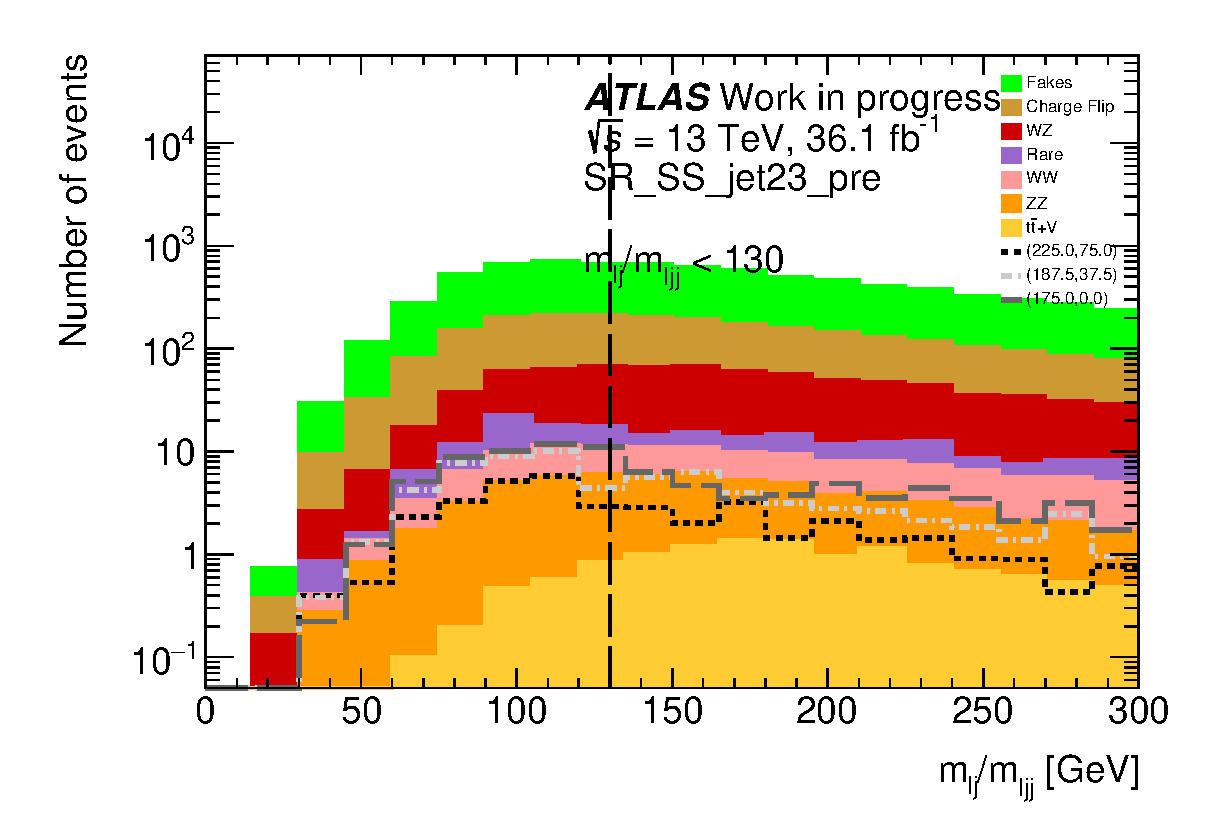
\includegraphics[width=0.45\linewidth]{data/plot/plot_SR/mlj_SR_SS_jet23_pre}
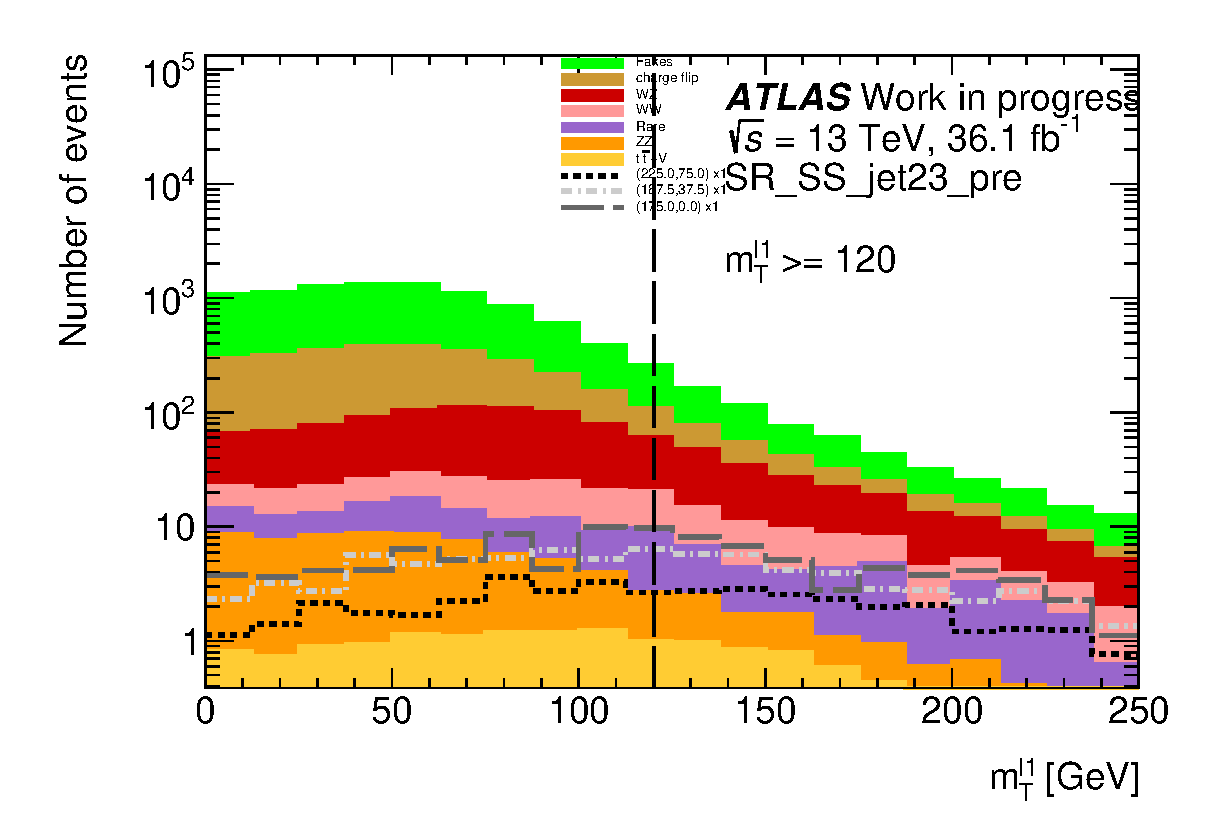
\includegraphics[width=0.45\linewidth]{data/plot/plot_SR/mt1_SR_SS_jet23_pre}\\
\caption{Distribution of the kinematic variables used for the optimization in SRjet23. The pre-selection has been applied.}
\label{fig:SRjet23_pre-selection}
\end{figure}

\subsection{Running for optimization}
Some constraints were applied during the process of optimization, in order to have enough statistics to have reliable estimation of $N_s$ and $N_b$.
\begin{itemize}
\item The yields (i.e. the sum of weighted events) for each process of background need to be positive, to have a reasonable and stable modelling of the background shape.
Also, the HistFitter requires the background need to have positive yields.
\item The diboson and ttV background have at least 10 unweighted events respectively, to have a reliable estimation for the main background processes from prompt leptons (i.e. not fake leptons).
\item For $E_T^{\text{miss}}$, $m_T$, $m_{\text{eff}}$ and $m_{T2}$, only lower cuts are applied.
\item For $\Delta \eta_{ll}$ and $m_{lj(j)}$, only upper cuts are applied.
\end{itemize}

The list of variables used is shown in the table \ref{tab:variables_optimization}.

\begin{table}[htbp]
\centering
\begin{tabular}{|c|c|}
\hline
Variable & direction of cut \\
\hline
\hline
$\Delta \eta_{ll}$ & upper cut \\
\hline
$E_T^{\text{miss}}$ & lower cut \\
\hline
$m_T$ & lower cut \\
\hline
$m_{\text{eff}}$ & lower cut \\
\hline
$m_{lj(j)}$ & upper cut \\
\hline
$m_{T2}$ & lower cut \\
\hline
\end{tabular}
\caption{Kinematic variables used in the optimization.}
\label{tab:variables_optimization}
\end{table}

\subsection{Results for optimization}
The final results for the definitions of the two signal regions are shown in table \ref{tab:SR_Def}.
The yields for different background and signal processes are shown in table \ref{tab:SRjet1_yields} and \ref{tab:SRjet23_yields}.
The N-1 plots for the discriminant variables are shown in figures \ref{fig:SRjet1_N1} and \ref{fig:SRjet23_N1}.
The N-1 plot means that all other SR selections are applied, except the selection for that variable.

\begin{table}[htpb]
\centering
\begin{tabular}{|c|c|c|}
\hline
Variable &  SRjet1 & SRjet23 \\ \hline
$\Delta\eta_{ll}$ & $\leq 1.5$ &  -- \\
$E_T^{\text{miss}}$ &  $\geq 100 $ GeV  & $\geq 100$ GeV\\
$m_T$ & $\geq 140$ GeV & $\geq 120$ GeV \\
$m_{\text{eff}}$ & $\geq 260$ GeV &  $\geq 240$ GeV\\
$m_{lj(j)}$ & $< 180$ GeV &  $< 130$ GeV\\
$m_{T2}$ & $\geq 80$ GeV&  $\geq 70$ GeV \\
\hline
\end{tabular}
\caption{Final SR definitions}
\label{tab:SR_Def}
\end{table}

\begin{table}[htpb]
\centering
\begin{tabular}{|c|c|c|}
\hline
& Number of events & Significance \\
\hline
\hline
Fakes & $3.295\pm0.819$ (24) & \\
\hline
WZ & $2.176\pm0.398$ (257) & \\
\hline
Charge Flip & $0.472\pm0.053$ (265) & \\
\hline
Rare & $0.444\pm0.111$ (56) & \\
\hline
WW & $0.166\pm0.023$ (67) & \\
\hline
$t\bar{t}+V$ & $0.125\pm0.046$ (36) & \\
\hline
ZZ & $0.055\pm0.028$ (31) & \\
\hline
\hline
Total BG & $6.733\pm0.921$ (736) & \\
\hline
\hline
(225.0,75.0) & $3.33\pm0.60$ (60) &$ \bf 0.74$\\
\hline
(187.5,37.5) & $3.77\pm0.95$ (31) &$0.86$\\
\hline
(175.0,0.0) & $4.29\pm0.73$ (36) &$0.98$\\
\hline
\end{tabular}
\caption{The yields in SRjet1. The unweighed event are also shown in parentheses.}
\label{tab:SRjet1_yields}
\end{table}

\begin{table}[htpb]
\centering
\begin{tabular}{|c|c|c|}
\hline
& Number of events & Significance \\
\hline
\hline
WZ & $1.849\pm0.273$ (319) & \\
\hline
Fakes & $1.765\pm0.709$ (20) & \\
\hline
Rare & $0.731\pm0.195$ (48) & \\
\hline
WW & $0.514\pm0.037$ (235) & \\
\hline
Charge Flip & $0.267\pm0.029$ (274) & \\
\hline
$t\bar{t}+V$ & $0.142\pm0.031$ (67) & \\
\hline
ZZ & $0.067\pm0.025$ (24) & \\
\hline
\hline
Total BG & $5.335\pm0.787$ (987) & \\
\hline
\hline
(225.0,75.0) & $2.35\pm0.34$ (58) &$0.57$\\
\hline
(187.5,37.5) & $4.72\pm0.74$ (47) &$\bf 1.26$\\
\hline
(175.0,0.0) & $8.60\pm1.51$ (58) &$2.24$\\
\hline
\end{tabular}
\caption{The yields in SRjet23. The unweighed event are also shown in parentheses.}
\label{tab:SRjet23_yields}
\end{table}

\begin{figure}[htpb]
\centering
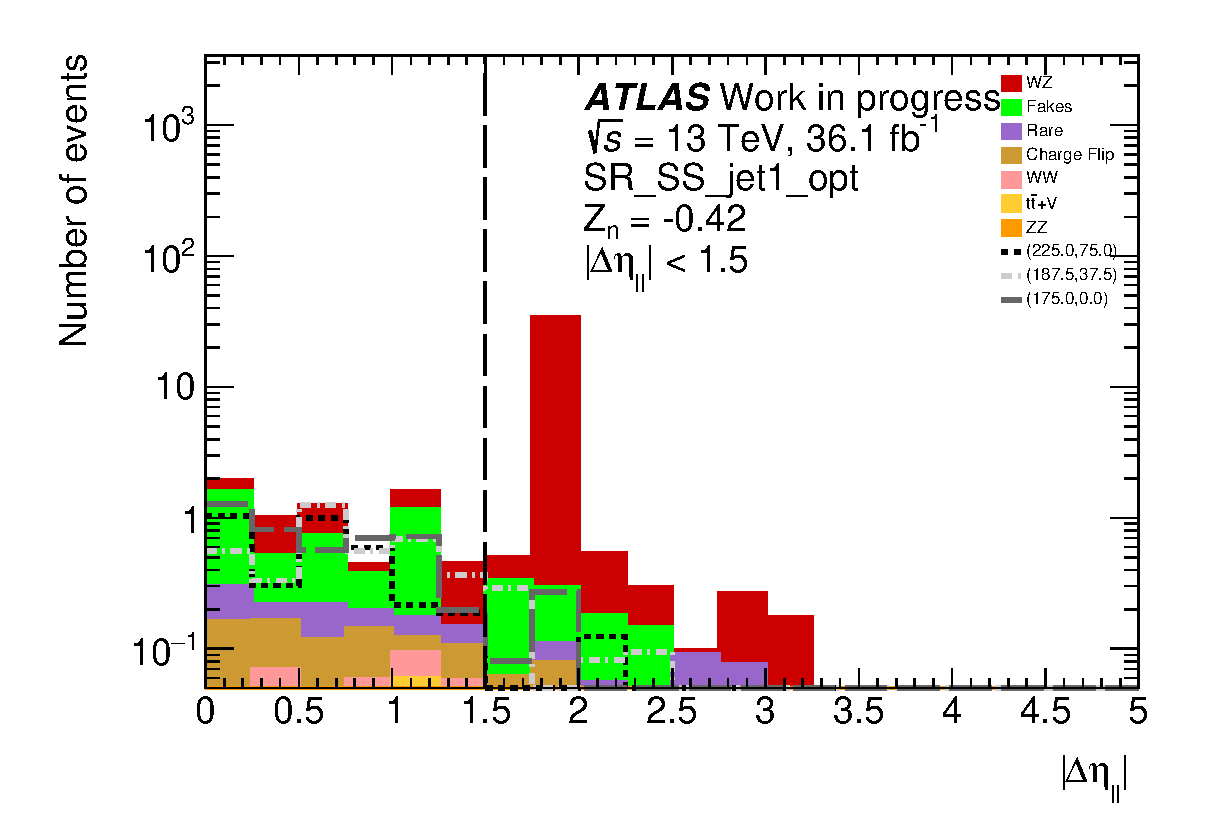
\includegraphics[width=0.45\linewidth]{data/plot/plot_SR/dEta_SR_SS_jet1_opt_0}
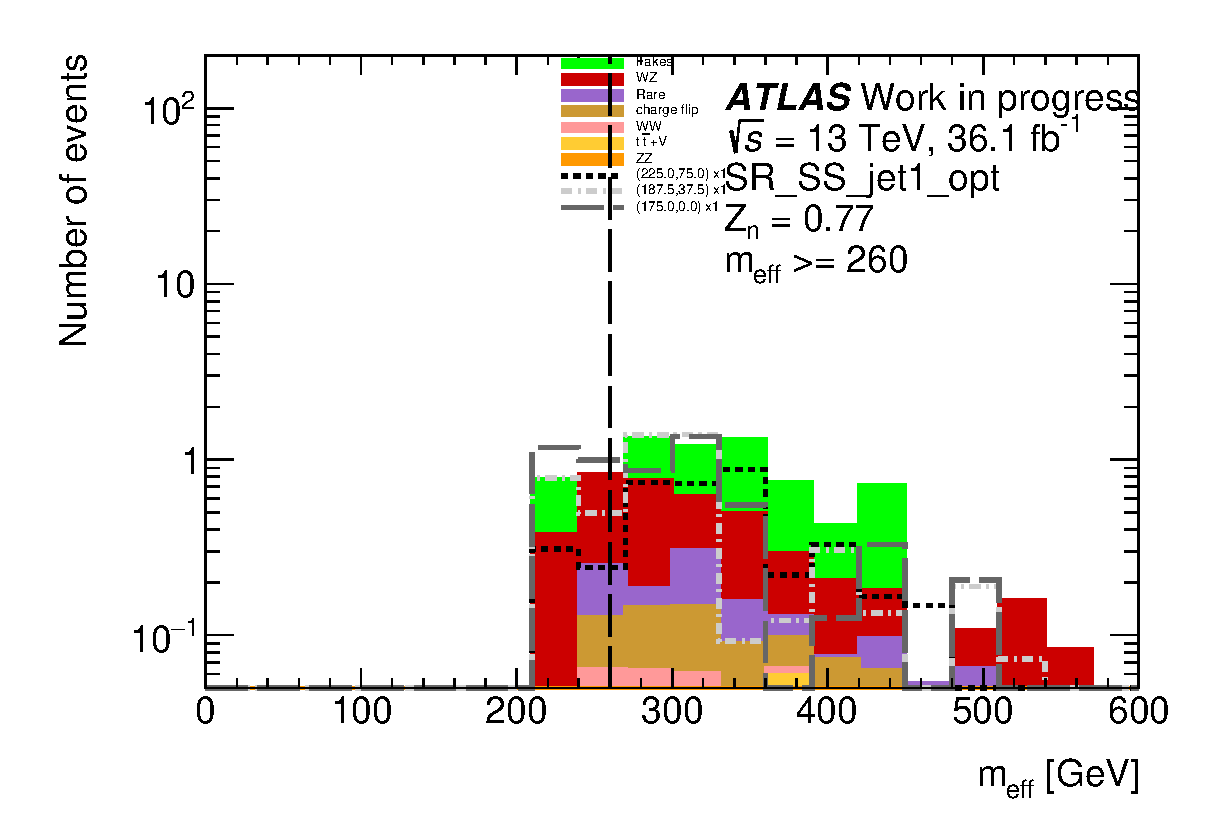
\includegraphics[width=0.45\linewidth]{data/plot/plot_SR/meff_SR_SS_jet1_opt_0}\\
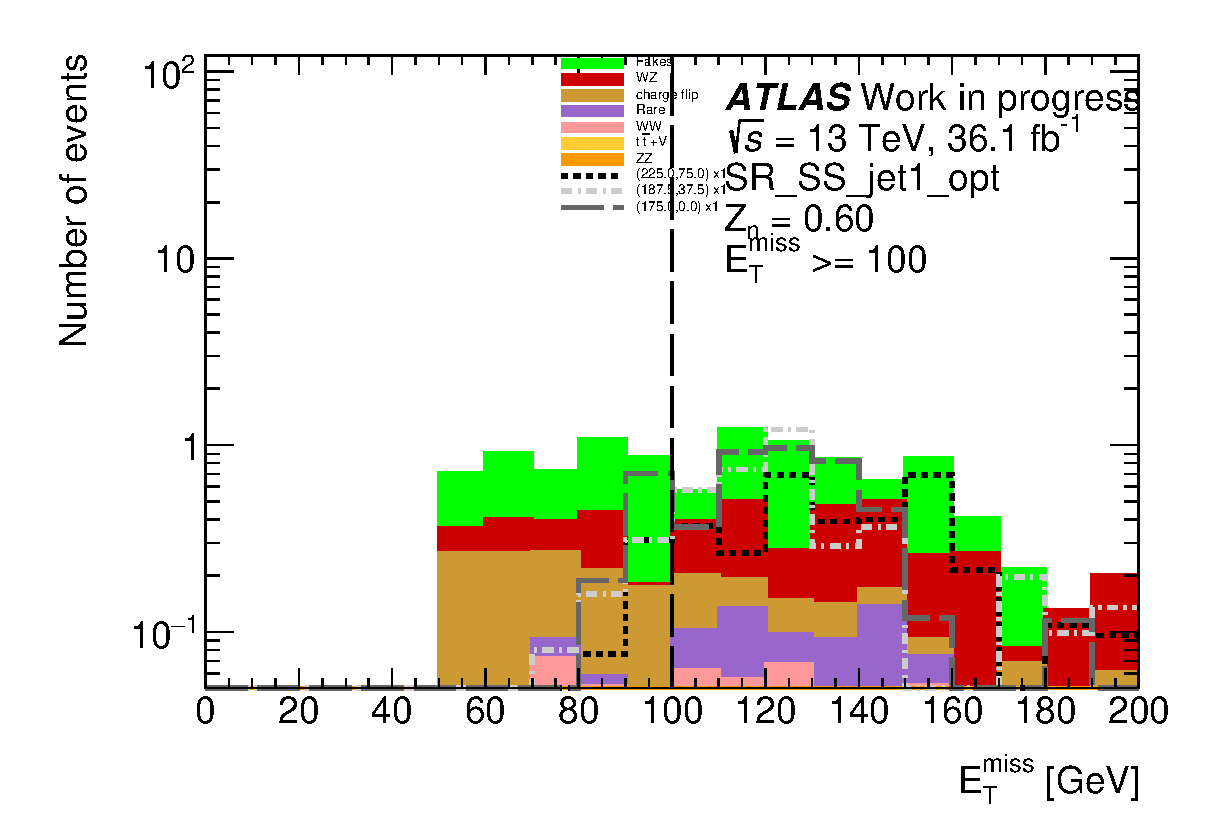
\includegraphics[width=0.45\linewidth]{data/plot/plot_SR/MET_SR_SS_jet1_opt_0}
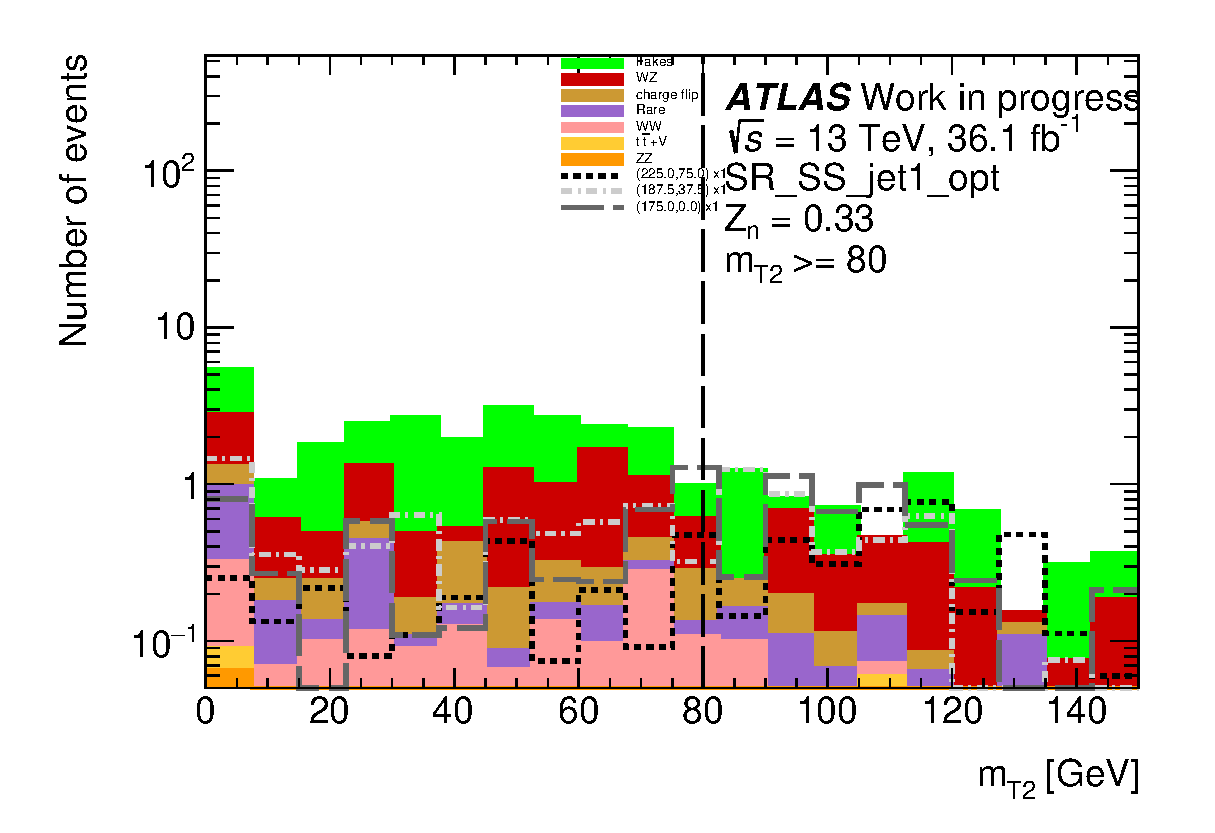
\includegraphics[width=0.45\linewidth]{data/plot/plot_SR/mTtwo_SR_SS_jet1_opt_0}\\
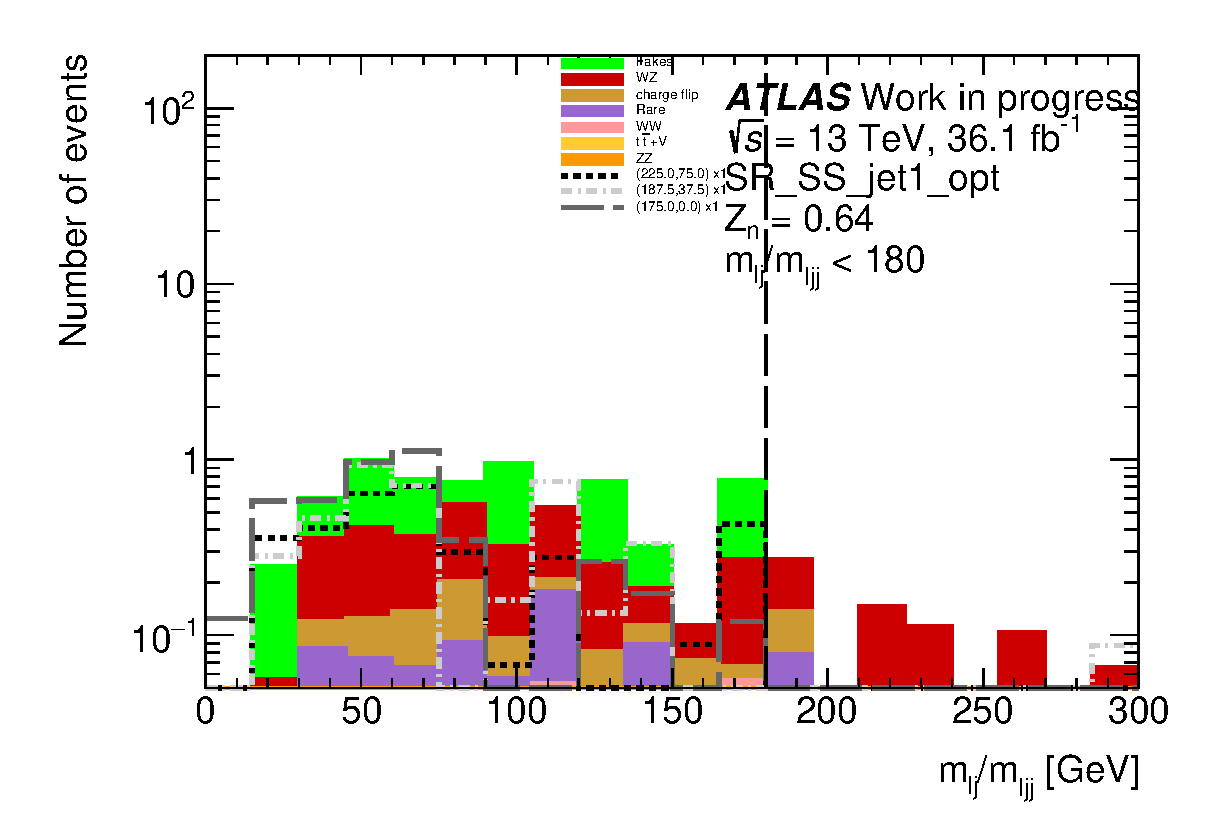
\includegraphics[width=0.45\linewidth]{data/plot/plot_SR/mlj_SR_SS_jet1_opt_0}
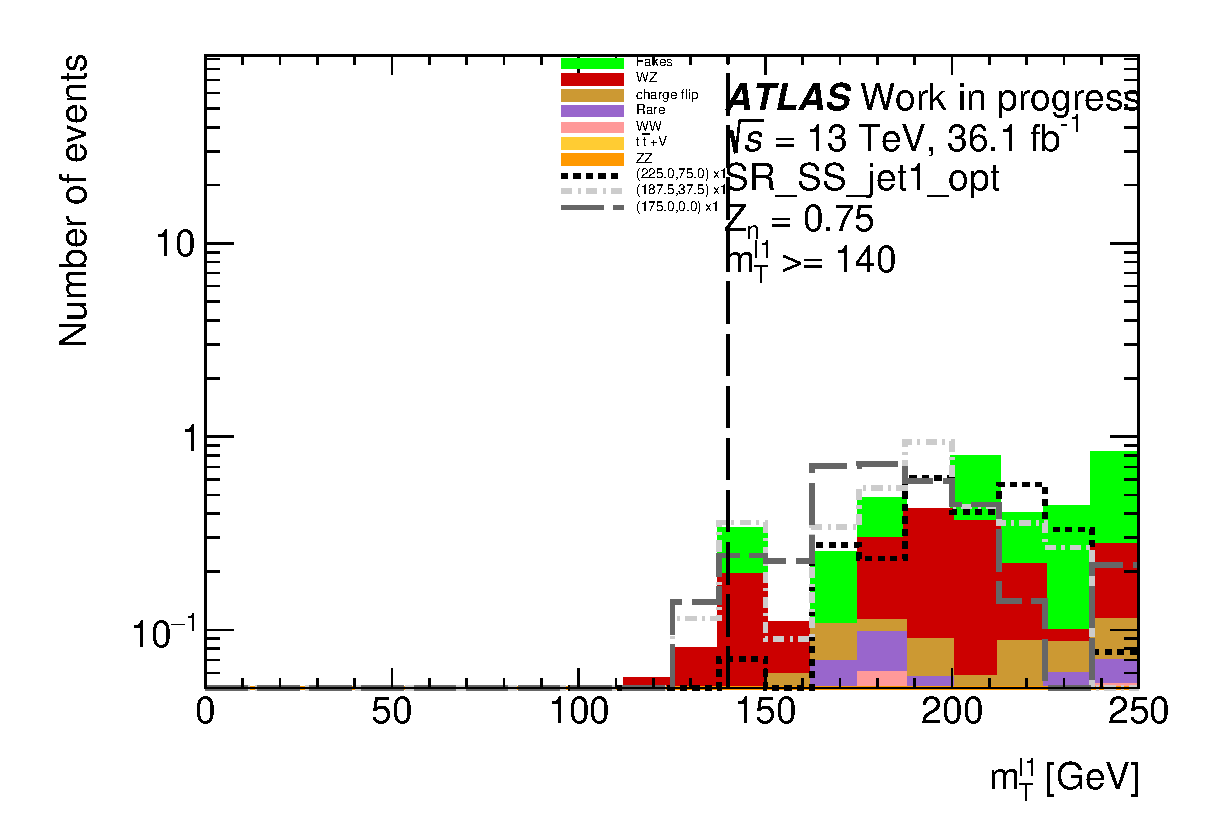
\includegraphics[width=0.45\linewidth]{data/plot/plot_SR/mt1_SR_SS_jet1_opt_0}\\
\caption{The N-1 plots for SRjet1.}
\label{fig:SRjet1_N1}
\end{figure}


\begin{figure}[htpb]
\centering
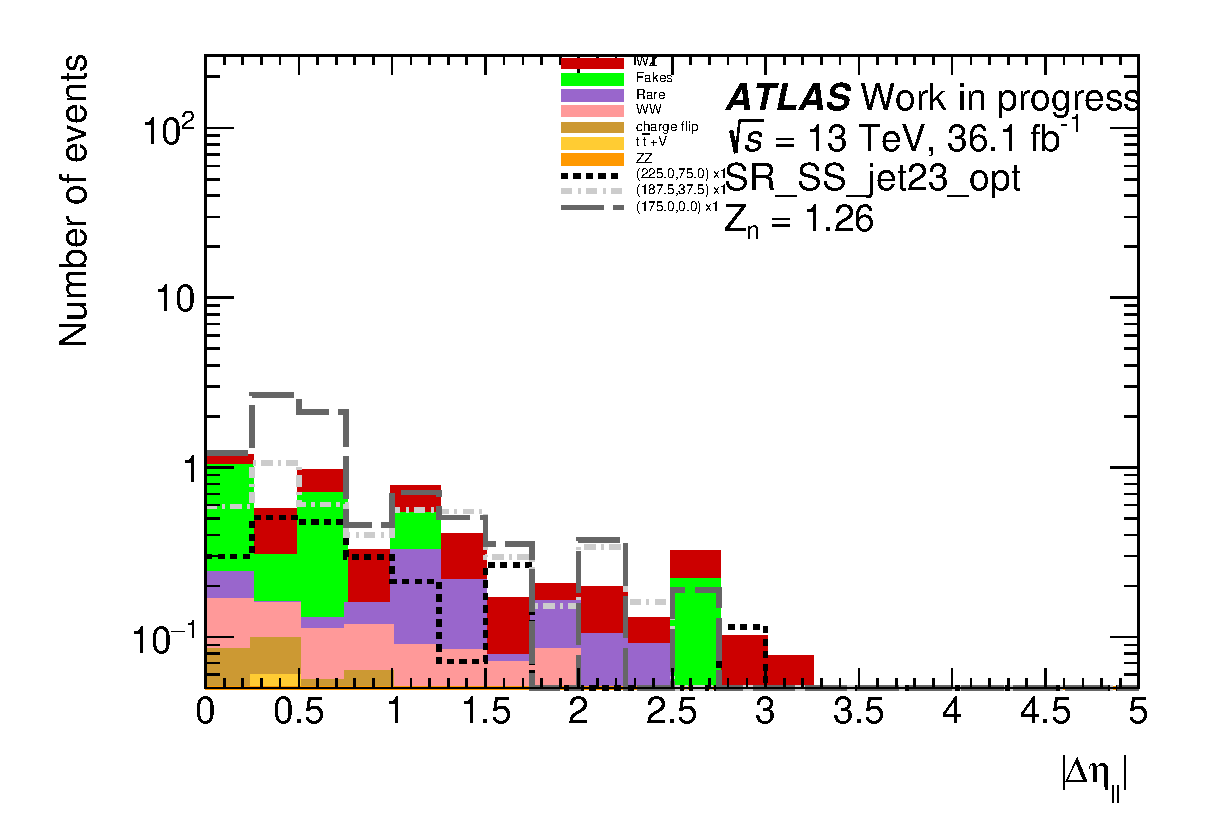
\includegraphics[width=0.45\linewidth]{data/plot/plot_SR/dEta_SR_SS_jet23_opt_0}
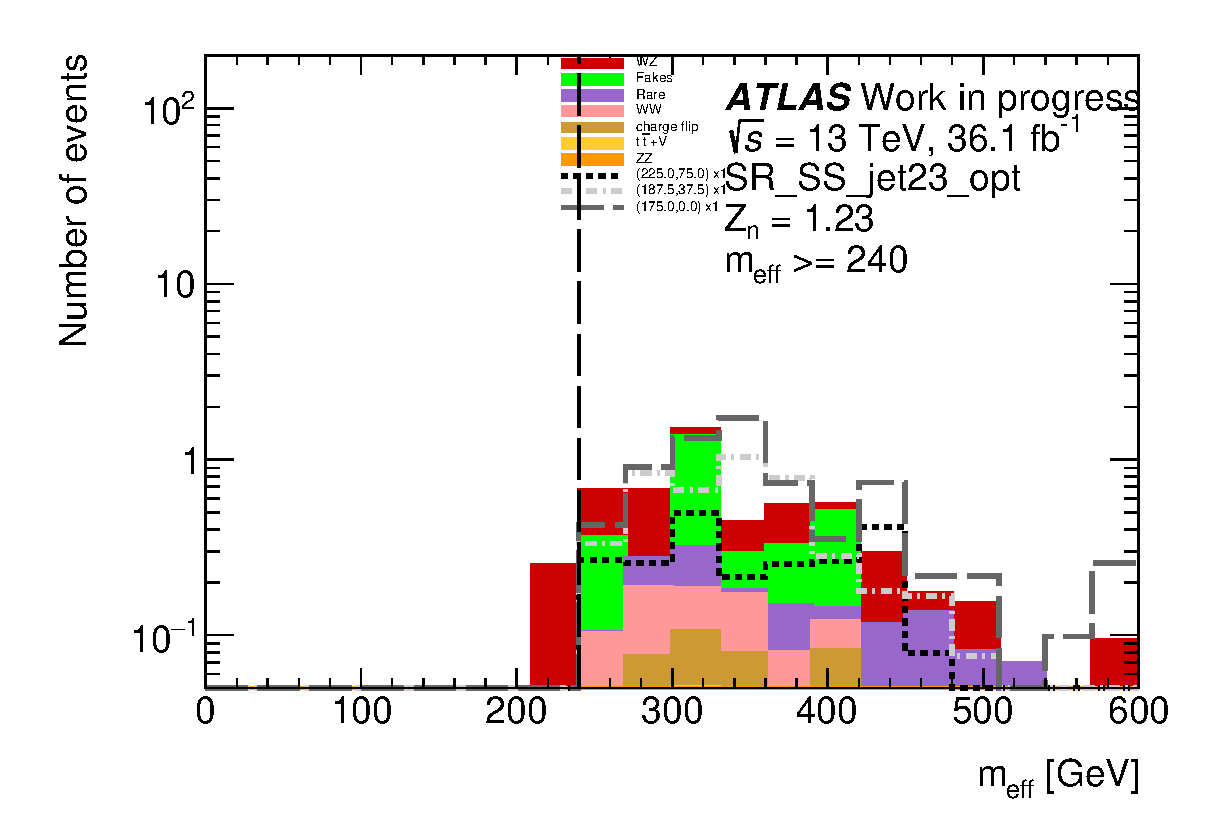
\includegraphics[width=0.45\linewidth]{data/plot/plot_SR/meff_SR_SS_jet23_opt_0}\\
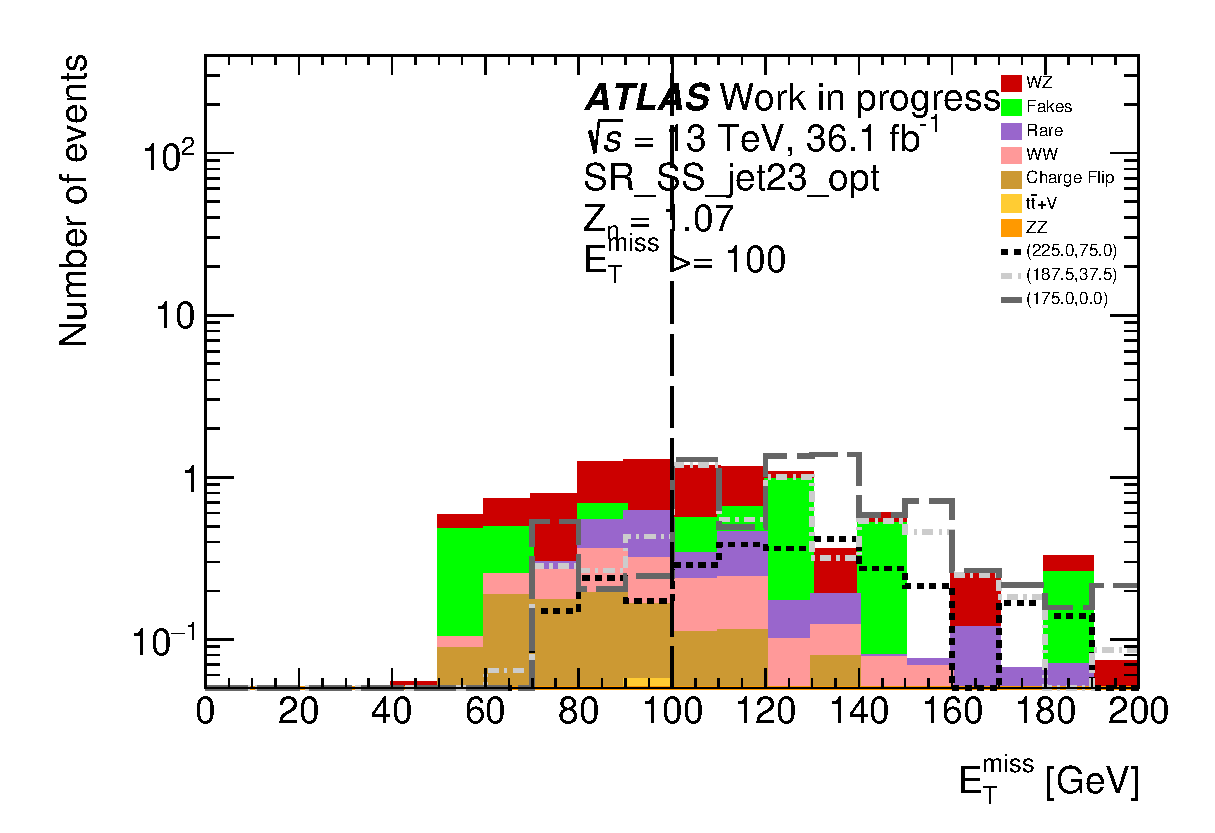
\includegraphics[width=0.45\linewidth]{data/plot/plot_SR/MET_SR_SS_jet23_opt_0}
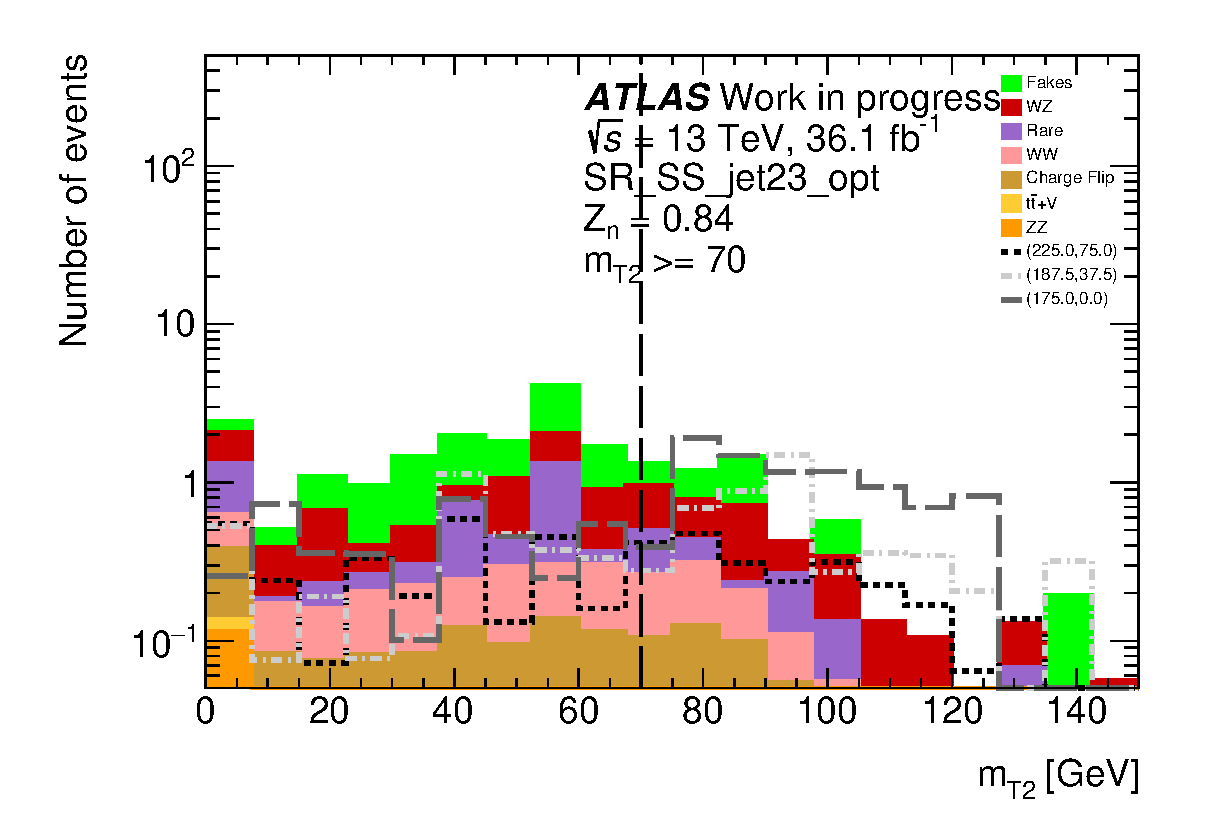
\includegraphics[width=0.45\linewidth]{data/plot/plot_SR/mTtwo_SR_SS_jet23_opt_0}\\
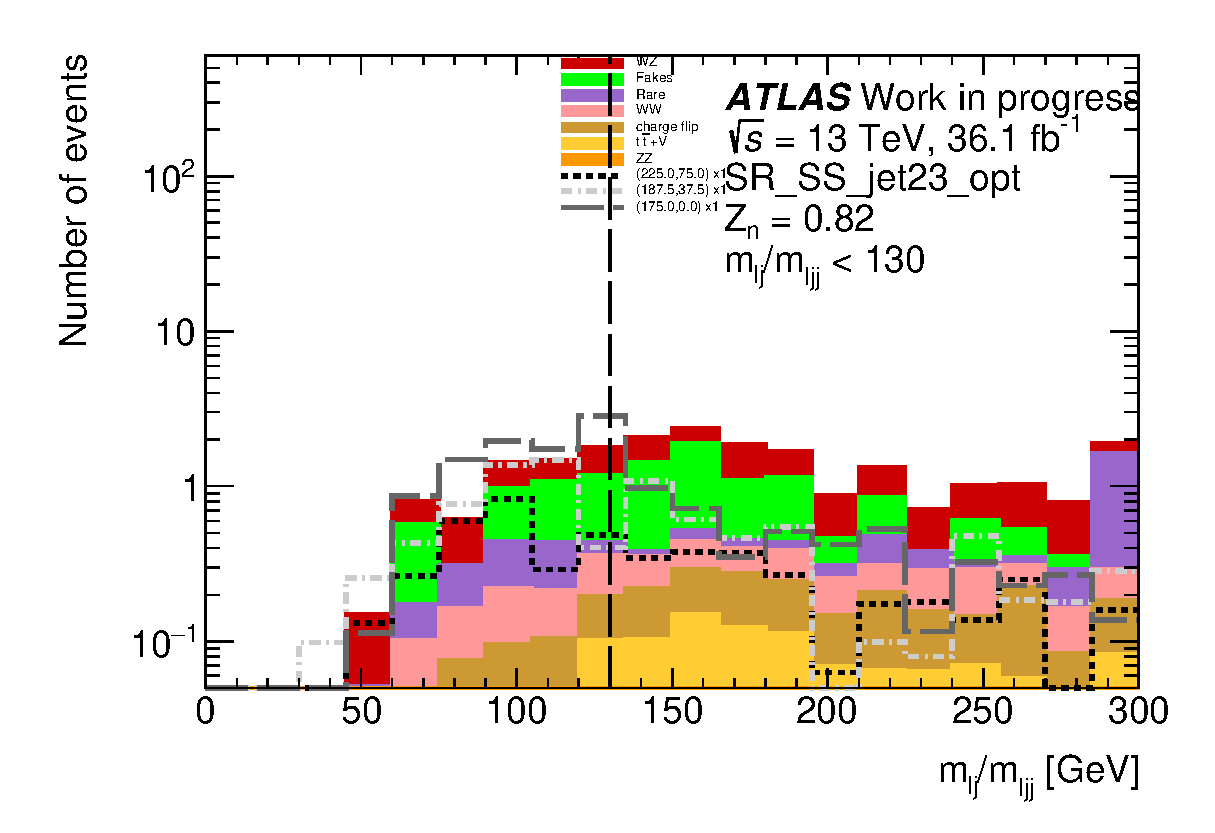
\includegraphics[width=0.45\linewidth]{data/plot/plot_SR/mlj_SR_SS_jet23_opt_0}
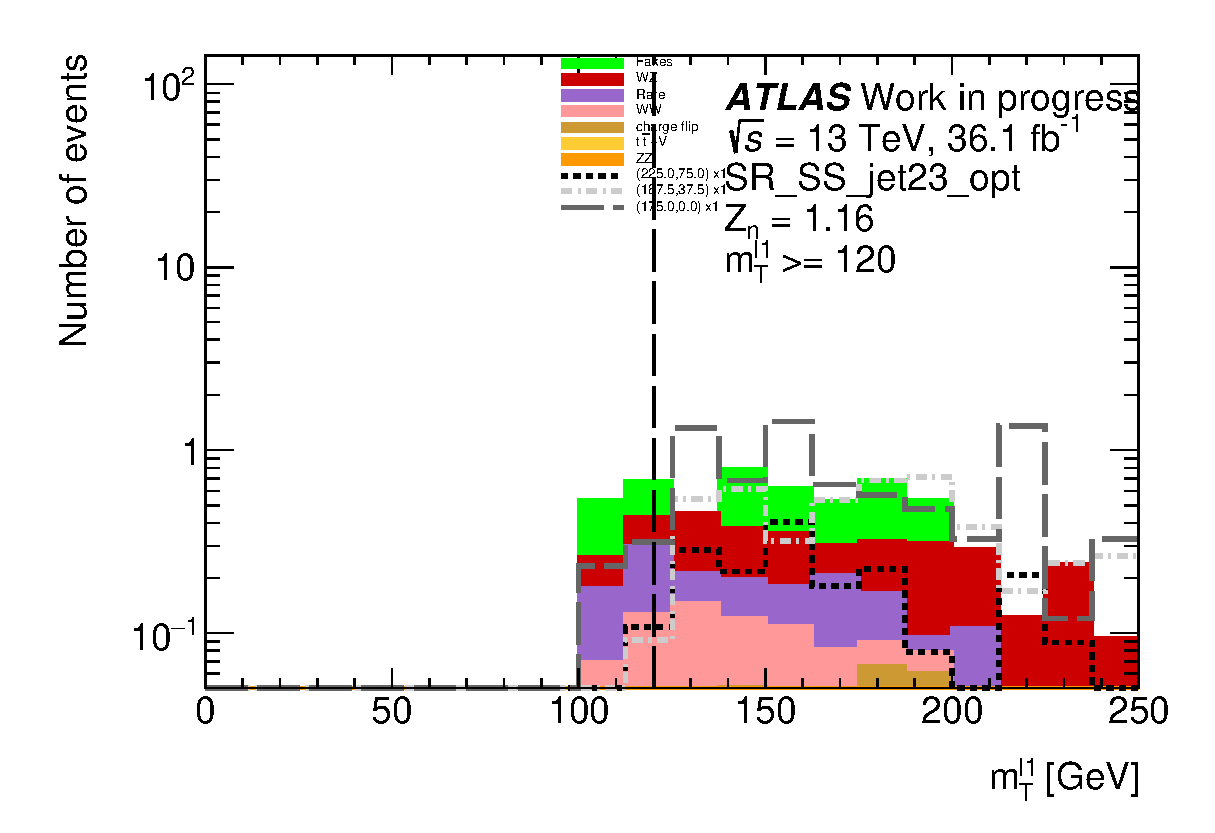
\includegraphics[width=0.45\linewidth]{data/plot/plot_SR/mt1_SR_SS_jet23_opt_0}\\
\caption{The N-1 plots for SRjet23.}
\label{fig:SRjet23_N1}
\end{figure}

The expected combined signal significances for different mass points are shown in figure \ref{fig:SR_expected_limit}.
A flat 25 \% systematic uncertainty are included.
The combined signal significances are calculated by adding the signal significances of the two signal regions in quadrature.
The figure shows considerable signal significances, in particular for the compressed region, where $m_{\tilde{\chi}_1^\pm , \tilde{\chi}_2^0} - m_{\tilde{\chi}_1^0}$ are close to the mass of Higgs boson ($\sim 125$ GeV).

\begin{figure}[htpb]
\centering
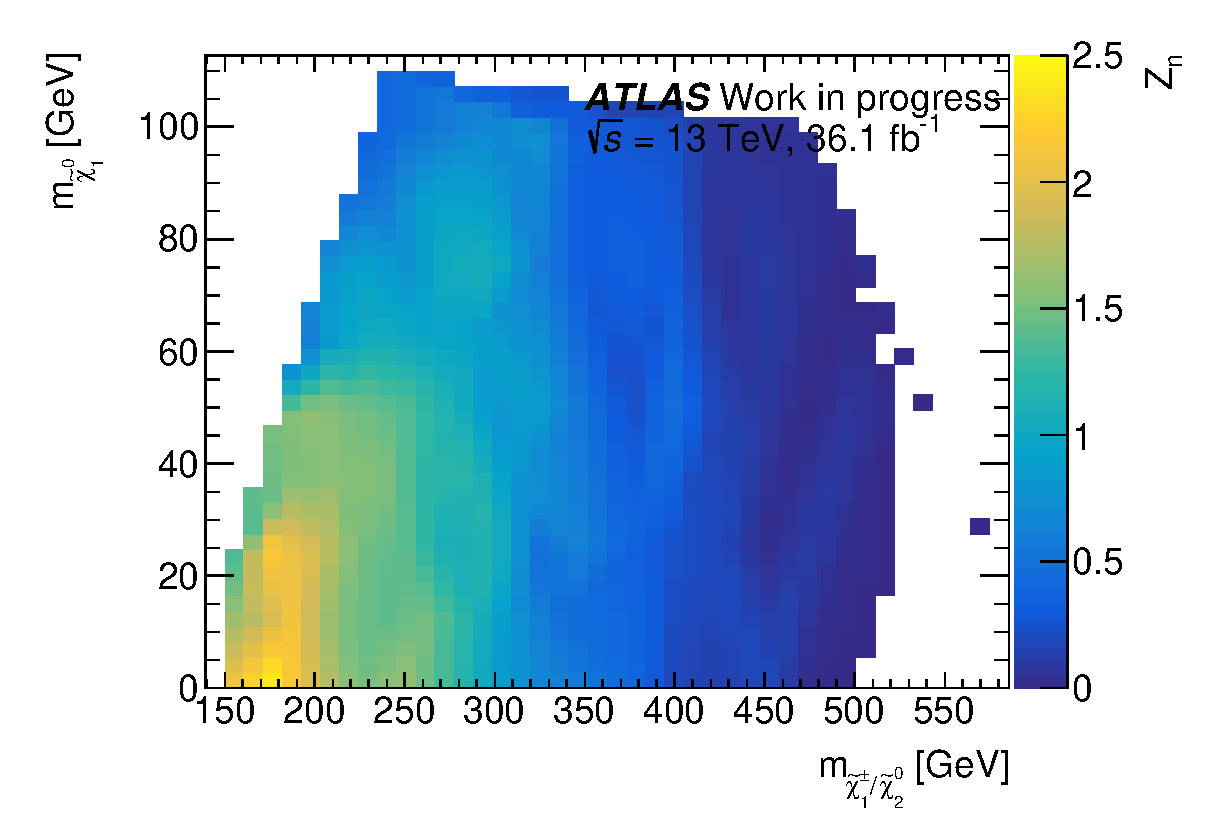
\includegraphics[width=0.5\linewidth]{data/plot/plot_SR/combine_significance_0}
\caption{The expected combined signal significances for different mass points.}
\label{fig:SR_expected_limit}
\end{figure}

%************************************************
\chapter{Background estimation}
\label{ch:BG}
%************************************************

The charge flip background and the fake lepton background are the two dominant backgrounds that their original particles in the final state come from the SM, but not the SUSY signal. Because of the mis-reconstruction, they pass the selections of the SRs. This type of background will be estimated by using the data-driven method.

\section{Charge flip background}
\subsection{Sources for charge flip background}
The charge flip background is due to the mis-identification of the sign of the charge of a lepton, after the reconstruction.
The sign of the charge is determined by the direction of the curvature of the track.
There are two main sources for the mis-identification for the direction of the curvature.

The first source is described by the figure \ref{fig:charge_flip_bremsstrahlung}.
It is the case that the lepton interacts with the material of the detector, and a photon is emitted by the process of bremsstrahlung.
The emitted photon further produces a pair of electron and positron, namely the $\gamma$ conversion.
As shown in figure \ref{fig:charge_flip_bremsstrahlung}, if the most of the energy is carried by the positron $e^{+}$ (the purple track), the direction of the curvature of the reconstructed track (the orange track) will be reversed.
Thus, the charge of the lepton is flipped.
Because the amount of this mis-identification depends on the number of hits with the detector, and hence depends on $|\eta|$ of the original track.

\begin{figure}
\centering
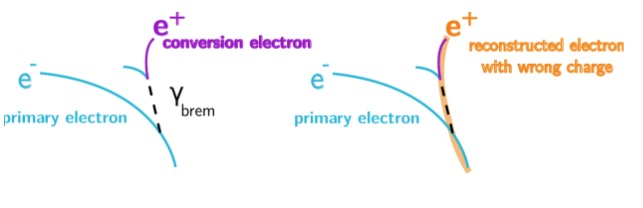
\includegraphics[width=\textwidth]{data/photo/charge_flip/Brem.jpg}
\caption{This shows how the track of the electron is incorrectly reconstructed (the orange track), due to the process of bremsstrahlung and $\gamma$ conversion.}
\label{fig:charge_flip_bremsstrahlung}
\end{figure}

The second source is described by the figure \ref{fig:charge_flip_high_pt}.
When the $p_T$ of the lepton is very high, the track of the lepton will be almost a straight line.
The curvature of the track will be close to zero, and the sign of the curvature will be difficult to distinguish.
As a result, the sign of the charge of the lepton will be incorrectly assigned.
The chance to have this problem obviously depends on $p_T$ of the lepton.

\begin{figure}
\centering
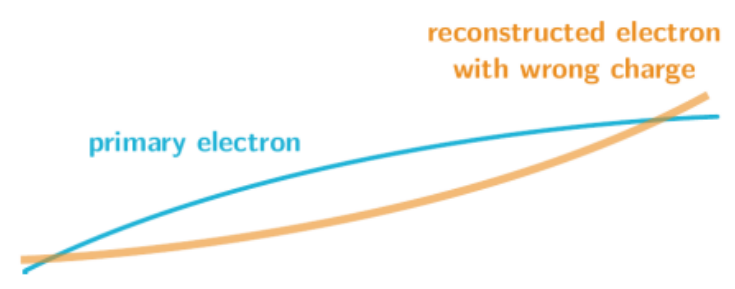
\includegraphics[width=\textwidth]{data/photo/charge_flip/WrongTrack.png}
\caption{This shows how the track of the electron is incorrectly reconstructed (the orange track), due to very high $p_T$ of the electron.}
\label{fig:charge_flip_high_pt}
\end{figure}

Compared to an electron, the charge of a reconstructed muon will be less often to be mis-identified.
The first reason is that a muon is heavier than an electron.
This will reduce the chance of the process of bremsstrahlung.
The second reason is that muons can reach to the muon spectrometer, which is the outer part of the detector, while most electrons cannot.
This means that the length of the track of a muon, which can be detected by the tracker, is longer than that of an electron.
Hence, the reconstructed curvature of the track for muons can be more accurate, and it reduces the chance of the mis-identification due to the high $p_T$.
Because most of the charge flip background comes from electrons, we only estimate the charge flip background for electrons.

\subsection{Likelihood method}
\label{sec:likelihood_method}
The probability that the charge of an electron is mis-identified is denoted by the charge-flip rate $\epsilon_i$, where the index i represents the dependency on the $p_T$ and $\eta$ of the electron.
The value of index i is found by splitting the variables $p_T$ and $|\eta|$ into different 2-dimensional bins, and the binning for the $p_T$ and $|\eta|$ is described by the table \ref{tab:binning_charge_flip}. The index i of $\epsilon_i$ is defined by the index of the bin.

\begin{table}[htbp]
\centering
\begin{tabular}{|c|c|}
\hline
Variable & Boundary of the bins \\
\hline
$p_T$ (GeV) &  25, 60, 90, 130, 150, 1000 \\
\hline
$|\eta|$ & 0, 0.50, 1.00, 1.37, 1.52, 1.80, 2.00, 2.47 \\
\hline
\end{tabular}
\caption{Binning in $p_T$ and $|\eta|$ for the charge-flip rate $\epsilon_i$.}
\label{tab:binning_charge_flip}
\end{table}

Suppose that, before the reconstruction, there are $m^{ij}_{OS}$ opposite-sign events with the leading lepton in bin $i$ and the sub-leading lepton in bin $j$, and similarly there are $m^{ij}_{SS}$ same-sign events.
After the reconstruction, due to the charge flip, there are $M^{ij}_{OS}$ opposite-sign events and $M^{ij}_{SS}$ same-sign events.
The number of events after the reconstruction is given by
\begin{equation}
M^{ij}_{OS} = (1-\epsilon_i) (1-\epsilon_j) m^{ij}_{OS} + \epsilon_i (1-\epsilon_j) m^{ij}_{SS} + (1-\epsilon_i) \epsilon_j m^{ij}_{SS} + \epsilon_i \epsilon_j m^{ij}_{OS}
\end{equation}
\begin{equation}
M^{ij}_{SS} = (1-\epsilon_i) (1-\epsilon_j) m^{ij}_{SS} + \epsilon_i (1-\epsilon_j) m^{ij}_{OS} + (1-\epsilon_i) \epsilon_j m^{ij}_{OS} + \epsilon_i \epsilon_j m^{ij}_{SS}
\label{equ:MSS}
\end{equation}
From equation \ref{equ:MSS}, the number of reconstructed same-sign events due to the real opposite-sign events, i.e. the charge flip BG , denoted by $N^{ij}_{SS}$, is
\begin{equation}
N^{ij}_{SS} = \epsilon_i (1-\epsilon_j) m^{ij}_{OS} + (1-\epsilon_i) \epsilon_j m^{ij}_{OS}
\label{equ:NSS}
\end{equation}
In the SRs, $m^{ij}_{OS}$ is the number of OS events before the reconstruction, but finally pass all selections in SRs.
$M^{ij}_{OS}$ is the total number of events that pass all selections in SRs, but replace SS requirement by OS.
Because $m^{ij}_{OS}$ is much larger than $m^{ij}_{SS}$ and the measured charge-flip rate $\epsilon_i$ is about $10^{-3}$, $m^{ij}_{OS}$ can be estimated by
\begin{align}
M^{ij}_{OS} &\approx (1-\epsilon_i) (1-\epsilon_j) m^{ij}_{OS} \\
m^{ij}_{OS} &\approx \frac{ M^{ij}_{OS} }{ (1-\epsilon_i) (1-\epsilon_j) }
\label{equ:mapp1} \\
m^{ij}_{OS} &\approx M^{ij}_{OS} \\
m^{ij}_{OS} &\approx M^{ij}_{OS} + M^{ij}_{SS}
\label{equ:mapp2}
\end{align}
By substituting equation \ref{equ:mapp2} into \ref{equ:NSS}, the charge flip BG can be estimated by $M^{ij}_{OS}$, $M^{ij}_{SS}$ and the charge-flip rate $\epsilon_i$,
\begin{align}
N^{ij}_{SS} &= \epsilon_i (1-\epsilon_j) m^{ij}_{OS} + (1-\epsilon_i) \epsilon_j m^{ij}_{OS} \\
&= [ \epsilon_i (1-\epsilon_j) + (1-\epsilon_i) \epsilon_j ] m^{ij}_{OS} \label{equ:NSS3}\\
&\approx p_{ij} (M^{ij}_{OS} + M^{ij}_{SS}) \\
&=p_{ij} N^{ij}
\label{equ:NSS2}
\end{align}
where $p_{ij}$ and $N^{ij}$ are
\begin{align}
\begin{split}
p_{ij} &= \epsilon_i (1-\epsilon_j) + (1-\epsilon_i) \epsilon_j \\
N^{ij} &= M^{ij}_{OS} + M^{ij}_{SS}
\end{split}
\end{align}
The probability density function of $N^{ij}_{SS}$, with the given values of $N^{ij}$ and $\epsilon_i$, can be described by the Poisson distribution with the mean value $\lambda = p_{ij} N^{ij}$.
\begin{align}
P(N^{ij}_{SS}|N^{ij},\epsilon_i,\epsilon_j) &= \frac{ \lambda^{N^{ij}_{SS}} e^{-\lambda} }{N^{ij}_{SS}!} \\
 &= \frac{ (p_{ij} N^{ij})^{N^{ij}_{SS}} e^{- p_{ij} N^{ij}} }{N^{ij}_{SS}!}
\label{equ:poisson}
\end{align}

In order to estimate the charge flip BG, we need to measure the charge-flip rate $\epsilon_i$.
The charge-flip rate is measured as a function of $p_T$ and $|\eta|$ by using a likelihood method, based on the 2015 and 2016 data.
A control region is used to select $Z \rightarrow ee$ processes.
Inside the control region, exactly 2 signal electrons are required.
Also, a Z mass window of 80 GeV $<m_{ll}<$100 GeV is used.
In this control region, the total number of events $N^{ij}$ and the SS events $N^{ij}_{SS}$ in each bin can be measured.
By using the equation \ref{equ:poisson}, the charge-flip rate $\epsilon_i$ can be measured by using the following likelihood method.

The likelihood function $L$ is defined by
\begin{align}
L(\epsilon_i,\epsilon_j|N^{ij},N^{ij}_{SS}) &= \prod_{ij} P(N^{ij}_{SS}|N^{ij},\epsilon_i,\epsilon_j) \\
&= \prod_{ij} \frac{ (p_{ij} N^{ij})^{N^{ij}_{SS}} e^{- p_{ij} N^{ij}} }{N^{ij}_{SS}!} \\
\end{align}
Given the measured values of $N^{ij}$ and $N^{ij}_{SS}$ in each bin, by maximizing the likelihood function over all possible values of $\epsilon_i$, the value of $\epsilon_i$ can be estimated.
By taking the negative logarithm, it is equivalent to minimize $- \ln L$.
\begin{align}
- \ln L
&= - \ln \prod_{ij} \frac{ (p_{ij} N^{ij})^{N^{ij}_{SS}} e^{- p_{ij} N^{ij}} }{N^{ij}_{SS}!} \\
&= - \sum_{ij} \ln \frac{ (p_{ij} N^{ij})^{N^{ij}_{SS}} e^{- p_{ij} N^{ij}} }{N^{ij}_{SS}!} \\
&= - \sum_{ij} \Big[ N^{ij}_{SS} \ln (p_{ij} N^{ij}) - p_{ij} N^{ij} - \ln( N^{ij}_{SS}!) \Big] \\
&= - \sum_{ij} \Big[ N^{ij}_{SS} \ln (p_{ij} N^{ij}) - p_{ij} N^{ij} \Big] + \text{constant} \\
&= - \sum_{ij} \Big[ N^{ij}_{SS} \ln (N^{ij}[\epsilon_i (1-\epsilon_j) + (1-\epsilon_i) \epsilon_j]) - N^{ij}[\epsilon_i (1-\epsilon_j) + (1-\epsilon_i) \epsilon_j] \Big] + \text{constant}
\end{align}

\subsection{Background subtraction}
\label{sec:Background_subtraction}
By minimizing $- \ln L$ described in the previous section, the value of the charge-flip rate $\epsilon_i$ can be measured by using the data in the control region.
In order to have better input values of $N^{ij}$ and $N^{ij}_{SS}$, the number of events should mainly come from $Z \rightarrow ee$ processes, and other processes should be subtracted.
The number of events from other processes can be estimated by the sideband region: 60 GeV $<m_{ll}<$ 80 GeV and 100 GeV $<m_{ll}<$ 120 GeV.
The corrected values of $N^{ij}$ and $N^{ij}_{SS}$ are given by
\begin{align}
N_{80,100;\text{corrected}} = N_{80,100} - 20 \Big( \frac{N_{60,80} + N_{80,100}}{20 + 20} \Big)
\end{align}
In the sideband subtraction, the number of events in the sideband region should be normalized to the width of the central region.
In general, given the number of events in the central region $N_{\text{central}}$, the left sideband region $N_{\text{left}}$ and the right sideband region $N_{\text{right}}$, and their corresponding width $w_{\text{central}}$, $w_{\text{left}}$ and $w_{\text{right}}$, the corrected values $N_{\text{central,corrected}}$ are given by
\begin{align}
N_{\text{central,corrected}} = N_{\text{central}} - w_{\text{central}} \Big( \frac{N_{\text{left}} + N_{\text{right}}}{w_{\text{left}} + w_{\text{right}}} \Big)
\end{align}

\subsection{Results without systematic uncertainty}
\label{sec:results_stat}
Figure \ref{fig:charge_flip_data_stat} shows the measured values of the charge-flip rate $\epsilon_i$ by using the data.
The errors only include the uncertainties in the likelihood method due to the statistics, denoted by $\epsilon_{\text{lik,data}}$.

\begin{figure}
\centering
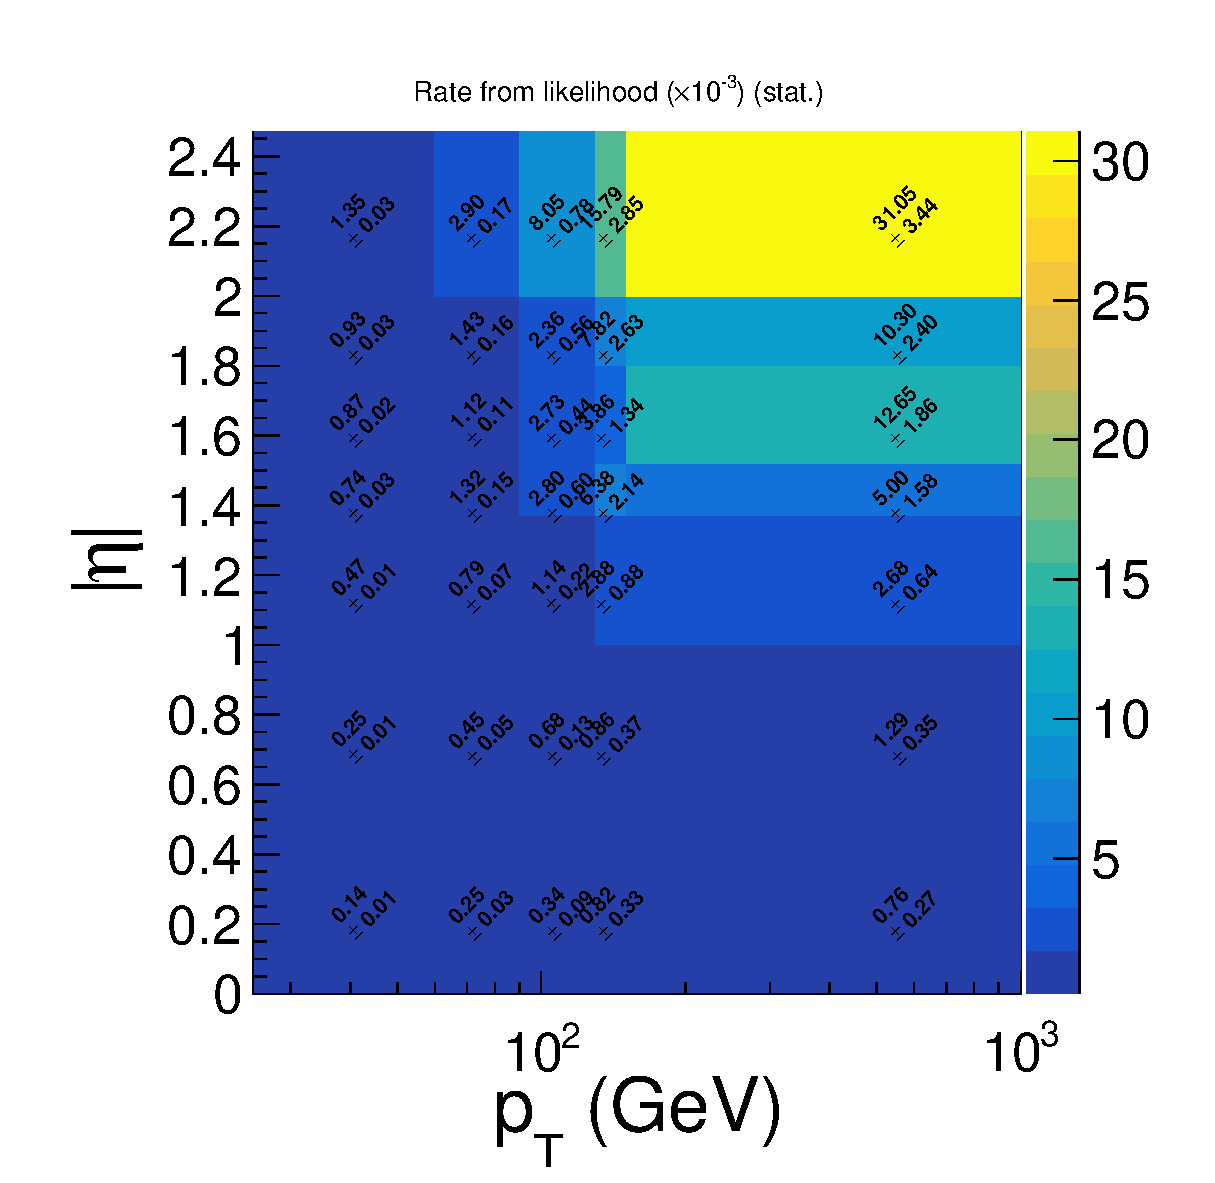
\includegraphics[width=\textwidth]{data/plot/charge_flip/FitPlots/data_cf_rate_stat.eps}
\caption{The measured values of the charge-flip rate $\epsilon_i$ in data. Only uncertainties due to the likelihood method are included.}
\label{fig:charge_flip_data_stat}
\end{figure}

\subsection{Systematic uncertainties due to background subtraction}
\label{sec:sys_background_subtraction}
The systematic uncertainties due to background subtraction is estimated by the variations of different central widths and sideband widths.
The following are the nominal central region and sideband region, and their 4 variations. \\
The nominal background subtraction:
\begin{itemize}
\item Central region: 80 - 100 GeV; Sideband width: 20 GeV
\end{itemize}
The 4 variations for background subtraction:
\begin{itemize}
\item Central region: 80 - 100 GeV; Sideband width: 15 GeV
\item Central region: 80 - 100 GeV; Sideband width: 25 GeV
\item Central region: 75 - 105 GeV; Sideband width: 20 GeV
\item Central region: 80 - 100 GeV; no background subtraction
\end{itemize}

For each bin, the largest deviation from the nominal among these variations is the systematic uncertainty due to background subtraction.
\begin{equation}
\sigma_{\text{bgk}} = \max \{| \sigma_{\text{nominal}} - \sigma_{\text{variation}} |\}
\end{equation}

Figure \ref{fig:charge_flip_sys_background_subtraction} shows the variations of the resulting charge flip rate, due to these 4 variations.
\begin{figure}
\centering
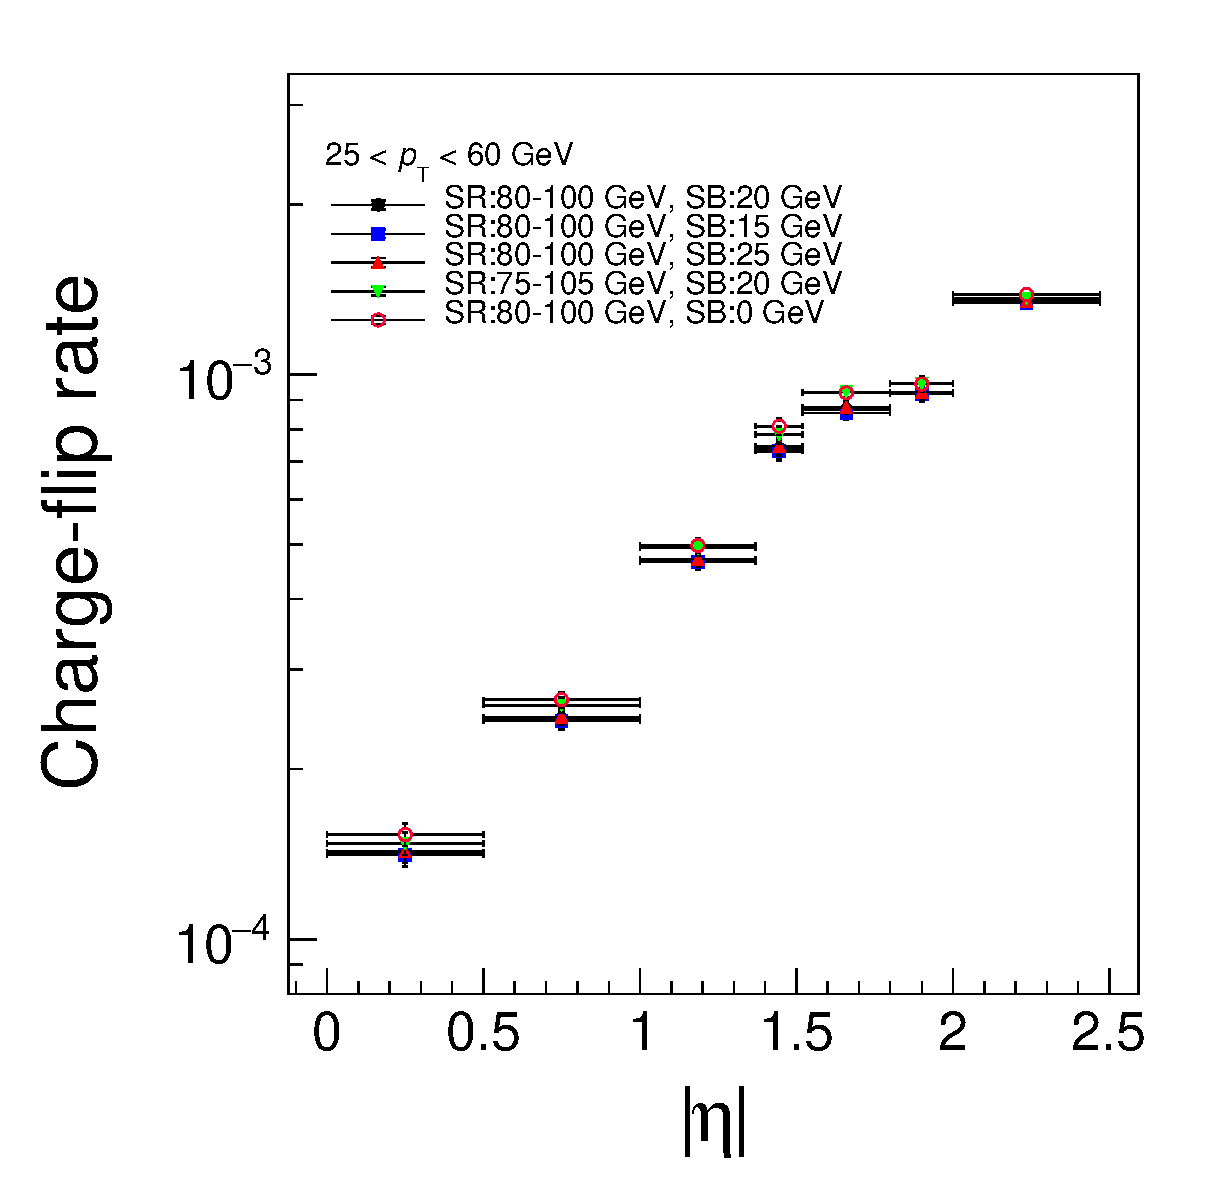
\includegraphics[width=0.3\textwidth]{data/plot/charge_flip/FitPlots/data_cf_comparison_0.eps}
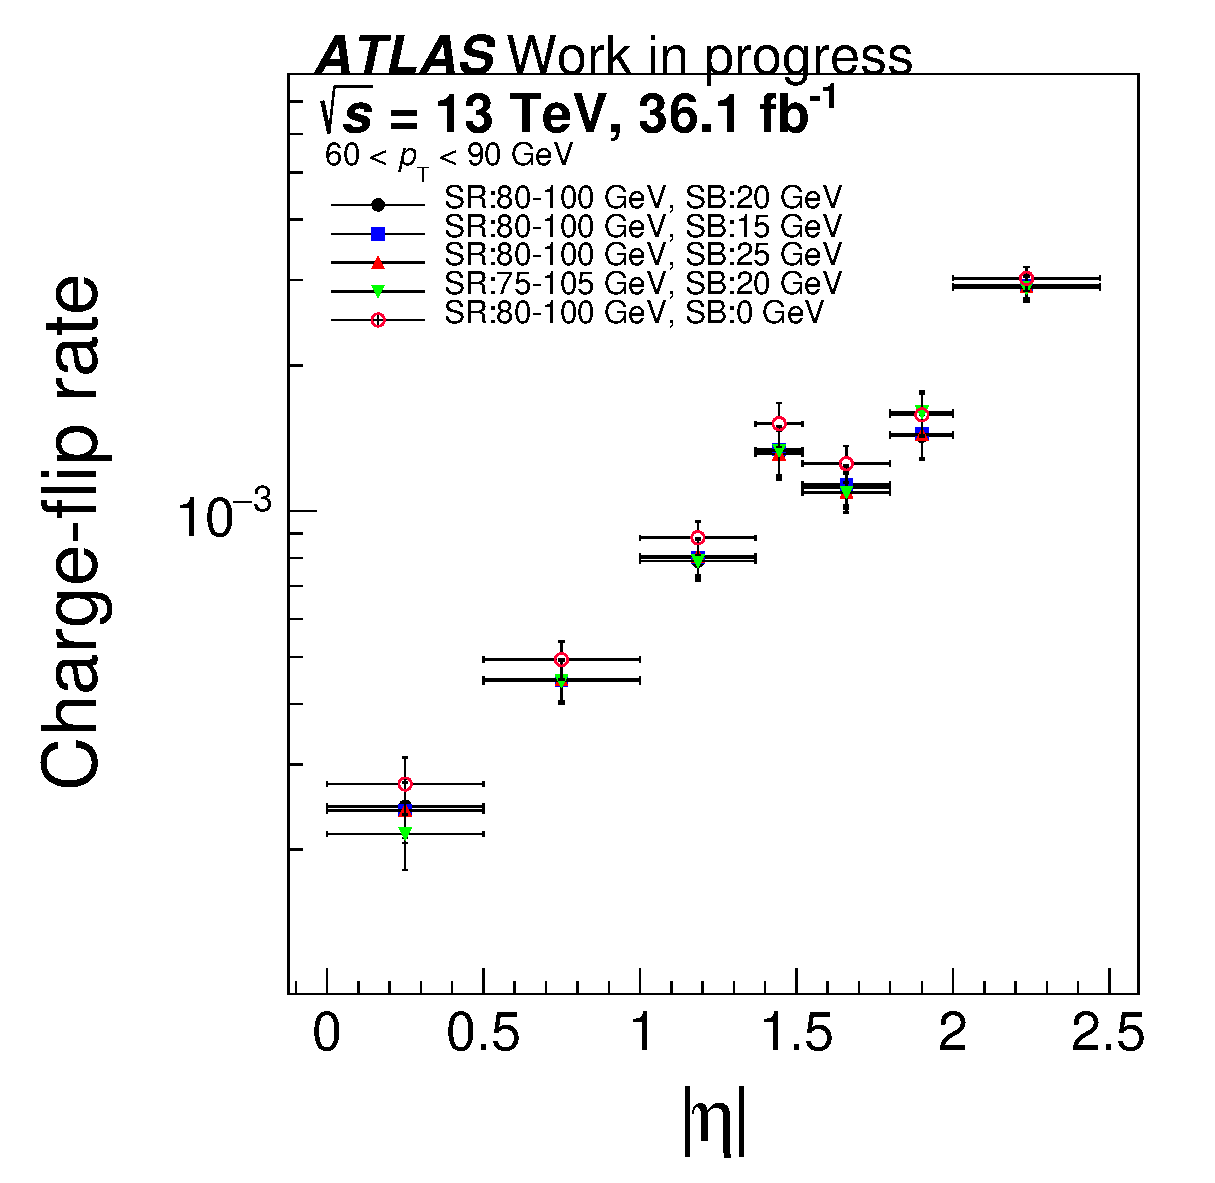
\includegraphics[width=0.3\textwidth]{data/plot/charge_flip/FitPlots/data_cf_comparison_1.eps}
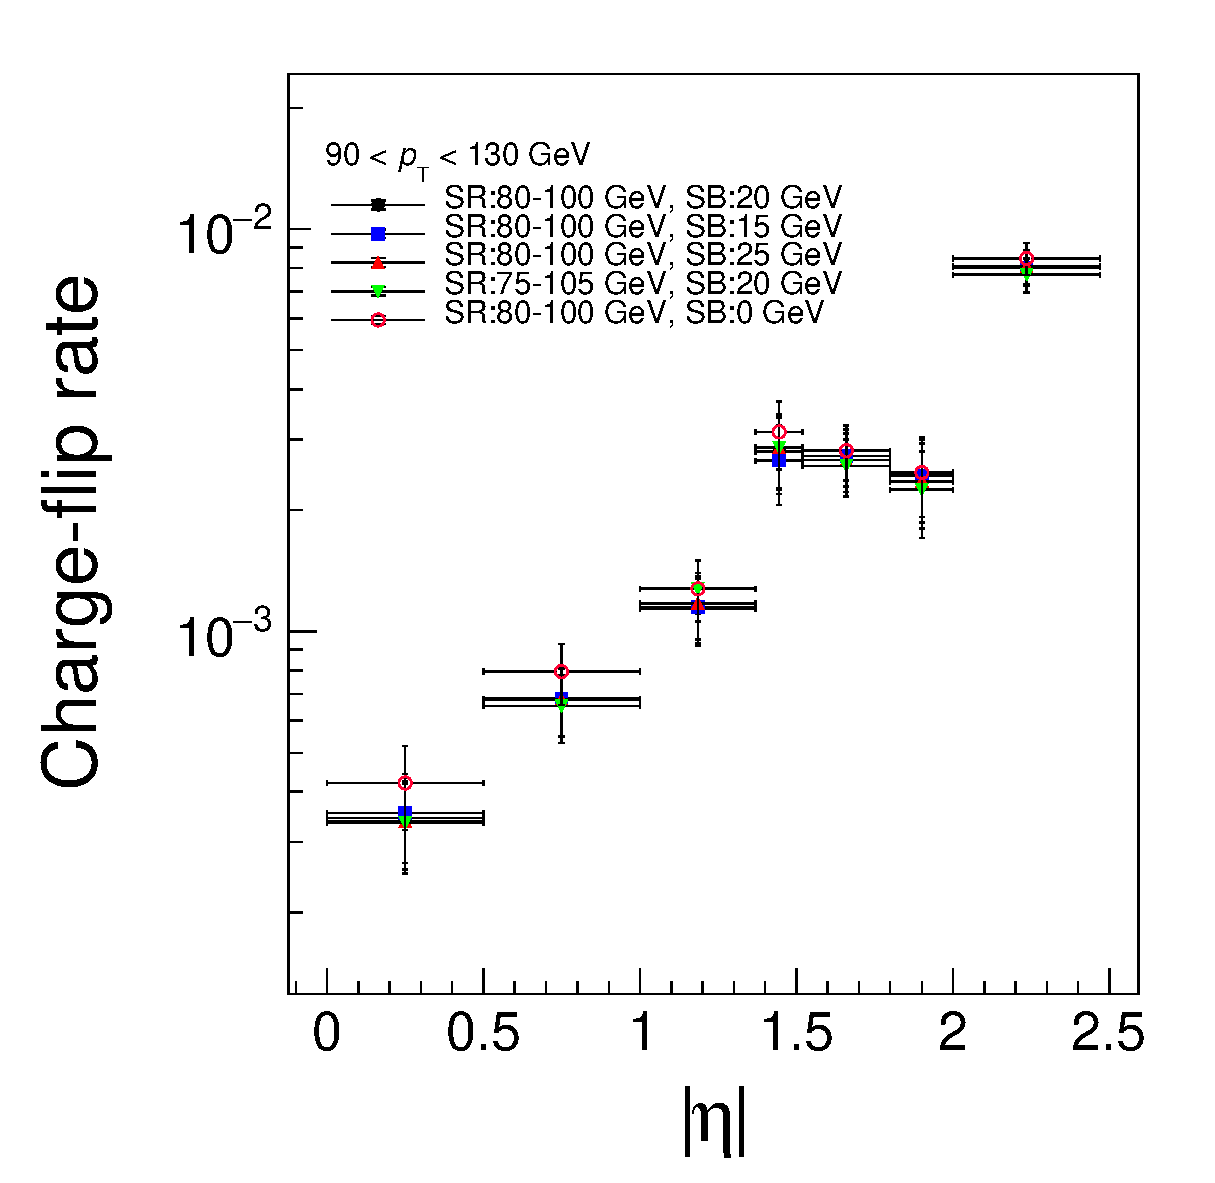
\includegraphics[width=0.3\textwidth]{data/plot/charge_flip/FitPlots/data_cf_comparison_2.eps} \\
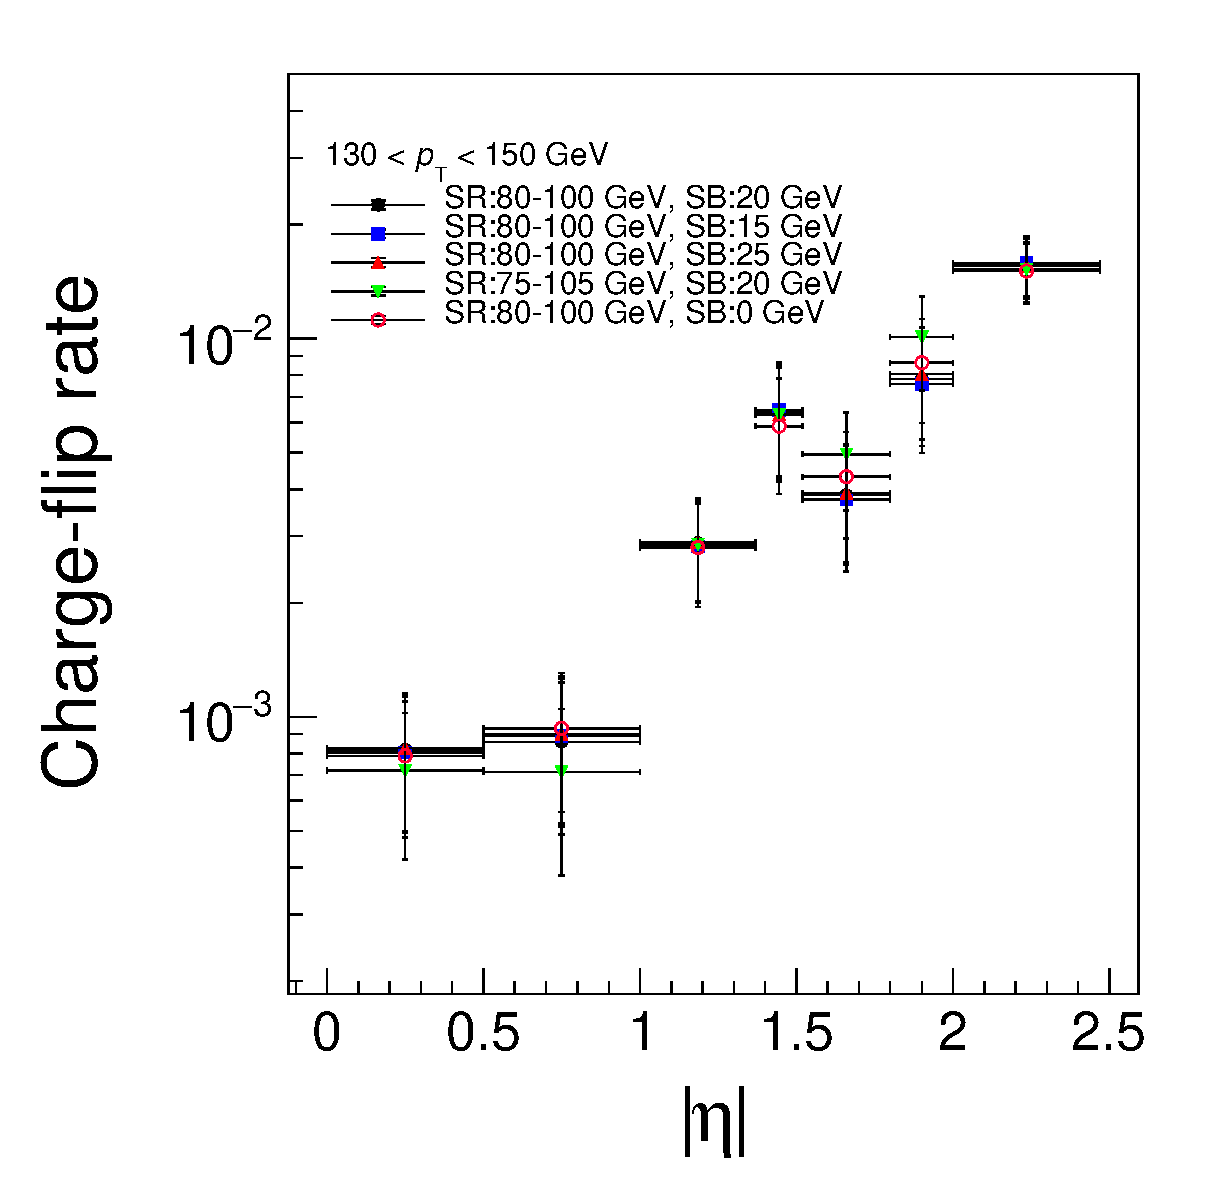
\includegraphics[width=0.3\textwidth]{data/plot/charge_flip/FitPlots/data_cf_comparison_3.eps}
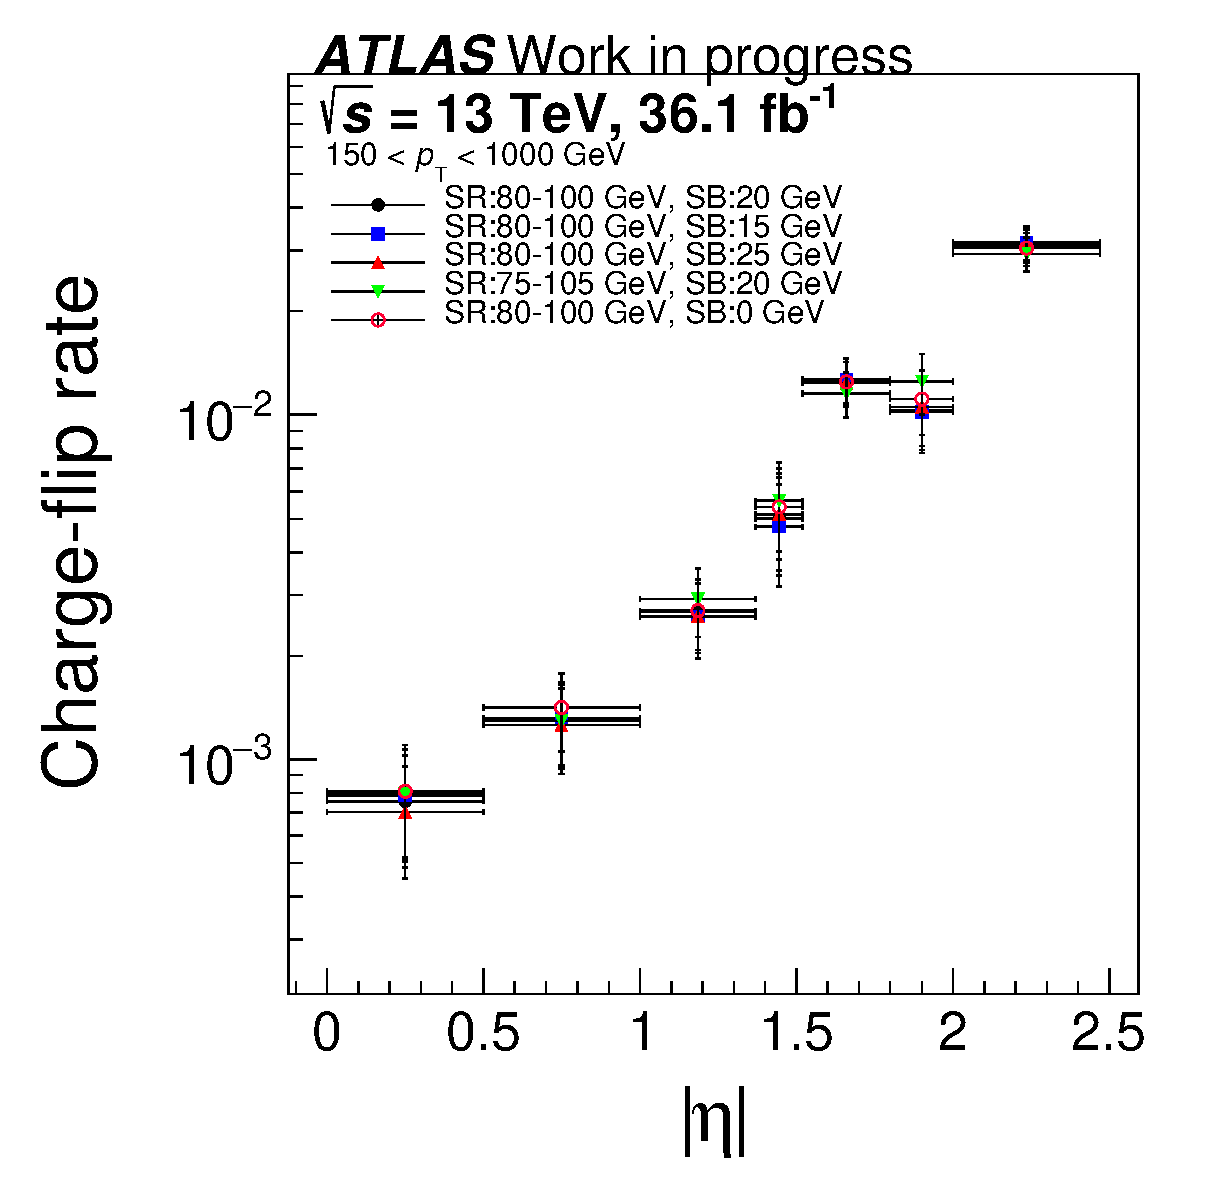
\includegraphics[width=0.3\textwidth]{data/plot/charge_flip/FitPlots/data_cf_comparison_4.eps}
\caption{The systematic variations of the charge-flip rate $\epsilon_i$ in data, due to the background subtraction.}
\label{fig:charge_flip_sys_background_subtraction}
\end{figure}

\subsection{Systematic uncertainties due to likelihood method}
\label{sec:sys_likelihood}
The systematic uncertainties due to likelihood method are estimated by the difference between the likelihood method and the MC truth method.
In the MC truth method, the charge-flip rate is estimated by using the truth information in $Z \rightarrow ee$ MC samples inside the control region.
The control region requires exactly 2 signal electrons.
The following are the procedures to match the reconstructed electron to the original electron, and hence the original electric charge can be found.
Figure \ref{fig:charge_flip_MC_match} shows how the original electron is found in the decay process described in figure \ref{fig:charge_flip_bremsstrahlung}. In this procedure, some reconstructed electrons will be ignored.
\begin{figure}
\centering
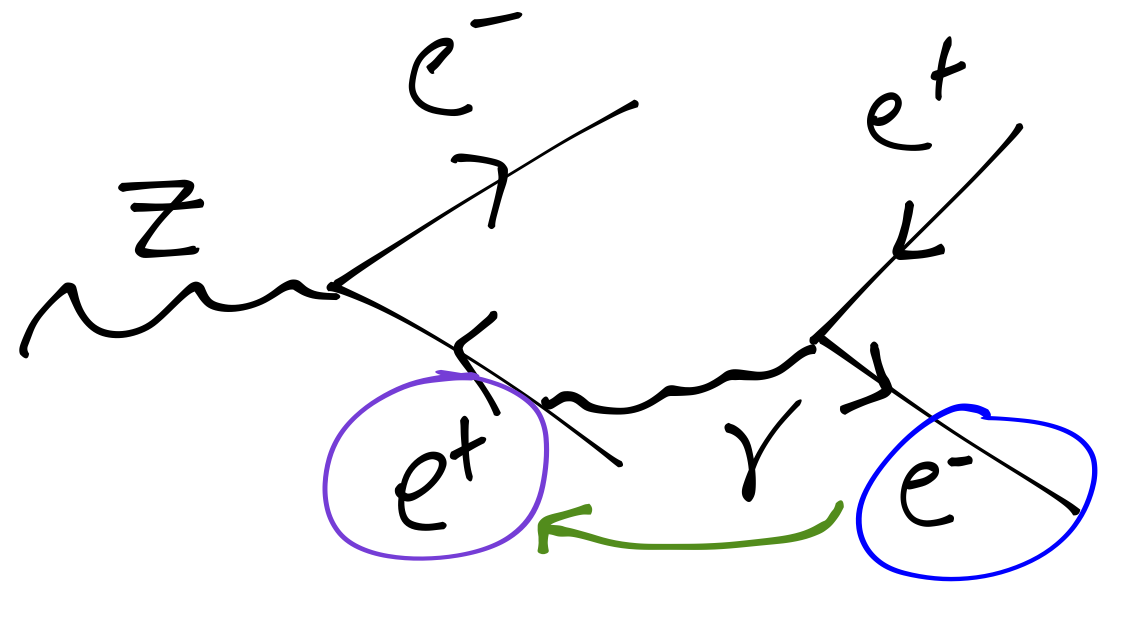
\includegraphics[width=0.5\textwidth]{data/photo/charge_flip/MC-truth.png}
\caption{This diagram shows how the original electron is found through the decay chain.}
\label{fig:charge_flip_MC_match}
\end{figure}
\begin{enumerate}
\item The reconstructed electron will be matched to the truth particle with the smallest $\Delta R$ within the cone $\Delta R < 0.1$. If no any truth particles can be found inside the cone, the reconstructed electron will be ignored.
\item If the truth particle is not an electron, it will be ignored.
\item If the origin of the truth electron is not a Z boson, it will be ignored.
\item If the daughter particle of the Z boson is not an electron, it will be ignored.
\item The charge of the daughter electron from the Z boson is the original charge of the reconstructed electron.
\end{enumerate}

Only the events with two reconstructed electrons that are not ignored in the above procedure are considered.
$N_{\text{total}}$ is the total number of electrons in these events, and $N_{\text{flipped}}$ is the number of electrons that the original charge and the reconstructed charge are different.
By calculating the ratio in each bin, the charge flip rate can be estimated by using the MC truth information.
\begin{equation}
\epsilon_{\text{MC truth}} = \frac{N_{\text{flipped}}}{N_{\text{total}}}
\end{equation}

The systematic uncertainties due to likelihood method $\sigma_{\text{truth}}$ is then given by \\
for MC,
\begin{equation}
\sigma_{\text{truth,MC}} = | \epsilon_{\text{lik,MC}} - \epsilon_{\text{MC truth}} |
\end{equation}
for data,
\begin{equation}
\sigma_{\text{truth,data}} = \epsilon_{\text{lik,data}} \times \frac{\sigma_{\text{truth,MC}}}{\epsilon_{\text{lik,MC}}}
\end{equation}

Figure \ref{fig:charge_flip_sys_truth} shows the comparison of the resulting charge flip rate, between the likelihood method and the MC truth method, by using the $Z \rightarrow ee$ MC samples.
\begin{figure}
\centering
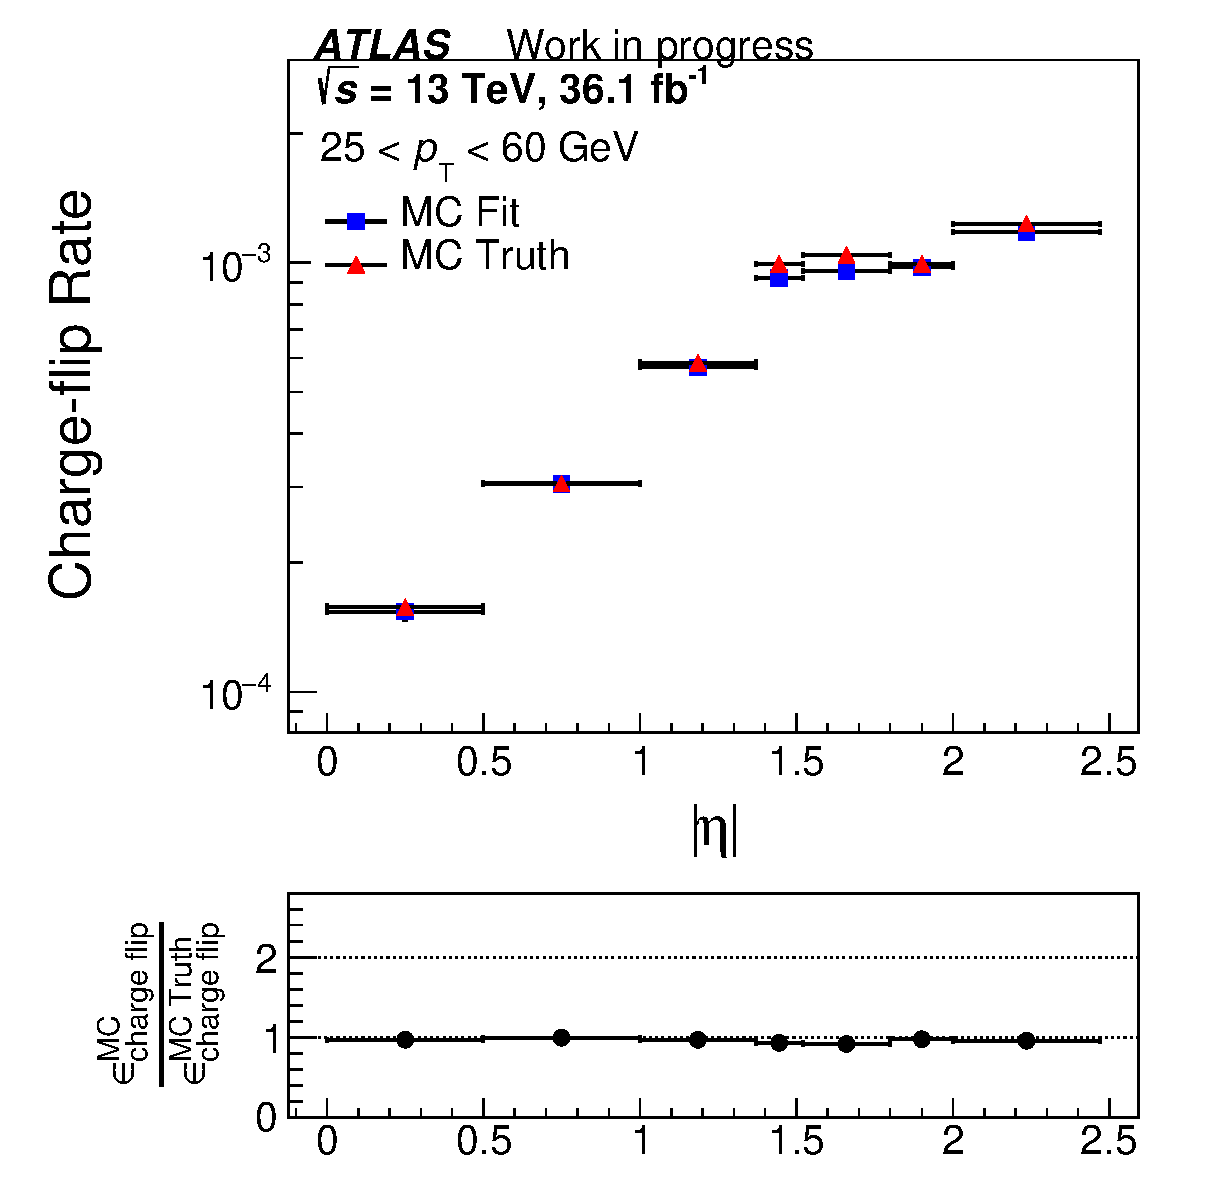
\includegraphics[width=0.3\textwidth]{data/plot/charge_flip/FitPlots/mc_cf_rate_0.eps}
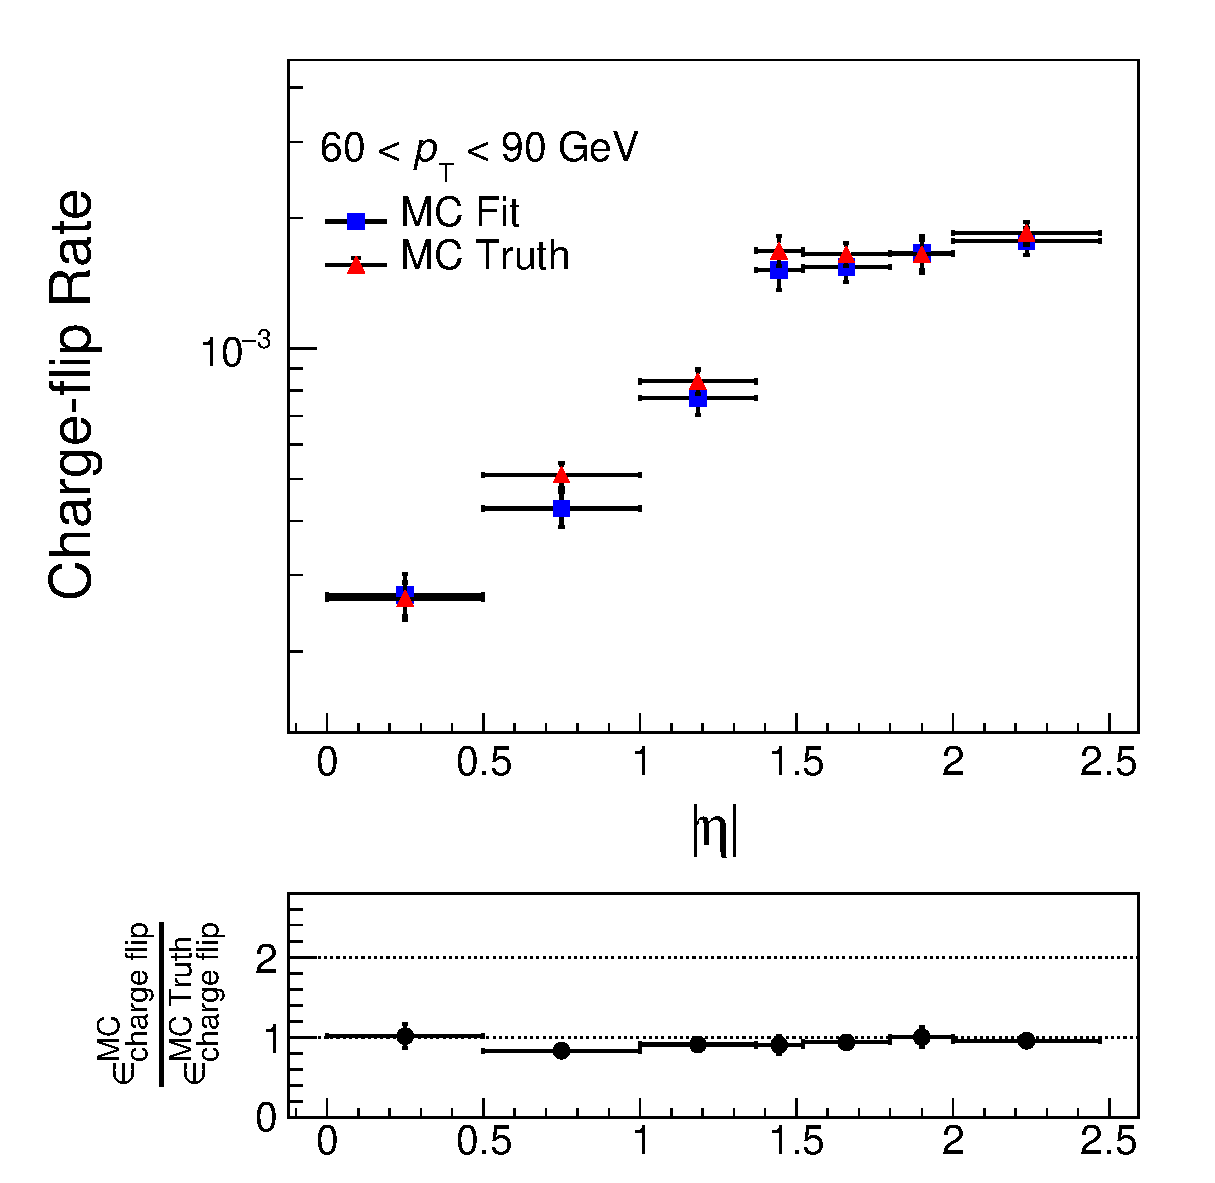
\includegraphics[width=0.3\textwidth]{data/plot/charge_flip/FitPlots/mc_cf_rate_1.eps}
\includegraphics[width=0.3\textwidth]{data/plot/charge_flip/FitPlots/mc_cf_rate_2.eps} \\
\includegraphics[width=0.3\textwidth]{data/plot/charge_flip/FitPlots/mc_cf_rate_3.eps}
\includegraphics[width=0.3\textwidth]{data/plot/charge_flip/FitPlots/mc_cf_rate_4.eps}
\caption{The comparison between the likelihood method and the MC truth method, by using the $Z \rightarrow ee$ MC samples. Hence, the systematic uncertainties due to likelihood method can be estimated.}
\label{fig:charge_flip_sys_truth}
\end{figure}

\subsection{Results with total uncertainties}
\label{sec:charge_flip_results_stat}
The total systematic uncertainties is the quadratic sum of systematic uncertainties due to the background subtraction and the likelihood method, described in section \ref{sec:sys_background_subtraction} and \ref{sec:sys_likelihood} respectively.
\begin{equation}
\sigma_{\text{sys}} = \sqrt{\sigma_{\text{bgk}} ^2+ \sigma_{\text{truth}} ^2}
\end{equation}
The total uncertainties is the quadratic sum of the total systematic uncertainties and the statistical uncertainties in the likelihood method.
\begin{equation}
\sigma_{\text{tot}} = \sqrt{\sigma_{\text{sys}} ^2 + \sigma_{\text{lik}} ^2}
\label{equ:tot_error}
\end{equation}

Figure \ref{fig:charge_flip_data_tot} shows the measured values of the charge-flip rate $\epsilon_i$ by using the data, with total uncertainties described in equation \ref{equ:tot_error}.

\begin{figure}
\centering
\includegraphics[width=\textwidth]{data/plot/charge_flip/FitPlots/data_cf_rate_tot.eps}
\caption{The measured values of the charge-flip rate $\epsilon_i$ in data, with total uncertainties.}
\label{fig:charge_flip_data_tot}
\end{figure}

\subsection{MC validation}
\label{sec:charge_flip_MC_validation}
The charge flip rate can be validated by using the $Z \rightarrow ee$ MC samples.
By using the equation \ref{equ:mapp1} and \ref{equ:NSS3}, $N^{ij}_{SS}$ can be approximated by
\begin{align}
N^{ij}_{SS} &= [ \epsilon_i (1-\epsilon_j) + (1-\epsilon_i) \epsilon_j ] m^{ij}_{OS} \\
&\approx [ \epsilon_i (1-\epsilon_j) + (1-\epsilon_i) \epsilon_j ] \frac{ M^{ij}_{OS} }{ (1-\epsilon_i) (1-\epsilon_j) } \\
&= \frac{\epsilon_i (1-\epsilon_j) + (1-\epsilon_i) \epsilon_j}{(1-\epsilon_i) (1-\epsilon_j)} M^{ij}_{OS}
\end{align}
Also, in the equation \ref{equ:MSS}, $m^{ij}_{SS}$ is zero for the $Z \rightarrow ee$ MC samples, we have
\begin{align}
M^{ij}_{SS} &= \epsilon_i (1-\epsilon_j) m^{ij}_{OS} + (1-\epsilon_i) \epsilon_j m^{ij}_{OS} \\
&= N^{ij}_{SS}
\end{align}
Hence, it is expected that
\begin{align}
M^{ij}_{SS} \approx \frac{\epsilon_i (1-\epsilon_j) + (1-\epsilon_i) \epsilon_j}{(1-\epsilon_i) (1-\epsilon_j)} M^{ij}_{OS}
\end{align}
By weighting the OS events in MC with the weight,
\begin{align}
\text{weight} = \frac{\epsilon_i (1-\epsilon_j) + (1-\epsilon_i) \epsilon_j}{(1-\epsilon_i) (1-\epsilon_j)}
\end{align}
the weighted OS events and the SS events will be close to each other.
This can be used to validate the charge flip rate.
Figure shows the comparison between the weighted OS events and the SS events, with different variables.
All event weights are applied, except the charge flip scale factor.
The weighted OS events and the SS events agree within the uncertainties.
\begin{figure}
\centering
\includegraphics[width=0.3\textwidth]{data/plot/charge_flip/ReweightPlots/plots_NOchfSF/mc_pt_1.pdf}
\includegraphics[width=0.3\textwidth]{data/plot/charge_flip/ReweightPlots/plots_NOchfSF/mc_pt_2.pdf} \\
\includegraphics[width=0.3\textwidth]{data/plot/charge_flip/ReweightPlots/plots_NOchfSF/mc_eta_1.pdf}
\includegraphics[width=0.3\textwidth]{data/plot/charge_flip/ReweightPlots/plots_NOchfSF/mc_eta_2.pdf} \\
\includegraphics[width=0.3\textwidth]{data/plot/charge_flip/ReweightPlots/plots_NOchfSF/mc_mll.pdf}
\includegraphics[width=0.3\textwidth]{data/plot/charge_flip/ReweightPlots/plots_NOchfSF/mc_phi_1.pdf}
\includegraphics[width=0.3\textwidth]{data/plot/charge_flip/ReweightPlots/plots_NOchfSF/mc_phi_2.pdf}
\caption{The comparison between the weighted OS events and the SS events, with different variables.}
\end{figure}

\section{Fake lepton background}
\label{sec:fake_background}
\subsection{Sources for fake lepton background}
The fake lepton background is ascribed to the case that other particle like meson, hadron and photon is mis-identified as a lepton, after the reconstruction.
Three types of fake lepton background are described as follows.
\begin{itemize}
\item Heavy-flavor fakes:
\begin{itemize}
\item It comes from semi-leptonic decays of heavy-quark (b or c) hadrons in jets
\end{itemize}
\item Light-flavor fakes:
\begin{itemize}
\item It comes from semi-leptonic decays of light-quark hadrons in jets
\item or is due to mis-reconstructions of jets with light-quark hadrons
\end{itemize}
\item photon conversion:
\begin{itemize}
\item It comes from the pair production from a photon
\end{itemize}
\end{itemize}
These leptons do not often pass the lepton identification cuts and have large impact parameters.
They are also not well-isolated.

\subsection{Matrix method}
The fake lepton background is estimated by the matrix method.
The input of this method is the real and fake efficiencies of electron and muon, in different bins of $p_T$ and $|\eta|$, which is measured in the following sections.
This method will estimate the amount of fake lepton background, by counting the number of loose and tight leptons in data.
The tight leptons in our analysis are the signal leptons, and the loose leptons are baseline leptons but not signal leptons.

The probability that a real electron (or muon) passes the signal selection (i.e. tight lepton) is denoted by the real efficiency $\epsilon$.
The probability that a real electron (or muon) does not pass the signal selection (i.e. loose lepton) is denoted by $\bar{\epsilon} = 1 - \epsilon$.
Similarly, the probability that a fake electron (or muon) passes the signal selection (i.e. tight lepton) is denoted by the fake efficiency $f$.
The probability that a fake electron (or muon) does not pass the signal selection (i.e. loose lepton) is denoted by $\bar{f} = 1 - f$.
Although there is no subscripts and superscripts for the efficiencies $e$ and $f$, these efficiencies are different for different flavours of the leptons (electron or muon), and also in different $p_T$-$|\eta|$ bins.

For simplicity, we first consider the case with only one leptons. We will then generalize to the case with two leptons.
By the definition of the efficiencies, the relation between the number of real/fake leptons and the number of tight/loose leptons is given by the following matrix.
\begin{equation}
\left( \begin{array}{c}
N_T \\
N_L
\end{array} \right)
=
\left( \begin{array}{cc}
\epsilon & f \\
\bar{\epsilon} & \bar{f}
\end{array} \right)
\left( \begin{array}{c}
N_R \\
N_F
\end{array} \right)
\label{equ:fake_eff_def}
\end{equation}
Because the number of tight/loose leptons can be counted in data, $\left( \begin{array}{c}
N_T \\
N_L
\end{array} \right)$ is known.
By inverting the matrix, the original number of fake leptons can be calculated.
\begin{align}
\begin{split}
\left( \begin{array}{c}
0 \\
N_F
\end{array} \right)
&=
\left( \begin{array}{cc}
0 & 0 \\
0 & 1
\end{array} \right)
\left( \begin{array}{c}
N_R \\
N_F
\end{array} \right) \\
&=
\left( \begin{array}{cc}
0 & 0 \\
0 & 1
\end{array} \right)
\left( \begin{array}{cc}
\epsilon & f \\
\bar{\epsilon} & \bar{f}
\end{array} \right)^{-1}
\left( \begin{array}{c}
N_T \\
N_L
\end{array} \right)
\end{split}
\end{align}
The fake lepton background, which is the number of tight lepton due to the fake lepton, $N_T'$, can then be found, by re-apply the matrix in equation \ref{equ:fake_eff_def}.
\begin{align}
\begin{split}
\left( \begin{array}{c}
N_T' \\
N_L'
\end{array} \right)
&=
\left( \begin{array}{cc}
\epsilon & f \\
\bar{\epsilon} & \bar{f}
\end{array} \right)
\left( \begin{array}{c}
0 \\
N_F
\end{array} \right) \\
&=
\left( \begin{array}{cc}
\epsilon & f \\
\bar{\epsilon} & \bar{f}
\end{array} \right)
\left( \begin{array}{cc}
0 & 0 \\
0 & 1
\end{array} \right)
\left( \begin{array}{cc}
\epsilon & f \\
\bar{\epsilon} & \bar{f}
\end{array} \right)^{-1}
\left( \begin{array}{c}
N_T \\
N_L
\end{array} \right) \\
N_T'
&=
\left( \begin{array}{cc}
\epsilon & f \\
\end{array} \right)
\left( \begin{array}{cc}
0 & 0 \\
0 & 1
\end{array} \right)
\left( \begin{array}{cc}
\epsilon & f \\
\bar{\epsilon} & \bar{f}
\end{array} \right)^{-1}
\left( \begin{array}{c}
N_T \\
N_L
\end{array} \right) \\
\end{split}
\end{align}

To generalize to the case with two leptons, equation \ref{equ:fake_eff_def} becomes
\begin{equation}
\left( \begin{array}{c}
N_{TT} \\
N_{TL} \\
N_{LT} \\
N_{LL}
\end{array} \right)
=
\left( \begin{array}{cccc}
\epsilon_1 \epsilon_2 & \epsilon_1 f_2 & f_1 \epsilon_2 & f_1 f_2 \\
\epsilon_1 \bar{\epsilon_2} & \epsilon_1 \bar{f_2} & f_1 \bar{\epsilon_2} & f_1 \bar{f_2} \\
\bar{\epsilon_1} \epsilon_2 & \bar{\epsilon_1} f_2 & \bar{f_1} \epsilon_2 & \bar{f_1} f_2 \\
\bar{\epsilon_1} \bar{\epsilon_2} & \bar{\epsilon_1} \bar{f_2} & \bar{f_1} \bar{\epsilon_2} & \bar{f_1} \bar{f_2}
\end{array} \right)
\left( \begin{array}{c}
N_{RR} \\
N_{RF} \\
N_{FR} \\
N_{FF}
\end{array} \right)
\end{equation}
where the subscripts 1 and 2 of the efficiencies denote the leading lepton and sub-leading lepton respectively.
The two letters in the subscript of $N$ describe the types of the leading and sub-leading lepton respectively.
$N_{RF}$, $N_{FR}$, $N_{FF}$ can be found by inverting the matrix.
\begin{align}
\begin{split}
\left( \begin{array}{c}
0 \\
N_{RF} \\
N_{FR} \\
N_{FF}
\end{array} \right)
&=
\left( \begin{array}{cccc}
0 & 0 & 0 & 0 \\
0 & 1 & 0 & 0 \\
0 & 0 & 1 & 0 \\
0 & 0 & 0 & 1
\end{array} \right)
\left( \begin{array}{c}
N_{RR} \\
N_{RF} \\
N_{FR} \\
N_{FF}
\end{array} \right) \\
&=
\left( \begin{array}{cccc}
0 & 0 & 0 & 0 \\
0 & 1 & 0 & 0 \\
0 & 0 & 1 & 0 \\
0 & 0 & 0 & 1
\end{array} \right)
\left( \begin{array}{cccc}
\epsilon_1 \epsilon_2 & \epsilon_1 f_2 & f_1 \epsilon_2 & f_1 f_2 \\
\epsilon_1 \bar{\epsilon_2} & \epsilon_1 \bar{f_2} & f_1 \bar{\epsilon_2} & f_1 \bar{f_2} \\
\bar{\epsilon_1} \epsilon_2 & \bar{\epsilon_1} f_2 & \bar{f_1} \epsilon_2 & \bar{f_1} f_2 \\
\bar{\epsilon_1} \bar{\epsilon_2} & \bar{\epsilon_1} \bar{f_2} & \bar{f_1} \bar{\epsilon_2} & \bar{f_1} \bar{f_2}
\end{array} \right)^{-1}
\left( \begin{array}{c}
N_{TT} \\
N_{TL} \\
N_{LT} \\
N_{LL}
\end{array} \right)
\end{split}
\end{align}
The fake lepton background, which is the number of tight-tight lepton due to the fake lepton, $N_{TT}'$, can then be found.
\begin{align}
\begin{split}
\left( \begin{array}{c}
N_{TT}' \\
N_{TL}' \\
N_{LT}' \\
N_{LL}'
\end{array} \right)
&=
\left( \begin{array}{cccc}
\epsilon_1 \epsilon_2 & \epsilon_1 f_2 & f_1 \epsilon_2 & f_1 f_2 \\
\epsilon_1 \bar{\epsilon_2} & \epsilon_1 \bar{f_2} & f_1 \bar{\epsilon_2} & f_1 \bar{f_2} \\
\bar{\epsilon_1} \epsilon_2 & \bar{\epsilon_1} f_2 & \bar{f_1} \epsilon_2 & \bar{f_1} f_2 \\
\bar{\epsilon_1} \bar{\epsilon_2} & \bar{\epsilon_1} \bar{f_2} & \bar{f_1} \bar{\epsilon_2} & \bar{f_1} \bar{f_2}
\end{array} \right)
\left( \begin{array}{c}
0 \\
N_{RF} \\
N_{FR} \\
N_{FF}
\end{array} \right) \\
&=
\left( \begin{array}{cccc}
\epsilon_1 \epsilon_2 & \epsilon_1 f_2 & f_1 \epsilon_2 & f_1 f_2 \\
\epsilon_1 \bar{\epsilon_2} & \epsilon_1 \bar{f_2} & f_1 \bar{\epsilon_2} & f_1 \bar{f_2} \\
\bar{\epsilon_1} \epsilon_2 & \bar{\epsilon_1} f_2 & \bar{f_1} \epsilon_2 & \bar{f_1} f_2 \\
\bar{\epsilon_1} \bar{\epsilon_2} & \bar{\epsilon_1} \bar{f_2} & \bar{f_1} \bar{\epsilon_2} & \bar{f_1} \bar{f_2}
\end{array} \right)
\left( \begin{array}{cccc}
0 & 0 & 0 & 0 \\
0 & 1 & 0 & 0 \\
0 & 0 & 1 & 0 \\
0 & 0 & 0 & 1
\end{array} \right)
\left( \begin{array}{cccc}
\epsilon_1 \epsilon_2 & \epsilon_1 f_2 & f_1 \epsilon_2 & f_1 f_2 \\
\epsilon_1 \bar{\epsilon_2} & \epsilon_1 \bar{f_2} & f_1 \bar{\epsilon_2} & f_1 \bar{f_2} \\
\bar{\epsilon_1} \epsilon_2 & \bar{\epsilon_1} f_2 & \bar{f_1} \epsilon_2 & \bar{f_1} f_2 \\
\bar{\epsilon_1} \bar{\epsilon_2} & \bar{\epsilon_1} \bar{f_2} & \bar{f_1} \bar{\epsilon_2} & \bar{f_1} \bar{f_2}
\end{array} \right)^{-1}
\left( \begin{array}{c}
N_{TT} \\
N_{TL} \\
N_{LT} \\
N_{LL}
\end{array} \right) \\
N_{TT}'
&=
\left( \begin{array}{cccc}
\epsilon_1 \epsilon_2 & \epsilon_1 f_2 & f_1 \epsilon_2 & f_1 f_2 \\
\end{array} \right)
\left( \begin{array}{cccc}
0 & 0 & 0 & 0 \\
0 & 1 & 0 & 0 \\
0 & 0 & 1 & 0 \\
0 & 0 & 0 & 1
\end{array} \right)
\left( \begin{array}{cccc}
\epsilon_1 \epsilon_2 & \epsilon_1 f_2 & f_1 \epsilon_2 & f_1 f_2 \\
\epsilon_1 \bar{\epsilon_2} & \epsilon_1 \bar{f_2} & f_1 \bar{\epsilon_2} & f_1 \bar{f_2} \\
\bar{\epsilon_1} \epsilon_2 & \bar{\epsilon_1} f_2 & \bar{f_1} \epsilon_2 & \bar{f_1} f_2 \\
\bar{\epsilon_1} \bar{\epsilon_2} & \bar{\epsilon_1} \bar{f_2} & \bar{f_1} \bar{\epsilon_2} & \bar{f_1} \bar{f_2}
\end{array} \right)^{-1}
\left( \begin{array}{c}
N_{TT} \\
N_{TL} \\
N_{LT} \\
N_{LL}
\end{array} \right)
\end{split}
\label{equ:fake_eff_matrix}
\end{align}
Equation \ref{equ:fake_eff_matrix} can be applied to any combination of the flavours, $p_T$ and $|\eta|$ of the leading and sub-leading lepton.
In principle, the total amount of fake lepton background should be the summation of all combinations of the flavours, $p_T$ and $|\eta|$.
For a particular combination, the counting result of the tight/loose leptons in data $\left( \begin{array}{c}
N_{TT} \\
N_{TL} \\
N_{LT} \\
N_{LL}
\end{array} \right)$ can be split into ``one'', which is the contribution by one event.
\begin{align}
\begin{split}
\left( \begin{array}{c}
N_{TT} \\
N_{TL} \\
N_{LT} \\
N_{LL}
\end{array} \right)
=
\sum_{i=1}^{N_{TT}}
\left( \begin{array}{c}
1 \\
0 \\
0 \\
0
\end{array} \right)
+
\sum_{i=1}^{N_{TL}}
\left( \begin{array}{c}
0 \\
1 \\
0 \\
0
\end{array} \right)
+
\sum_{i=1}^{N_{LT}}
\left( \begin{array}{c}
0 \\
0 \\
1 \\
0
\end{array} \right)
+
\sum_{i=1}^{N_{LL}}
\left( \begin{array}{c}
0 \\
0 \\
0 \\
1
\end{array} \right)
\end{split}
\end{align}
Because equation \ref{equ:fake_eff_matrix} is a linear function, we can first calculate the small contribution of $N_{TT}'$ from one event, and assign this value as a weight to the event.
This weight is called the fake weight of the event.
The total fake lepton background is then the sum of the fake weight of all events in data.
For example, if the pair of the two leptons is a tight-tight pair, the fake weight of this event is $N_{TT}'$ in the following equation.
\begin{align}
\begin{split}
N_{TT}'
=
\left( \begin{array}{cccc}
\epsilon_1 \epsilon_2 & \epsilon_1 f_2 & f_1 \epsilon_2 & f_1 f_2 \\
\end{array} \right)
\left( \begin{array}{cccc}
0 & 0 & 0 & 0 \\
0 & 1 & 0 & 0 \\
0 & 0 & 1 & 0 \\
0 & 0 & 0 & 1
\end{array} \right)
\left( \begin{array}{cccc}
\epsilon_1 \epsilon_2 & \epsilon_1 f_2 & f_1 \epsilon_2 & f_1 f_2 \\
\epsilon_1 \bar{\epsilon_2} & \epsilon_1 \bar{f_2} & f_1 \bar{\epsilon_2} & f_1 \bar{f_2} \\
\bar{\epsilon_1} \epsilon_2 & \bar{\epsilon_1} f_2 & \bar{f_1} \epsilon_2 & \bar{f_1} f_2 \\
\bar{\epsilon_1} \bar{\epsilon_2} & \bar{\epsilon_1} \bar{f_2} & \bar{f_1} \bar{\epsilon_2} & \bar{f_1} \bar{f_2}
\end{array} \right)^{-1}
\left( \begin{array}{c}
1 \\
0 \\
0 \\
0
\end{array} \right)
\end{split}
\label{equ:fake_eff_fake_weight}
\end{align}
where the flavours, $p_T$ and $|\eta|$ of the efficiencies are simply the flavours, $p_T$ and $|\eta|$ of the leading and sub-leading lepton in this event.

By calculating the inverse of the matrix, equation \ref{equ:fake_eff_matrix} can be simplified.
First, we define a variable $d$.
\begin{align}
\begin{split}
d = (\epsilon_1 - f_1) (\epsilon_2 - f_2)
\end{split}
\end{align}
The inverse of the matrix is given by
\begin{align}
\begin{split}
\left( \begin{array}{cccc}
\epsilon_1 \epsilon_2 & \epsilon_1 f_2 & f_1 \epsilon_2 & f_1 f_2 \\
\epsilon_1 \bar{\epsilon_2} & \epsilon_1 \bar{f_2} & f_1 \bar{\epsilon_2} & f_1 \bar{f_2} \\
\bar{\epsilon_1} \epsilon_2 & \bar{\epsilon_1} f_2 & \bar{f_1} \epsilon_2 & \bar{f_1} f_2 \\
\bar{\epsilon_1} \bar{\epsilon_2} & \bar{\epsilon_1} \bar{f_2} & \bar{f_1} \bar{\epsilon_2} & \bar{f_1} \bar{f_2}
\end{array} \right)^{-1}
= \frac{1}{d}
\left( \begin{array}{cccc}
  \bar{f_1}        \bar{f_2}        & - \bar{f_1}        f_2        & - f_1        \bar{f_2}        &   f_1        f_2        \\
- \bar{f_1}        \bar{\epsilon_2} &   \bar{f_1}        \epsilon_2 &   f_1        \bar{\epsilon_2} & - f_1        \epsilon_2 \\
- \bar{\epsilon_1} \bar{f_2}        &   \bar{\epsilon_1} f_2        &   \epsilon_1 \bar{f_2}        & - \epsilon_1 f_2        \\
  \bar{\epsilon_1} \bar{\epsilon_2} & - \bar{\epsilon_1} \epsilon_2 & - \epsilon_1 \bar{\epsilon_2} &   \epsilon_1 \epsilon_2 \\
\end{array} \right)
\end{split}
\end{align}
Equation \ref{equ:fake_eff_matrix} becomes
\begin{align}
\begin{split}
N_{TT}'
&=
\left( \begin{array}{cccc}
\epsilon_1 \epsilon_2 & \epsilon_1 f_2 & f_1 \epsilon_2 & f_1 f_2 \\
\end{array} \right)
\left( \begin{array}{cccc}
0 & 0 & 0 & 0 \\
0 & 1 & 0 & 0 \\
0 & 0 & 1 & 0 \\
0 & 0 & 0 & 1
\end{array} \right)
\frac{1}{d}
\left( \begin{array}{cccc}
  \bar{f_1}        \bar{f_2}        & - \bar{f_1}        f_2        & - f_1        \bar{f_2}        &   f_1        f_2        \\
- \bar{f_1}        \bar{\epsilon_2} &   \bar{f_1}        \epsilon_2 &   f_1        \bar{\epsilon_2} & - f_1        \epsilon_2 \\
- \bar{\epsilon_1} \bar{f_2}        &   \bar{\epsilon_1} f_2        &   \epsilon_1 \bar{f_2}        & - \epsilon_1 f_2        \\
  \bar{\epsilon_1} \bar{\epsilon_2} & - \bar{\epsilon_1} \epsilon_2 & - \epsilon_1 \bar{\epsilon_2} &   \epsilon_1 \epsilon_2 \\
\end{array} \right)
\left( \begin{array}{c}
N_{TT} \\
N_{TL} \\
N_{LT} \\
N_{LL}
\end{array} \right) \\
&=
\frac{1}{d}
\left( \begin{array}{cccc}
\epsilon_1 \epsilon_2 & \epsilon_1 f_2 & f_1 \epsilon_2 & f_1 f_2 \\
\end{array} \right)
\left( \begin{array}{cccc}
  0                                 &   0                           &   0                           &   0                     \\
- \bar{f_1}        \bar{\epsilon_2} &   \bar{f_1}        \epsilon_2 &   f_1        \bar{\epsilon_2} & - f_1        \epsilon_2 \\
- \bar{\epsilon_1} \bar{f_2}        &   \bar{\epsilon_1} f_2        &   \epsilon_1 \bar{f_2}        & - \epsilon_1 f_2        \\
  \bar{\epsilon_1} \bar{\epsilon_2} & - \bar{\epsilon_1} \epsilon_2 & - \epsilon_1 \bar{\epsilon_2} &   \epsilon_1 \epsilon_2 \\
\end{array} \right)
\left( \begin{array}{c}
N_{TT} \\
N_{TL} \\
N_{LT} \\
N_{LL}
\end{array} \right) \\
\end{split}
\end{align}
For a tight-tight pair,
\begin{align}
\begin{split}
\text{fake weight} = \frac{1}{d} (
- \epsilon_1 \bar{f_1} \bar{\epsilon_2} f_2
- \bar{\epsilon_1} f_1 \epsilon_2 \bar{f_2}
+ \bar{\epsilon_1} f_1 \bar{\epsilon_2} f_2 )
\end{split}
\end{align}
For a tight-loose pair,
\begin{align}
\begin{split}
\text{fake weight} &= \frac{1}{d} (
\epsilon_1 \bar{f_1} \epsilon_2 f_2
+ \bar{\epsilon_1} f_1 \epsilon_2 f_2
- \bar{\epsilon_1} f_1 \epsilon_2 f_2 ) \\
&= \frac{\epsilon_1 \bar{f_1} \epsilon_2 f_2}{d}
\end{split}
\end{align}
For a loose-tight pair,
\begin{align}
\begin{split}
\text{fake weight} &= \frac{1}{d} (
\epsilon_1 f_1 \bar{\epsilon_2} f_2
+ \epsilon_1 f_1 \epsilon_2 \bar{f_2}
- \epsilon_1 f_1 \bar{\epsilon_2} f_2 ) \\
&= \frac{\epsilon_1 f_1 \epsilon_2 \bar{f_2}}{d}
\end{split}
\end{align}
For a loose-loose pair,
\begin{align}
\begin{split}
\text{fake weight} &= \frac{1}{d} (
- \epsilon_1 f_1 \epsilon_2 f_2
- \epsilon_1 f_1 \epsilon_2 f_2
+ \epsilon_1 f_1 \epsilon_2 f_2 ) \\
&= - \frac{\epsilon_1 f_1 \epsilon_2 f_2}{d}
\end{split}
\end{align}

\subsection{Measurement of real efficiencies}
The real efficiencies $\epsilon_i$ are measured by the Z boson tag-and-probe method.
This method is based on the fact that the Z boson will decay into two opposite-sign electrons or two muons, and the invariant mass of the two leptons is close to the mass of the Z boson ($\sim 91$ GeV).
By selecting two opposite-sign same-flavour leptons with the invariant mass 80 GeV $< m_{ll} <$ 100 GeV, these two leptons are likely to be real leptons.
If one of the leptons is a signal lepton, which is called the tag lepton, another lepton, which is called the probe lepton, is very likely to be a real lepton.
By counting the total number of baseline leptons and signal leptons for the probe lepton, the real efficiencies $\epsilon$ can be measured.
The counting was done on the data sample, and hence this is a data-driven method.
\begin{align}
\epsilon = \frac{N^{\text{data}}_{\text{signal}}}{N^{\text{data}}_{\text{baseline}}}
\end{align}

The selections for the control region used in the measurement of real efficiencies is, on top of the selections in section \ref{event_cleaning}, as follows:
\begin{itemize}
\item The two leptons are two electrons or two muons.
\item The electric charges of the two leptons are opposite sign.
\item 80 GeV $< m_{ll} <$ 100 GeV
\end{itemize}

To increase the statistics, if the two leptons are both signal leptons, both leptons can be tag leptons.
Hence, both leptons will be probe leptons, and it will be double-counted.

The binning for $p_T$ and $|\eta|$ is shown in table \ref{tab:binning_real_eff}.
\begin{table}[htbp]
\centering
\begin{tabular}{|c|c|}
\hline
Variable & Boundary of the bins \\
\hline
$p_T$ (GeV) &  20, 30, 40, 50, 60, 70, 80, 90, 100, 200 \\
\hline
$|\eta|$ (For electrons) & 0, 0.8, 1.37, 1.52, 2.01, 2.47 \\
\hline
$|\eta|$ (For muons) & 0, 0.6, 1.2, 1.8, 2.5 \\
\hline
\end{tabular}
\caption{Binning in $p_T$ and $|\eta|$ for real efficiencies.}
\label{tab:binning_real_eff}
\end{table}

The results for the real efficiencies are shown in figure \ref{fig:result_real_eff}.
\begin{figure}[htpb]
\centering
\includegraphics[width=0.49\linewidth]{data/plot/plotRealEffs/El_hEff.eps}
\includegraphics[width=0.49\linewidth]{data/plot/plotRealEffs/Mu_hEff.eps}
\caption{The real efficiencies for electrons (left) and muons (right). Only statistical uncertainties are considered.}
\label{fig:result_real_eff}
\end{figure}

\subsection{Measurement of fake efficiencies}
The fake efficiencies are measured by the tag-and-probe method, similar to the real efficiencies.
On top of the selections in section \ref{event_cleaning}, two different control regions are defined for electron and muon respectively.
The control regions are needed to have rich heavy-flavor fakes, by the requiring at least one b-jet.
The selections for the control regions are summarized as follows:
\begin{itemize}
\item For electron fake efficiencies, one lepton is a muon and another is an electron. For muons fake efficiencies, the two leptons are both muons.
\item The electric charges of the two leptons are same sign.
\item There is at least 1 b-jet.
\end{itemize}

In both control regions, the tag leptons must be a signal muon with $p_T > 40$ GeV, and hence it is very likely to be a real lepton.
The probe lepton is very likely to a fake lepton from heavy-flavor jets, because the two leptons are same-sign and one of the leptons is real lepton.
By counting the number of the baseline and signal probe leptons, the fake efficiencies can be estimated.
This counting was done on the data samples.
In order to have a better estimation and ensure that the probe leptons are coming from fake leptons, the number of the baseline and signal probe leptons from data need to be subtracted by the number of real leptons, estimated by the MC sample.
\begin{align}
f &= \frac{N_{\text{signal}}}{N_{\text{baseline}}} \\
&= \frac{N^{\text{data}}_{\text{signal}} - N^{\text{MC, real}}_{\text{signal}}}{N^{\text{data}}_{\text{baseline}} - N^{\text{MC, real}}_{\text{baseline}}}
\end{align}

The identification of the real leptons in the MC samples is using the truth information (ParticleType = IsoElectron/IsoMuon) by using the package \texttt{MCTruthClassifier}.
It will classify the reconstructed lepton into different types of truth particle.
The origin of the reconstructed lepton can then be known.

The binning for $p_T$ and $|\eta|$ is shown in table \ref{tab:binning_fake_eff}.
\begin{table}[htbp]
\centering
\begin{tabular}{|c|c|}
\hline
Variable & Boundary of the bins \\
\hline
\hline
& Electrons \\
\hline
$p_T$ (GeV) &  25, 35, 45, 120, 200 \\
\hline
$|\eta|$ & 0, 1.37, 1.52, 2.47 \\
\hline
\hline
& Muons \\
\hline
$p_T$ (GeV) &  25, 30, 45, 120, 200 \\
\hline
$|\eta|$ & 0, 1.37, 1.52, 2.4 \\
\hline
\end{tabular}
\caption{Binning in $p_T$ and $|\eta|$ for fake efficiencies.}
\label{tab:binning_fake_eff}
\end{table}

The results for the fake efficiencies are shown in figure \ref{fig:result_fake_eff}.
\begin{figure}[htpb]
\centering
\includegraphics[width=0.49\linewidth]{data/plot/getFakeEffs/El_hEff.eps}
\includegraphics[width=0.49\linewidth]{data/plot/getFakeEffs/Mu_hEff.eps}
\caption{The fake efficiencies for electrons (left) and muons (right). Only statistical uncertainties are considered.}
\label{fig:result_fake_eff}
\end{figure}

\subsection{Validation for the fake lepton background}
In order to validate the fake lepton background, it, together with other backgrounds, is compared with the data in a validation region.
The validation region is expected to have small contribution from signal.
The validation region is defined as follows, on top of the selections in section \ref{event_cleaning}.
\begin{itemize}
\item The two leptons are signal leptons.
\item The two leptons are same-sign.
\item b-jets veto: $n_{\text{b-jets}} = 0$, to suppress top background.
\item At least one signal jet: $n_{\text{jets}} \geq 1$
\item Z veto: $|m_{ll} - m_Z| > 10$ GeV, to suppress Z+jets background.
\item $E_{T}^{\text{miss}} > 30$ GeV
\item $m_{\text{eff}} > 200$ GeV
\end{itemize}

To ensure that the contribution from signal is small, the percentages of the signal contribution are checked in figure \ref{fig:signal_contribution_fakes}, and they are below 3\%.
Also, in order to make sure that there is a substantial contribution from fake lepton background, the percentages of different backgrounds are checked in table \ref{tab:VRfakes_compos}.
The validation region is split into 3 channels: electron-electron, muon-muon and electron-muon channel.
Their fake contributions are 66\%,  24\% and 49\% respectively.

The backgrounds and the data are compared for several variables in the 3 channels, shown in figures \ref{fig:VRSS_fake_ee}, \ref{fig:VRSS_fake_mumu} and \ref{fig:VRSS_fake_emu} respectively.
There are good agreements between the backgrounds and the data within the uncertainties.

\begin{figure}[htbp]
\begin{center}
\includegraphics[width=\textwidth]{data/plot/DataFakes/FakeEff/signal_contamination.pdf}
\caption{Signal contributions in the validation region are shown for different mass points.}
\label{fig:signal_contribution_fakes}
\end{center}
\end{figure}

\begin{table}[htbp]
\begin{center}
\begin{tabular}{|c|c|c|c|}
\hline
\hline
& ee channel & $\mu\mu$ channel & e$\mu$ channel\\
\hline
\hline
Fakes       & 65.8\% (710.3) & 23.8\% (85.7)  & 49.4\% (576.4)\\
Charge-flip & 10.3\% (111.6) &  0.0\% (0.0)   &  1.1\% (13.6)\\
WZ          & 17.4\% (188.5) & 54.0\% (194.5) & 36.2\% (422.0)\\
ZZ          &  0.7\% (1.6)   &  0.5\% (1.8)   &  0.3\% (3.5)\\
WW          &  3.9\% (42.3)  & 13.8\% (50.0)  &  7.9\% (92.4)\\
Rare        &  1.5\% (16.9)  &  4.5\% (16.3)  &  2.0\% (23.5)\\
ttV         &  0.6\% (8.0)   &  2.4\% (8.8)   &  1.5\% (17.3)\\
\hline
Total BG    & 1079           & 357.1          & 1149\\
\hline
Data        &  936           &  360           & 1166\\
\hline
\end{tabular}
\caption{Percentages of different backgrounds in the Validation region. The numbers in brackets are the yields.}
\label{tab:VRfakes_compos}
\end{center}
\end{table}

\begin{figure}[htbp]
\includegraphics[width=0.49\textwidth]{data/plot/DataFakes/FakeEff/IntNote_pTlead_ee.pdf}
\includegraphics[width=0.49\textwidth]{data/plot/DataFakes/FakeEff/IntNote_meff_ee.pdf}\\
\includegraphics[width=0.49\textwidth]{data/plot/DataFakes/FakeEff/IntNote_mT_ee.pdf}
\includegraphics[width=0.49\textwidth]{data/plot/DataFakes/FakeEff/IntNote_met_ee.pdf}\\
\begin{center}
\includegraphics[width=0.49\textwidth]{data/plot/DataFakes/FakeEff/IntNote_nJets_ee.pdf}
\end{center}
\caption{Distribution of the  leading lepton $p_T$, $m_{\text{eff}}$, $m_T$, $E_{T}^{\text{miss}}$ and $n_{\text{jets}}$ in the electron-electron channel. The ratio of data to background is shown in the lower plot. The error bar includes all the systematic uncertainties except for the theoretical uncertainties.}
\label{fig:VRSS_fake_ee}
\end{figure}

\begin{figure}[htbp]
\includegraphics[width=0.49\textwidth]{data/plot/DataFakes/FakeEff/IntNote_pTlead_mumu.pdf}
\includegraphics[width=0.49\textwidth]{data/plot/DataFakes/FakeEff/IntNote_meff_mumu.pdf}\\
\includegraphics[width=0.49\textwidth]{data/plot/DataFakes/FakeEff/IntNote_mT_mumu.pdf}
\includegraphics[width=0.49\textwidth]{data/plot/DataFakes/FakeEff/IntNote_met_mumu.pdf}\\
\begin{center}
\includegraphics[width=0.49\textwidth]{data/plot/DataFakes/FakeEff/IntNote_nJets_mumu.pdf}
\end{center}
\caption{Distribution of the  leading lepton $p_T$, $m_{\text{eff}}$, $m_T$, $E_{T}^{\text{miss}}$ and $n_{\text{jets}}$ in the muon-muon channel. The ratio of data to background is shown in the lower plot. The error bar includes all the systematic uncertainties except for the theoretical uncertainties.}
\label{fig:VRSS_fake_mumu}
\end{figure}

\begin{figure}[htbp]
\includegraphics[width=0.49\textwidth]{data/plot/DataFakes/FakeEff/IntNote_pTlead_emu.pdf}
\includegraphics[width=0.49\textwidth]{data/plot/DataFakes/FakeEff/IntNote_meff_emu.pdf}\\
\includegraphics[width=0.49\textwidth]{data/plot/DataFakes/FakeEff/IntNote_mT_emu.pdf}
\includegraphics[width=0.49\textwidth]{data/plot/DataFakes/FakeEff/IntNote_met_emu.pdf}\\
\begin{center}
\includegraphics[width=0.49\textwidth]{data/plot/DataFakes/FakeEff/IntNote_nJets_emu.pdf}
\end{center}
\caption{Distribution of the  leading lepton $p_T$, $m_{\text{eff}}$, $m_T$, $E_{T}^{\text{miss}}$ and $n_{\text{jets}}$ in the electron-muon channel. The ratio of data to background is shown in the lower plot. The error bar includes all the systematic uncertainties except for the theoretical uncertainties.}
\label{fig:VRSS_fake_emu}
\end{figure}

%************************************************
\chapter{Validation regions}
\label{ch:VR}
%************************************************

In order to ensure the estimations of the backgrounds are robust, two validation regions (VRjet1 and VRjet23) are defined for the corresponding two signal regions (SRjet1 and SRjet23), to compare the backgrounds and the data.
There are three requirements for the validation regions:
\begin{itemize}
\item The signal contribution is small.
\item The validation region is orthogonal to the corresponding signal region.
\item The background composition is similar to the corresponding signal region.
\end{itemize}
The definitions of the two validation regions are summarized in table \ref{tab:VR_cuts}.

\begin{table}[htbp]
\begin{center}
\begin{tabular}{|c|c|c|}
\hline
Cut & VRjet1 & VRjet23 \\
\hline
\hline
$n_{\text{jets}}$               & 1                             & $[2,3]$ \\
$\Delta \eta_{ll}$              & $<1.5$                        & $-$ \\
$E_T^{\text{miss}}$ [GeV]       & \textcolor{red}{ $[70,100]$ } & $>100$ \\
$m_T$ [GeV]                     & $>140$                        & \textcolor{red}{$[65,120]$} \\
$m_{\text{eff}}$ [GeV]          & $\textcolor{red}{-}$          & $>240$ \\
$m_{lj(j)}$ [GeV]               & \textcolor{red}{$>130$}       & \textcolor{red}{$>130$} \\
$m_{T2}$ [GeV]                  & $\textcolor{red}{-}$          & $\textcolor{red}{-}$ \\
\hline
\end{tabular}
\caption{The definition of the two validation regions on top of the pre-selections in section \ref{sec:SR_pre-selection}. The values in red colour represent different cuts compared to the signal regions.}
\label{tab:VR_cuts}
\end{center}
\end{table}

For the VRjet1, the validation region is obtained by reversing the $E_T^{\text{miss}}$ cut compared to the signal region.
This can ensure that the validation region is orthogonal to the SRjet1.
The lower cut of $E_T^{\text{miss}}$ is optimized to 70 GeV.
Such a similar background composition is obtained compared with the SRjet1.
The cut on $m_{lj}$ is reversed and relaxed, in order to reduce the signal contribution and increase the statistics.
The cuts of $m_{\text{eff}}$ and $m_{T2}$ are also removed to increase the statistics.

For the VRjet23, the validation region is obtained by reversing the $m_T$ cut.
This can ensure that the validation region is orthogonal to the SRjet23.
The cut is optimized to 65 GeV to have a similar background composition.
The cut on $m_{ljj}$ is reversed to reduce the signal contribution.
To increase the statistics, the $m_{T2}$ cut is removed.

The fractions of signal contribution at different mass points are shown in figure \ref{fig:signal_contribution_VR}. The signal contributions are below 12\% and 10\% for VRjet1 and VRjet23 respectively.
Figures \ref{fig:background composition_1} and \ref{fig:background composition_2} show the background composition in the validation regions and in the corresponding signal regions.
The background compositions of the validation regions are similar compared with their corresponding signal regions.
Table \ref{tab:VR_yields} shows the expected number of events in each background and the observed number of events in data.
The comparisons of some variable distributions between the background and the data are also shown in figures \ref{fig:VRjet1_plot} and \ref{fig:VRjet23_plot} for VRjet1 and VRjet23 respectively.
The estimated background and the data agree with each other within the uncertainties.

\begin{figure}[htbp]
\centering
\includegraphics[width=0.45\textwidth]{data/plot/VR/SignalContamination_VRjet1.eps}
\includegraphics[width=0.45\textwidth]{data/plot/VR/SignalContamination_VRjet23.eps}
\caption{Fractions of signal contribution are shown for the VRjet1 (left) and VRjet23 (right).}
\label{fig:signal_contribution_VR}
\end{figure}

\begin{figure}[htbp]
\centering
\includegraphics[width=0.45\textwidth]{data/plot/VR/BkgComposition_VRjet1.eps}
\includegraphics[width=0.45\textwidth]{data/plot/VR/BkgComposition_SRjet1.eps}
\caption{Background composition in the VRjet1 (left) and SRjet1 (right).}
\label{fig:background composition_1}
\end{figure}

\begin{figure}[htbp]
\centering
\includegraphics[width=0.45\textwidth]{data/plot/VR/BkgComposition_VRjet23.eps}
\includegraphics[width=0.45\textwidth]{data/plot/VR/BkgComposition_SRjet23.eps}
\caption{Background composition in the VRjet23 (left) and SRjet23 (right).}
\label{fig:background composition_2}
\end{figure}

\begin{table}[htbp]
\begin{center}
\begin{tabular}{|l|c|c|}
\hline
\hline
Process & VRjet1 & VRjet23 \\
\hline
\hline
Rare        & $0.775\pm 0.389^{+0.661}_{-0.362}$ & $2.469 \pm 0.674^{+0.998} _{-0.899}$ \\
$t\bar{t}V$ & $0.039\pm 0.013^{+0.018}_{-0.012}$ & $0.959 \pm 0.082^{+0.152} _{-0.146}$ \\
ZZ          & $0.298\pm 0.060^{+0.089}_{-0.063}$ & $0.247 \pm 0.045^{+0.113} _{-0.047}$ \\
WZ          & $4.909\pm 0.530^{+0.960}_{-0.899}$ & $19.325\pm 0.643^{+4.393} _{-4.346}$ \\
WW          & $0.801\pm 0.051^{+0.123}_{-0.060}$ & $10.477\pm 0.176^{+0.796} _{-0.726}$ \\
Charge flip & $1.997\pm 0.128^{+0.260}_{-0.260}$ & $2.065 \pm 0.085^{+0.166} _{-0.166}$ \\
Fakes       & $8.021\pm 1.390^{+5.806}_{-5.806}$ & $19.990\pm 2.013^{+13.461}_{-13.461}$ \\
\hline
Total BG      & $16.839\pm 1.545^{+5.915}_{-5.912}$ & $55.534\pm 2.228^{+14.396}_{-14.332}$ \\
\hline
\hline
Data        & $17$ & $54$ \\
\hline
\hline
\end{tabular}
\caption{The expected number of background events and the observed number of data events in the VRjet1 (the second column) and VRjet23 (the third column). The uncertainties include the statistical and systematic uncertainties.}
\label{tab:VR_yields}
\end{center}
\end{table}

\begin{figure}[htbp]
\centering
\includegraphics[width=0.47\textwidth]{data/plot/VR/all_DEtall_VRjet1.eps}
\includegraphics[width=0.47\textwidth]{data/plot/VR/all_Met_VRjet1.eps} \\
\includegraphics[width=0.47\textwidth]{data/plot/VR/all_Meff_VRjet1.eps}
\includegraphics[width=0.47\textwidth]{data/plot/VR/all_Mlj_VRjet1.eps} \\
\includegraphics[width=0.47\textwidth]{data/plot/VR/all_Mt2_VRjet1.eps}
\includegraphics[width=0.47\textwidth]{data/plot/VR/all_Mt_VRjet1.eps} \\
\includegraphics[width=0.47\textwidth]{data/plot/VR/all_PtLep_VRjet1.eps}
\includegraphics[width=0.47\textwidth]{data/plot/VR/all_PtSublep_VRjet1.eps} \\
\includegraphics[width=0.47\textwidth]{data/plot/VR/all_Njets_VRjet1.eps}
\caption{Distributions of the variables in the VRjet1 for the background estimation and the data are shown. A signal at a mass point ($m_{\tilde{\chi}_1^\pm , \tilde{\chi}_2^0}$,$m_{\tilde{\chi}_1^0}$) = (175,0) is also shown. The internal shaded area refers to the statistical uncertainties, while the external shaded area refers to the total uncertainty.}
\label{fig:VRjet1_plot}
\end{figure}

\begin{figure}[htbp]
\centering
\includegraphics[width=0.47\textwidth]{data/plot/VR/all_DEtall_VRjet23.eps}
\includegraphics[width=0.47\textwidth]{data/plot/VR/all_Met_VRjet23.eps} \\
\includegraphics[width=0.47\textwidth]{data/plot/VR/all_Meff_VRjet23.eps}
\includegraphics[width=0.47\textwidth]{data/plot/VR/all_Mlj_VRjet23.eps} \\
\includegraphics[width=0.47\textwidth]{data/plot/VR/all_Mt2_VRjet23.eps}
\includegraphics[width=0.47\textwidth]{data/plot/VR/all_Mt_VRjet23.eps} \\
\includegraphics[width=0.47\textwidth]{data/plot/VR/all_PtLep_VRjet23.eps}
\includegraphics[width=0.47\textwidth]{data/plot/VR/all_PtSublep_VRjet23.eps} \\
\includegraphics[width=0.47\textwidth]{data/plot/VR/all_Njets_VRjet23.eps}
\caption{Distributions of the variables in the VRjet23 for the background estimation and the data are shown. A signal at a mass point ($m_{\tilde{\chi}_1^\pm , \tilde{\chi}_2^0}$,$m_{\tilde{\chi}_1^0}$) = (175,0) is also shown. The internal shaded area refers to the statistical uncertainties, while the external shaded area refers to the total uncertainty.}
\label{fig:VRjet23_plot}
\end{figure}

%\include{chapters/}

%*******************************************************
% Appendix
%*******************************************************

\appendix
%************************************************
\chapter{List of MC samples}
\label{ch:appendixOne}
%************************************************

\section{List of background MC samples}
\label{sec:MCBG}
\begin{table}[htbp]
\begin{center}
\tiny
\scalebox{0.7}{
\begin{tabular}{ccccccc}
\hline
Dataset ID & Process & Tags & Cross section [pb] & $k$-factor & Generator efficiency & $ \mathcal{L}_{int} [\mathrm{fb}^{-1}]$ \\
\hline
364156 & Sherpa\_221\_NNPDF30NNLO\_Wmunu\_MAXHTPTV0\_70\_CVetoBVeto & e5340\_s2726\_r7772\_r7676\_p2949 & 19143.0000 & 0.97 & 0.824 & 1.616 \\ 
364157 & Sherpa\_221\_NNPDF30NNLO\_Wmunu\_MAXHTPTV0\_70\_CFilterBVeto & e5340\_s2726\_r7772\_r7676\_p2949 & 19121.0000 & 0.97 & 0.130 & 4.071 \\ 
364158 & Sherpa\_221\_NNPDF30NNLO\_Wmunu\_MAXHTPTV0\_70\_BFilter & e5340\_s2726\_r7772\_r7676\_p2949 & 19135.0000 & 0.97 & 0.044 & 21.032 \\ 
364159 & Sherpa\_221\_NNPDF30NNLO\_Wmunu\_MAXHTPTV70\_140\_CVetoBVeto & e5340\_s2726\_r7772\_r7676\_p2949 & 944.8500 & 0.97 & 0.675 & 23.912 \\ 
364160 & Sherpa\_221\_NNPDF30NNLO\_Wmunu\_MAXHTPTV70\_140\_CFilterBVeto & e5340\_s2726\_r7772\_r7676\_p2949 & 937.7800 & 0.97 & 0.235 & 46.173 \\ 
364161 & Sherpa\_221\_NNPDF30NNLO\_Wmunu\_MAXHTPTV70\_140\_BFilter & e5340\_s2726\_r7772\_r7676\_p2949 & 944.6300 & 0.97 & 0.076 & 283.269 \\ 
364162 & Sherpa\_221\_NNPDF30NNLO\_Wmunu\_MAXHTPTV140\_280\_CVetoBVeto & e5340\_s2726\_r7772\_r7676\_p2949 & 339.5400 & 0.97 & 0.626 & 47.919 \\ 
364163 & Sherpa\_221\_NNPDF30NNLO\_Wmunu\_MAXHTPTV140\_280\_CFilterBVeto & e5340\_s2726\_r7772\_r7676\_p2949 & 340.0600 & 0.97 & 0.289 & 77.568 \\ 
364164 & Sherpa\_221\_NNPDF30NNLO\_Wmunu\_MAXHTPTV140\_280\_BFilter & e5340\_s2726\_r7772\_r7676\_p2949 & 339.5400 & 0.97 & 0.109 & 686.449 \\ 
364165 & Sherpa\_221\_NNPDF30NNLO\_Wmunu\_MAXHTPTV280\_500\_CVetoBVeto & e5340\_s2726\_r7772\_r7676\_p2949 & 72.0670 & 0.97 & 0.546 & 129.289 \\ 
364166 & Sherpa\_221\_NNPDF30NNLO\_Wmunu\_MAXHTPTV280\_500\_CFilterBVeto & e5340\_s2726\_r7772\_r7676\_p2949 & 72.1980 & 0.97 & 0.317 & 133.034 \\ 
364167 & Sherpa\_221\_NNPDF30NNLO\_Wmunu\_MAXHTPTV280\_500\_BFilter & e5340\_s2726\_r7772\_r7676\_p2949 & 72.0450 & 0.97 & 0.133 & 317.464 \\ 
364168 & Sherpa\_221\_NNPDF30NNLO\_Wmunu\_MAXHTPTV500\_1000 & e5340\_s2726\_r7772\_r7676\_p2949 & 15.0100 & 0.97 & 1.000 & 405.866 \\ 
364169 & Sherpa\_221\_NNPDF30NNLO\_Wmunu\_MAXHTPTV1000\_E\_CMS & e5340\_s2726\_r7772\_r7676\_p2949 & 1.2344 & 0.97 & 1.000 & 3305.737 \\ 
364170 & Sherpa\_221\_NNPDF30NNLO\_Wenu\_MAXHTPTV0\_70\_CVetoBVeto & e5340\_s2726\_r7772\_r7676\_p2949 & 19127.0000 & 0.97 & 0.824 & 1.617 \\ 
364171 & Sherpa\_221\_NNPDF30NNLO\_Wenu\_MAXHTPTV0\_70\_CFilterBVeto & e5340\_s2726\_r7772\_r7676\_p2949 & 19130.0000 & 0.97 & 0.130 & 4.074 \\ 
364172 & Sherpa\_221\_NNPDF30NNLO\_Wenu\_MAXHTPTV0\_70\_BFilter & e5340\_s2726\_r7772\_r7676\_p2949 & 19135.0000 & 0.97 & 0.044 & 20.272 \\ 
364173 & Sherpa\_221\_NNPDF30NNLO\_Wenu\_MAXHTPTV70\_140\_CVetoBVeto & e5340\_s2726\_r7772\_r7676\_p2949 & 942.5800 & 0.97 & 0.669 & 23.973 \\ 
364174 & Sherpa\_221\_NNPDF30NNLO\_Wenu\_MAXHTPTV70\_140\_CFilterBVeto & e5340\_s2726\_r7772\_r7676\_p2949 & 945.6700 & 0.97 & 0.228 & 46.963 \\ 
364175 & Sherpa\_221\_NNPDF30NNLO\_Wenu\_MAXHTPTV70\_140\_BFilter & e5340\_s2726\_r7772\_r7676\_p2949 & 945.1500 & 0.97 & 0.103 & 103.368 \\ 
364176 & Sherpa\_221\_NNPDF30NNLO\_Wenu\_MAXHTPTV140\_280\_CVetoBVeto & e5340\_s2726\_r7772\_r7676\_p2949 & 339.8100 & 0.97 & 0.597 & 50.200 \\ 
364177 & Sherpa\_221\_NNPDF30NNLO\_Wenu\_MAXHTPTV140\_280\_CFilterBVeto & e5340\_s2726\_r7772\_r7676\_p2949 & 339.8700 & 0.97 & 0.290 & 77.584 \\ 
364178 & Sherpa\_221\_NNPDF30NNLO\_Wenu\_MAXHTPTV140\_280\_BFilter & e5340\_s2726\_r7772\_r7676\_p2949 & 339.4800 & 0.97 & 0.109 & 687.518 \\ 
364179 & Sherpa\_221\_NNPDF30NNLO\_Wenu\_MAXHTPTV280\_500\_CVetoBVeto & e5340\_s2726\_r7772\_r7676\_p2949 & 72.0840 & 0.97 & 0.544 & 129.323 \\ 
364180 & Sherpa\_221\_NNPDF30NNLO\_Wenu\_MAXHTPTV280\_500\_CFilterBVeto & e5340\_s2726\_r7772\_r7676\_p2949 & 72.1280 & 0.97 & 0.317 & 133.693 \\ 
364181 & Sherpa\_221\_NNPDF30NNLO\_Wenu\_MAXHTPTV280\_500\_BFilter & e5340\_s2726\_r7772\_r7676\_p2949 & 72.1130 & 0.97 & 0.134 & 315.726 \\ 
364182 & Sherpa\_221\_NNPDF30NNLO\_Wenu\_MAXHTPTV500\_1000 & e5340\_s2726\_r7772\_r7676\_p2949 & 15.2240 & 0.97 & 1.000 & 400.587 \\ 
364183 & Sherpa\_221\_NNPDF30NNLO\_Wenu\_MAXHTPTV1000\_E\_CMS & e5340\_s2726\_r7772\_r7676\_p2949 & 1.2334 & 0.97 & 1.000 & 3298.389 \\ 
364184 & Sherpa\_221\_NNPDF30NNLO\_Wtaunu\_MAXHTPTV0\_70\_CVetoBVeto & e5340\_s2726\_r7772\_r7676\_p2949 & 19152.0000 & 0.97 & 0.825 & 1.617 \\ 
364185 & Sherpa\_221\_NNPDF30NNLO\_Wtaunu\_MAXHTPTV0\_70\_CFilterBVeto & e5340\_s2726\_r7772\_r7676\_p2949 & 19153.0000 & 0.97 & 0.129 & 4.105 \\ 
364186 & Sherpa\_221\_NNPDF30NNLO\_Wtaunu\_MAXHTPTV0\_70\_BFilter & e5340\_s2726\_r7772\_r7676\_p2949 & 19163.0000 & 0.97 & 0.045 & 20.834 \\ 
364187 & Sherpa\_221\_NNPDF30NNLO\_Wtaunu\_MAXHTPTV70\_140\_CVetoBVeto & e5340\_s2726\_r7772\_r7676\_p2949 & 947.6500 & 0.97 & 0.674 & 23.903 \\ 
364188 & Sherpa\_221\_NNPDF30NNLO\_Wtaunu\_MAXHTPTV70\_140\_CFilterBVeto & e5340\_s2726\_r7772\_r7676\_p2949 & 946.7300 & 0.97 & 0.222 & 48.307 \\ 
364189 & Sherpa\_221\_NNPDF30NNLO\_Wtaunu\_MAXHTPTV70\_140\_BFilter & e5340\_s2726\_r7772\_r7676\_p2949 & 943.3000 & 0.97 & 0.104 & 103.602 \\ 
364190 & Sherpa\_221\_NNPDF30NNLO\_Wtaunu\_MAXHTPTV140\_280\_CVetoBVeto & e5340\_s2726\_r7772\_r7676\_p2949 & 339.3600 & 0.97 & 0.596 & 50.427 \\ 
364191 & Sherpa\_221\_NNPDF30NNLO\_Wtaunu\_MAXHTPTV140\_280\_CFilterBVeto & e5340\_s2726\_r7772\_r7676\_p2949 & 339.6300 & 0.97 & 0.290 & 76.903 \\ 
364192 & Sherpa\_221\_NNPDF30NNLO\_Wtaunu\_MAXHTPTV140\_280\_BFilter & e5340\_s2726\_r7772\_r7676\_p2949 & 339.5400 & 0.97 & 0.118 & 632.798 \\ 
364193 & Sherpa\_221\_NNPDF30NNLO\_Wtaunu\_MAXHTPTV280\_500\_CVetoBVeto & e5340\_s2726\_r7772\_r7676\_p2949 & 72.0650 & 0.92 & 0.546 & 136.270 \\ 
364194 & Sherpa\_221\_NNPDF30NNLO\_Wtaunu\_MAXHTPTV280\_500\_CFilterBVeto & e5340\_s2726\_r7772\_r7676\_p2949 & 71.9760 & 0.97 & 0.316 & 133.773 \\ 
364195 & Sherpa\_221\_NNPDF30NNLO\_Wtaunu\_MAXHTPTV280\_500\_BFilter & e5340\_s2726\_r7772\_r7676\_p2949 & 72.0260 & 0.97 & 0.134 & 314.868 \\ 
364196 & Sherpa\_221\_NNPDF30NNLO\_Wtaunu\_MAXHTPTV500\_1000 & e5340\_s2726\_r7772\_r7676\_p2949 & 15.0460 & 0.97 & 1.000 & 407.258 \\ 
364197 & Sherpa\_221\_NNPDF30NNLO\_Wtaunu\_MAXHTPTV1000\_E\_CMS & e5340\_s2726\_r7772\_r7676\_p2949 & 1.2339 & 0.97 & 1.000 & 3296.218 \\ 
\hline
\end{tabular}}
\end{center}
\caption{List of simulated W+jets processes}
\label{table:wjets}
\end{table}

\begin{table}[htbp]
\begin{center}
\tiny
\scalebox{0.7}{
\begin{tabular}{ccccccc}
\hline
Dataset ID & Process & Tags & Cross section [pb] & $k$-factor & Generator efficiency & $ \mathcal{L}_{int} [\mathrm{fb}^{-1}]$ \\
\hline
364100 & Sherpa\_221\_NNPDF30NNLO\_Zmumu\_MAXHTPTV0\_70\_CVetoBVeto & e5271\_s2726\_r7772\_r7676\_p2949 & 1983.0000 & 0.98 & 0.822 & 4.964 \\ 
364101 & Sherpa\_221\_NNPDF30NNLO\_Zmumu\_MAXHTPTV0\_70\_CFilterBVeto & e5271\_s2726\_r7772\_r7676\_p2949 & 1978.4000 & 0.98 & 0.113 & 22.540 \\ 
364102 & Sherpa\_221\_NNPDF30NNLO\_Zmumu\_MAXHTPTV0\_70\_BFilter & e5271\_s2726\_r7772\_r7676\_p2949 & 1982.2000 & 0.98 & 0.064 & 63.719 \\ 
364103 & Sherpa\_221\_NNPDF30NNLO\_Zmumu\_MAXHTPTV70\_140\_CVetoBVeto & e5271\_s2726\_r7772\_r7676\_p2949 & 108.9200 & 0.98 & 0.689 & 80.890 \\ 
364104 & Sherpa\_221\_NNPDF30NNLO\_Zmumu\_MAXHTPTV70\_140\_CFilterBVeto & e5271\_s2726\_r7772\_r7676\_p2949 & 109.4200 & 0.98 & 0.186 & 99.279 \\ 
364105 & Sherpa\_221\_NNPDF30NNLO\_Zmumu\_MAXHTPTV70\_140\_BFilter & e5271\_s2726\_r7772\_r7676\_p2949 & 108.9100 & 0.98 & 0.114 & 488.459 \\ 
364106 & Sherpa\_221\_NNPDF30NNLO\_Zmumu\_MAXHTPTV140\_280\_CVetoBVeto & e5271\_s2726\_r7772\_r7676\_p2949 & 39.8780 & 0.98 & 0.609 & 208.736 \\ 
364107 & Sherpa\_221\_NNPDF30NNLO\_Zmumu\_MAXHTPTV140\_280\_CFilterBVeto & e5271\_s2726\_r7772\_r7676\_p2949 & 39.7950 & 0.98 & 0.233 & 326.653 \\ 
364108 & Sherpa\_221\_NNPDF30NNLO\_Zmumu\_MAXHTPTV140\_280\_BFilter & e5271\_s2726\_r7772\_r7676\_p2949 & 39.9080 & 0.98 & 0.146 & 2169.169 \\ 
364109 & Sherpa\_221\_NNPDF30NNLO\_Zmumu\_MAXHTPTV280\_500\_CVetoBVeto & e5271\_s2726\_r7772\_r7676\_p2949 & 8.5375 & 0.98 & 0.559 & 423.925 \\ 
364110 & Sherpa\_221\_NNPDF30NNLO\_Zmumu\_MAXHTPTV280\_500\_CFilterBVeto & e5271\_s2726\_r7772\_r7676\_p2949 & 8.5403 & 0.98 & 0.265 & 446.324 \\ 
364111 & Sherpa\_221\_NNPDF30NNLO\_Zmumu\_MAXHTPTV280\_500\_BFilter & e5271\_s2726\_r7772\_r7676\_p2949 & 8.4932 & 0.98 & 0.176 & 1355.672 \\ 
364112 & Sherpa\_221\_NNPDF30NNLO\_Zmumu\_MAXHTPTV500\_1000 & e5271\_s2726\_r7772\_r7676\_p2949 & 1.7881 & 0.98 & 1.000 & 1697.947 \\ 
364113 & Sherpa\_221\_NNPDF30NNLO\_Zmumu\_MAXHTPTV1000\_E\_CMS & e5271\_s2726\_r7772\_r7676\_p2949 & 0.1477 & 0.98 & 1.000 & 6860.515 \\ 
364114 & Sherpa\_221\_NNPDF30NNLO\_Zee\_MAXHTPTV0\_70\_CVetoBVeto & e5299\_s2726\_r7772\_r7676\_p2949 & 1981.8000 & 0.98 & 0.821 & 4.979 \\ 
364115 & Sherpa\_221\_NNPDF30NNLO\_Zee\_MAXHTPTV0\_70\_CFilterBVeto & e5299\_s2726\_r7772\_r7676\_p2949 & 1980.8000 & 0.98 & 0.113 & 22.646 \\ 
364116 & Sherpa\_221\_NNPDF30NNLO\_Zee\_MAXHTPTV0\_70\_BFilter & e5299\_s2726\_r7772\_r7676\_p2949 & 1981.7000 & 0.98 & 0.064 & 63.937 \\ 
364117 & Sherpa\_221\_NNPDF30NNLO\_Zee\_MAXHTPTV70\_140\_CVetoBVeto & e5299\_s2726\_r7772\_r7676\_p2949 & 110.5000 & 0.98 & 0.690 & 79.645 \\ 
364118 & Sherpa\_221\_NNPDF30NNLO\_Zee\_MAXHTPTV70\_140\_CFilterBVeto & e5299\_s2726\_r7772\_r7676\_p2949 & 110.6300 & 0.98 & 0.184 & 99.477 \\ 
364119 & Sherpa\_221\_NNPDF30NNLO\_Zee\_MAXHTPTV70\_140\_BFilter & e5299\_s2726\_r7772\_r7676\_p2949 & 110.3100 & 0.98 & 0.114 & 475.689 \\ 
364120 & Sherpa\_221\_NNPDF30NNLO\_Zee\_MAXHTPTV140\_280\_CVetoBVeto & e5299\_s2726\_r7772\_r7676\_p2949 & 40.7310 & 0.98 & 0.615 & 202.772 \\ 
364121 & Sherpa\_221\_NNPDF30NNLO\_Zee\_MAXHTPTV140\_280\_CFilterBVeto & e5299\_s2726\_r7772\_r7676\_p2949 & 40.6700 & 0.98 & 0.230 & 324.184 \\ 
364122 & Sherpa\_221\_NNPDF30NNLO\_Zee\_MAXHTPTV140\_280\_BFilter & e5299\_s2726\_r7772\_r7676\_p2949 & 40.6430 & 0.98 & 0.150 & 2078.998 \\ 
364123 & Sherpa\_221\_NNPDF30NNLO\_Zee\_MAXHTPTV280\_500\_CVetoBVeto & e5299\_s2726\_r7772\_r7676\_p2949 & 8.6743 & 0.98 & 0.561 & 407.078 \\ 
364124 & Sherpa\_221\_NNPDF30NNLO\_Zee\_MAXHTPTV280\_500\_CFilterBVeto & e5299\_s2726\_r7772\_r7676\_p2949 & 8.6711 & 0.98 & 0.263 & 444.808 \\ 
364125 & Sherpa\_221\_NNPDF30NNLO\_Zee\_MAXHTPTV280\_500\_BFilter & e5299\_s2726\_r7772\_r7676\_p2949 & 8.6766 & 0.98 & 0.172 & 1356.645 \\ 
364126 & Sherpa\_221\_NNPDF30NNLO\_Zee\_MAXHTPTV500\_1000 & e5299\_s2726\_r7772\_r7676\_p2949 & 1.8081 & 0.98 & 1.000 & 1686.255 \\ 
364127 & Sherpa\_221\_NNPDF30NNLO\_Zee\_MAXHTPTV1000\_E\_CMS & e5299\_s2726\_r7772\_r7676\_p2949 & 0.1486 & 0.98 & 1.000 & 6819.879 \\ 
364128 & Sherpa\_221\_NNPDF30NNLO\_Ztautau\_MAXHTPTV0\_70\_CVetoBVeto & e5307\_s2726\_r7772\_r7676\_p2949 & 1981.6000 & 0.98 & 0.821 & 4.982 \\ 
364129 & Sherpa\_221\_NNPDF30NNLO\_Ztautau\_MAXHTPTV0\_70\_CFilterBVeto & e5307\_s2726\_r7772\_r7676\_p2949 & 1978.8000 & 0.98 & 0.113 & 22.633 \\ 
364130 & Sherpa\_221\_NNPDF30NNLO\_Ztautau\_MAXHTPTV0\_70\_BFilter & e5307\_s2726\_r7772\_r7676\_p2949 & 1981.8000 & 0.98 & 0.064 & 63.352 \\ 
364131 & Sherpa\_221\_NNPDF30NNLO\_Ztautau\_MAXHTPTV70\_140\_CVetoBVeto & e5307\_s2726\_r7772\_r7676\_p2949 & 110.3700 & 0.98 & 0.689 & 80.065 \\ 
364132 & Sherpa\_221\_NNPDF30NNLO\_Ztautau\_MAXHTPTV70\_140\_CFilterBVeto & e5307\_s2726\_r7772\_r7676\_p2949 & 110.5100 & 0.98 & 0.183 & 99.508 \\ 
364133 & Sherpa\_221\_NNPDF30NNLO\_Ztautau\_MAXHTPTV70\_140\_BFilter & e5307\_s2726\_r7772\_r7676\_p2949 & 110.8700 & 0.98 & 0.111 & 493.213 \\ 
364134 & Sherpa\_221\_NNPDF30NNLO\_Ztautau\_MAXHTPTV140\_280\_CVetoBVeto & e5307\_s2726\_r7772\_r7676\_p2949 & 40.7810 & 0.98 & 0.608 & 204.914 \\ 
364135 & Sherpa\_221\_NNPDF30NNLO\_Ztautau\_MAXHTPTV140\_280\_CFilterBVeto & e5307\_s2726\_r7772\_r7676\_p2949 & 40.7400 & 0.98 & 0.229 & 326.848 \\ 
364136 & Sherpa\_221\_NNPDF30NNLO\_Ztautau\_MAXHTPTV140\_280\_BFilter & e5307\_s2726\_r7772\_r7676\_p2949 & 40.7610 & 0.98 & 0.134 & 923.313 \\ 
364137 & Sherpa\_221\_NNPDF30NNLO\_Ztautau\_MAXHTPTV280\_500\_CVetoBVeto & e5307\_s2726\_r7772\_r7676\_p2949 & 8.5502 & 0.98 & 0.560 & 422.313 \\ 
364138 & Sherpa\_221\_NNPDF30NNLO\_Ztautau\_MAXHTPTV280\_500\_CFilterBVeto & e5313\_s2726\_r7772\_r7676\_p2949 & 8.6707 & 0.98 & 0.262 & 444.352 \\ 
364139 & Sherpa\_221\_NNPDF30NNLO\_Ztautau\_MAXHTPTV280\_500\_BFilter & e5313\_s2726\_r7772\_r7676\_p2949 & 8.6804 & 0.98 & 0.173 & 1347.705 \\ 
364140 & Sherpa\_221\_NNPDF30NNLO\_Ztautau\_MAXHTPTV500\_1000 & e5307\_s2726\_r7772\_r7676\_p2949 & 1.8096 & 0.98 & 1.000 & 1668.876 \\ 
364141 & Sherpa\_221\_NNPDF30NNLO\_Ztautau\_MAXHTPTV1000\_E\_CMS & e5307\_s2726\_r7772\_r7676\_p2949 & 0.1483 & 0.98 & 1.000 & 6775.146 \\ 
\hline
\end{tabular}}
\end{center}
\caption{List of simulated Z+jets processes}
\label{table:zjets}
\end{table} 

\begin{table}[htbp]
\begin{center}
\tiny
\scalebox{0.7}{
\begin{tabular}{ccccccc} 
\hline
Dataset ID & Process & Tags & Cross section [pb] & $k$-factor & Generator efficiency & $ \mathcal{L}_{int} [\mathrm{fb}^{-1}]$ \\
\hline
410011 & PowhegPythiaEvtGen\_P2012\_singletop\_tchan\_lept\_top & e3824\_s2608\_s2183\_r7725\_r7676\_p2949 & 43.7390 & 1.01 & 1.000 & 112.937 \\ 
410012 & PowhegPythiaEvtGen\_P2012\_singletop\_tchan\_lept\_antitop & e3824\_s2608\_s2183\_r7725\_r7676\_p2949 & 25.7780 & 1.02 & 1.000 & 189.903 \\ 
410015 & PowhegPythiaEvtGen\_P2012\_Wt\_dilepton\_top & e3753\_s2608\_s2183\_r7725\_r7676\_p2949 & 3.5835 & 1.05 & 1.000 & 262.959 \\ 
410016 & PowhegPythiaEvtGen\_P2012\_Wt\_dilepton\_antitop & e3753\_s2608\_s2183\_r7725\_r7676\_p2949 & 3.5814 & 1.05 & 1.000 & 262.690 \\ 
410026 & PowhegPythiaEvtGen\_P2012\_SingleTopSchan\_noAllHad\_antitop & e3998\_s2608\_s2183\_r7725\_r7676\_p2949 & 1.2615 & 1.02 & 1.000 & 772.453 \\ 
410025 & PowhegPythiaEvtGen\_P2012\_SingleTopSchan\_noAllHad\_top & e3998\_s2608\_s2183\_r7725\_r7676\_p2949 & 2.0517 & 1.00 & 1.000 & 484.101 \\ 
\hline
\end{tabular}}
\end{center}
\caption{List of simulated single-top processes}
\label{table:singletop}
\end{table} 

\begin{table}[htbp]
\begin{center}
\tiny
\scalebox{0.7}{
\begin{tabular}{ccccccc} 
\hline
Dataset ID & Process & Tags & Cross section [pb] & $k$-factor & Generator efficiency & $ \mathcal{L}_{int} [\mathrm{fb}^{-1}]$ \\
\hline
410000 & PowhegPythiaEvtGen\_P2012\_ttbar\_hdamp172p5\_nonallhad & e3698\_s2608\_s2183\_r7725\_r7676\_p2949 & 696.1100 & 1.19 & 0.543 & 109.345 \\ 
\hline
\end{tabular}}
\end{center}
\caption{List of the simulated $t\bar{t}$ sample}
\label{table:ttbar}
\end{table} 

\begin{table}[htbp]
\begin{center}
\tiny
\scalebox{0.7}{
\begin{tabular}{ccccccc} 
\hline
Dataset ID & Process & Tags & Cross section [pb] & $k$-factor & Generator efficiency & $ \mathcal{L}_{int} [\mathrm{fb}^{-1}]$ \\
\hline
410218 & aMcAtNloPythia8EvtGen\_MEN30NLO\_A14N23LO\_ttee & e5070\_s2726\_r7772\_r7676\_p2949 & 0.0369 & 1.12 & 1.000 & 34099.359 \\ 
410219 & aMcAtNloPythia8EvtGen\_MEN30NLO\_A14N23LO\_ttmumu & e5070\_s2726\_r7772\_r7676\_p2949 & 0.0369 & 1.12 & 1.000 & 34112.250 \\ 
410220 & aMcAtNloPythia8EvtGen\_MEN30NLO\_A14N23LO\_tttautau & e5070\_s2726\_r7772\_r7676\_p2949 & 0.0366 & 1.12 & 1.000 & 22792.877 \\ 
410155 & aMcAtNloPythia8EvtGen\_MEN30NLO\_A14N23LO\_ttW & e5070\_s2726\_r7772\_r7676\_p2949 & 0.5483 & 1.10 & 1.000 & 12423.357 \\ 
410081 & MadGraphPythia8EvtGen\_A14NNPDF23\_ttbarWW & e4111\_s2608\_s2183\_r7725\_r7676\_p2949 & 0.0081 & 1.22 & 1.000 & 5048.439 \\ 
407321 & MadGraphPythia8EvtGen\_A14NNPDF23LO\_ttbarWll & e5536\_s2726\_r7772\_r7676\_p2949 & 0.0003 & 1.34 & 1.000 & 84165.641 \\ 
\hline
\end{tabular}}
\end{center}
\caption{List of simulated $t\bar{t}$ plus vectorboson processes}
\label{table:ttv}
\end{table} 

\begin{table}[htbp]
\begin{center}
\tiny
\scalebox{0.7}{
\begin{tabular}{clccccc} 
\hline
Dataset ID & Process & Tags & Cross section [pb] & $k$-factor & Generator efficiency & $ \mathcal{L}_{int} [\mathrm{fb}^{-1}]$ \\
\hline
341079 & PowhegPythia8EvtGen\_CT10\_AZNLOCTEQ6L1\_ggH125\_WWlvlv\_EF\_15\_5 & e3871\_s2608\_s2183\_r7772\_r7676\_p2949 & 0.9902 & 1.00 & 0.491 & 983.382 \\ 
341122 & PowhegPythia8EvtGen\_CT10\_AZNLOCTEQ6L1\_ggH125\_tautaull & e3935\_s2608\_s2183\_r7772\_r7676\_p2949 & 1.9081 & 1.45 & 0.123 & 4467.140 \\ 
341195 & PowhegPythia8EvtGen\_CT10\_AZNLOCTEQ6L1\_ggH125\_mumu & e3945\_s2608\_s2183\_r7772\_r7676\_p2949 & 0.0066 & 1.45 & 1.000 & 99495.922 \\ 
342178 & PowhegPythia8EvtGen\_CT10\_AZNLOCTEQ6L1\_ggH125\_ee & e4158\_s2608\_r7772\_r7676\_p2949 & 0.0000 & 1.45 & 1.000 & 293359648.000 \\ 
341080 & PowhegPythia8EvtGen\_CT10\_AZNLOCTEQ6L1\_VBFH125\_WWlvlv\_EF\_15\_5 & e3871\_s2608\_s2183\_r7772\_r7676\_p2949 & 0.0848 & 1.00 & 0.510 & 5774.853 \\ 
341155 & PowhegPythia8EvtGen\_CT10\_AZNLOCTEQ6L1\_VBFH125\_tautaull & e3888\_s2608\_s2183\_r7772\_r7676\_p2949 & 0.2420 & 0.98 & 0.123 & 71518.055 \\ 
341206 & PowhegPythia8EvtGen\_CT10\_AZNLOCTEQ6L1\_VBFH125\_mumu & e3945\_s2608\_s2183\_r7772\_r7676\_p2949 & 0.0009 & 0.96 & 1.000 & 998280.062 \\ 
342189 & PowhegPythia8EvtGen\_CT10\_AZNLOCTEQ6L1\_VBFH125\_ee & e4158\_s2608\_r7772\_r7676\_p2949 & 0.0000 & 0.98 & 1.000 & 5208568320.000 \\ 
342284 & Pythia8EvtGen\_A14NNPDF23LO\_WH125\_inc & e4246\_s2608\_s2183\_r7772\_r7676\_p2949 & 1.1021 & 1.25 & 1.000 & 72.029 \\ 
342285 & Pythia8EvtGen\_A14NNPDF23LO\_ZH125\_inc & e4246\_s2608\_s2183\_r7772\_r7676\_p2949 & 0.6007 & 1.45 & 1.000 & 114.075 \\ 
341270 & aMcAtNloHerwigppEvtGen\_UEEE5\_CTEQ6L1\_CT10ME\_ttH125\_semilep & e4277\_s2608\_s2183\_r7772\_r7676\_p2949 & 0.5085 & 1.00 & 0.439 & 4269.874 \\ 
341271 & aMcAtNloHerwigppEvtGen\_UEEE5\_CTEQ6L1\_CT10ME\_ttH125\_allhad & e4277\_s2608\_s2183\_r7772\_r7676\_p2949 & 0.5085 & 1.00 & 0.455 & 4112.265 \\ 
341177 & aMcAtNloHerwigppEvtGen\_UEEE5\_CTEQ6L1\_CT10ME\_ttH125\_dil & e4277\_s2608\_s2183\_r7772\_r7676\_p2949 & 0.5085 & 1.00 & 0.106 & 35645.684 \\ 
\hline
\end{tabular}}
\end{center}
\caption{List of simulated Higgs related processes, including Higgs plus vector boson production and $t\bar{t}$H processes}
\label{table:higgs}
\end{table} 

\begin{table}[htbp]
\begin{center}
\tiny
\scalebox{0.7}{
\begin{tabular}{ccccccc} 
\hline
Dataset ID & Process & Tags & Cross section [pb] & $k$-factor & Generator efficiency & $ \mathcal{L}_{int} [\mathrm{fb}^{-1}]$ \\
\hline
361069 & Sherpa\_CT10\_llvvjj\_ss\_EW4 & e3836\_s2726\_r7772\_r7676\_p2949 & 0.0258 & 0.91 & 1.000 & 20984.256 \\ 
361070 & Sherpa\_CT10\_llvvjj\_ss\_EW6 & e3836\_s2608\_r7772\_r7676\_p2949 & 0.0434 & 0.91 & 1.000 & 12363.429 \\ 
361071 & Sherpa\_CT10\_lllvjj\_EW6 & e3836\_s2726\_r7772\_r7676\_p2949 & 0.0423 & 0.91 & 1.000 & 25415.025 \\ 
361072 & Sherpa\_CT10\_lllljj\_EW6 & e3836\_s2608\_s2183\_r7772\_r7676\_p2949 & 0.0315 & 0.91 & 1.000 & 2093.411 \\ 
361073 & Sherpa\_CT10\_ggllll & e3836\_s2608\_s2183\_r7772\_r7676\_p2949 & 0.0210 & 0.91 & 1.000 & 26331.662 \\ 
361077 & Sherpa\_CT10\_ggllvv & e3836\_s2608\_s2183\_r7772\_r7676\_p2949 & 0.8549 & 0.91 & 1.000 & 256.820 \\ 
363356 & Sherpa\_221\_NNPDF30NNLO\_ZqqZll & e5525\_s2726\_r7772\_r7676\_p2949 & 15.5630 & 1.00 & 0.140 & 2447.129 \\ 
363359 & Sherpa\_221\_NNPDF30NNLO\_WpqqWmlv & e5583\_s2726\_r7772\_r7676\_p2949 & 24.7170 & 1.00 & 1.000 & 286.969 \\ 
363358 & Sherpa\_221\_NNPDF30NNLO\_WqqZll & e5525\_s2726\_r7772\_r7676\_p2949 & 3.4370 & 1.00 & 1.000 & 1549.025 \\ 
363360 & Sherpa\_221\_NNPDF30NNLO\_WplvWmqq & e5983\_s2726\_r7772\_r7676\_p2949 & 112.7400 & 1.00 & 1.000 & 63.110 \\ 
363489 & Sherpa\_221\_NNPDF30NNLO\_WlvZqq & e5525\_s2726\_r7772\_r7676\_p2949 & 11.4130 & 1.00 & 1.000 & 622.098 \\ 
363490 & Sherpa\_221\_NNPDF30NNLO\_llll & e5332\_s2726\_r7772\_r7676\_p2949 & 1.2557 & 1.00 & 1.000 & 14195.509 \\ 
363491 & Sherpa\_221\_NNPDF30NNLO\_lllv & e5332\_s2726\_r7772\_r7676\_p2949 & 4.5877 & 1.00 & 1.000 & 3437.907 \\ 
363492 & Sherpa\_221\_NNPDF30NNLO\_llvv & e5332\_s2726\_r7772\_r7676\_p2949 & 12.4650 & 1.00 & 1.000 & 1187.565 \\ 
\hline
\end{tabular}}
\end{center}
\caption{List of simulated diboson processes}
\label{table:diboson}
\end{table} 

\begin{table}[htbp]
\begin{center}
\tiny
\scalebox{0.7}{
\begin{tabular}{ccccccc} 
\hline
Dataset ID & Process & Tags & Cross section [pb] & $k$-factor & Generator efficiency & $ \mathcal{L}_{int} [\mathrm{fb}^{-1}]$ \\
\hline
407311 & Sherpa\_221\_NNPDF30NNLO\_6l0v\_EW6 & e5473\_s2726\_r7772\_r7676\_p2949 & 0.0001 & 1.00 & 1.000 & 478749.375 \\ 
407312 & Sherpa\_221\_NNPDF30NNLO\_5l1v\_EW6 & e5473\_s2726\_r7772\_r7676\_p2949 & 0.0006 & 1.00 & 1.000 & 88080.891 \\ 
407313 & Sherpa\_221\_NNPDF30NNLO\_4l2v\_EW6 & e5473\_s2726\_r7772\_r7676\_p2949 & 0.0044 & 1.00 & 1.000 & 11216.921 \\ 
407314 & Sherpa\_221\_NNPDF30NNLO\_3l3v\_EW6 & e5473\_s2726\_r7772\_r7676\_p2949 & 0.0158 & 1.00 & 1.000 & 3029.156 \\ 
407315 & Sherpa\_221\_NNPDF30NNLO\_2l4v\_EW6 & e5655\_s2726\_r7772\_r7676\_p2949 & 0.0058 & 1.00 & 1.000 & 10108.625 \\ 
\hline
\end{tabular}}
\end{center}
\caption{List of simulated triboson processes}
\label{table:triboson}
\end{table} 

\begin{table}[htbp]
\begin{center}
\tiny
\scalebox{0.7}{
\begin{tabular}{ccccccc} 
\hline
Dataset ID & Process & Tags & Cross section [pb] & $k$-factor & Generator efficiency & $ \mathcal{L}_{int} [\mathrm{fb}^{-1}]$ \\
\hline
364198 & Sherpa\_221\_NN30NNLO\_Zmm\_Mll10\_40\_MAXHTPTV0\_70\_BVeto & e5421\_s2726\_r7772\_r7676\_p2949 & 2413.7000 & 0.98 & 0.965 & 3.270 \\ 
364199 & Sherpa\_221\_NN30NNLO\_Zmm\_Mll10\_40\_MAXHTPTV0\_70\_BFilter & e5421\_s2726\_r7772\_r7676\_p2949 & 2414.7000 & 0.98 & 0.034 & 18.427 \\ 
364200 & Sherpa\_221\_NN30NNLO\_Zmm\_Mll10\_40\_MAXHTPTV70\_280\_BVeto & e5421\_s2726\_r7772\_r7676\_p2949 & 50.3180 & 0.98 & 0.892 & 54.088 \\ 
364201 & Sherpa\_221\_NN30NNLO\_Zmm\_Mll10\_40\_MAXHTPTV70\_280\_BFilter & e5421\_s2726\_r7772\_r7676\_p2949 & 50.2850 & 0.98 & 0.102 & 217.538 \\ 
364202 & Sherpa\_221\_NN30NNLO\_Zmm\_Mll10\_40\_MAXHTPTV280\_E\_CMS\_BVeto & e5421\_s2726\_r7772\_r7676\_p2949 & 3.2355 & 0.98 & 0.853 & 220.507 \\ 
364203 & Sherpa\_221\_NN30NNLO\_Zmm\_Mll10\_40\_MAXHTPTV280\_E\_CMS\_BFilter & e5421\_s2726\_r7772\_r7676\_p2949 & 3.2800 & 0.98 & 0.144 & 538.250 \\ 
364204 & Sherpa\_221\_NN30NNLO\_Zee\_Mll10\_40\_MAXHTPTV0\_70\_BVeto & e5421\_s2726\_r7772\_r7676\_p2949 & 2415.7000 & 0.98 & 0.965 & 3.253 \\ 
364205 & Sherpa\_221\_NN30NNLO\_Zee\_Mll10\_40\_MAXHTPTV0\_70\_BFilter & e5421\_s2726\_r7772\_r7676\_p2949 & 2416.8999 & 0.98 & 0.034 & 18.605 \\ 
364206 & Sherpa\_221\_NN30NNLO\_Zee\_Mll10\_40\_MAXHTPTV70\_280\_BVeto & e5421\_s2726\_r7772\_r7676\_p2949 & 50.4560 & 0.98 & 0.891 & 54.046 \\ 
364207 & Sherpa\_221\_NN30NNLO\_Zee\_Mll10\_40\_MAXHTPTV70\_280\_BFilter & e5421\_s2726\_r7772\_r7676\_p2949 & 50.4270 & 0.98 & 0.109 & 203.183 \\ 
364208 & Sherpa\_221\_NN30NNLO\_Zee\_Mll10\_40\_MAXHTPTV280\_E\_CMS\_BVeto & e5421\_s2726\_r7772\_r7676\_p2949 & 3.2538 & 0.98 & 0.854 & 217.853 \\ 
364209 & Sherpa\_221\_NN30NNLO\_Zee\_Mll10\_40\_MAXHTPTV280\_E\_CMS\_BFilter & e5421\_s2726\_r7772\_r7676\_p2949 & 3.2519 & 0.98 & 0.145 & 539.771 \\ 
364210 & Sherpa\_221\_NN30NNLO\_Ztt\_Mll10\_40\_MAXHTPTV0\_70\_BVeto & e5421\_s2726\_r7772\_r7676\_p2949 & 2417.8999 & 0.98 & 0.965 & 3.240 \\ 
364211 & Sherpa\_221\_NN30NNLO\_Ztt\_Mll10\_40\_MAXHTPTV0\_70\_BFilter & e5421\_s2726\_r7772\_r7676\_p2949 & 2414.2000 & 0.98 & 0.034 & 18.720 \\ 
364212 & Sherpa\_221\_NN30NNLO\_Ztt\_Mll10\_40\_MAXHTPTV70\_280\_BVeto & e5421\_s2726\_r7772\_r7676\_p2949 & 50.3700 & 0.98 & 0.890 & 54.057 \\ 
364213 & Sherpa\_221\_NN30NNLO\_Ztt\_Mll10\_40\_MAXHTPTV70\_280\_BFilter & e5421\_s2726\_r7772\_r7676\_p2949 & 50.4400 & 0.98 & 0.110 & 200.586 \\ 
364214 & Sherpa\_221\_NN30NNLO\_Ztt\_Mll10\_40\_MAXHTPTV280\_E\_CMS\_BVeto & e5421\_s2726\_r7772\_r7676\_p2949 & 3.2834 & 0.98 & 0.851 & 217.328 \\ 
364215 & Sherpa\_221\_NN30NNLO\_Ztt\_Mll10\_40\_MAXHTPTV280\_E\_CMS\_BFilter & e5421\_s2726\_r7772\_r7676\_p2949 & 3.2788 & 0.98 & 0.143 & 530.539 \\ 
\hline
\end{tabular}}
\end{center}
\caption{List of simulated drellyan processes}
\label{table:drellyan}
\end{table} 

\begin{table}[htbp]
\begin{center}
\tiny
\scalebox{0.7}{
\begin{tabular}{ccccccc} 
\hline
Dataset ID & Process & Tags & Cross section [pb] & $k$-factor & Generator efficiency & $ \mathcal{L}_{int} [\mathrm{fb}^{-1}]$ \\
\hline
304014 & MadGraphPythia8EvtGen\_A14NNPDF23\_3top\_SM & e4324\_a766\_a818\_r7676\_p2949 & 0.0016 & 1.00 & 1.000 & 121951.219 \\ 
410080 & MadGraphPythia8EvtGen\_A14NNPDF23\_4topSM & e4111\_s2608\_s2183\_r7725\_r7676\_p2949 & 0.0092 & 1.00 & 1.000 & 21607.096 \\ 
\hline
\end{tabular}}
\end{center}
\caption{List of simulated multi-top processes}
\label{table:multitop}
\end{table} 

\begin{table}[htbp]
\begin{center}
\tiny
\scalebox{0.7}{
\begin{tabular}{ccccccc} 
\hline
Dataset ID & Process & Tags & Cross section [pb] & $k$-factor & Generator efficiency & $ \mathcal{L}_{int} [\mathrm{fb}^{-1}]$ \\
\hline
301535 & Sherpa\_CT10\_eegammaPt10\_35 & e3952\_s2608\_s2183\_r7725\_r7676\_p2949 & 52.7060 & 1.00 & 1.000 & 94.596 \\ 
301536 & Sherpa\_CT10\_mumugammaPt10\_35 & e3952\_s2608\_s2183\_r7773\_r7676\_p2949 & 52.7080 & 1.00 & 1.000 & 94.509 \\ 
301890 & Sherpa\_CT10\_enugammaPt35\_70 & e3952\_s2608\_s2183\_r7725\_r7676\_p2949 & 15.3480 & 1.00 & 1.000 & 32.525 \\ 
301891 & Sherpa\_CT10\_enugammaPt70\_140 & e3952\_s2608\_s2183\_r7725\_r7676\_p2949 & 1.5282 & 1.00 & 1.000 & 163.591 \\ 
301892 & Sherpa\_CT10\_enugammaPt140 & e3952\_s2608\_s2183\_r7725\_r7676\_p2949 & 0.2415 & 1.00 & 1.000 & 1034.154 \\ 
301893 & Sherpa\_CT10\_munugammaPt35\_70 & e3952\_s2608\_s2183\_r7725\_r7676\_p2949 & 15.2720 & 1.00 & 1.000 & 32.674 \\ 
301894 & Sherpa\_CT10\_munugammaPt70\_140 & e3952\_s2608\_s2183\_r7725\_r7676\_p2949 & 1.5235 & 1.00 & 1.000 & 163.702 \\ 
301895 & Sherpa\_CT10\_munugammaPt140 & e3952\_s2608\_s2183\_r7725\_r7676\_p2949 & 0.2418 & 1.00 & 1.000 & 1031.303 \\ 
301896 & Sherpa\_CT10\_taunugammaPt35\_70 & e3952\_s2608\_s2183\_r7725\_r7676\_p2949 & 15.2970 & 1.00 & 1.000 & 32.568 \\ 
301897 & Sherpa\_CT10\_taunugammaPt70\_140 & e3952\_s2608\_s2183\_r7725\_r7676\_p2949 & 1.5290 & 1.00 & 1.000 & 163.244 \\ 
301898 & Sherpa\_CT10\_taunugammaPt140 & e3952\_s2608\_s2183\_r7725\_r7676\_p2949 & 0.2426 & 1.00 & 1.000 & 1028.854 \\ 
301899 & Sherpa\_CT10\_eegammaPt35\_70 & e3952\_s2608\_s2183\_r7725\_r7676\_p2949 & 5.2420 & 1.00 & 1.000 & 95.383 \\ 
301900 & Sherpa\_CT10\_eegammaPt70\_140 & e3952\_s2608\_s2183\_r7725\_r7676\_p2949 & 0.3846 & 1.00 & 1.000 & 640.749 \\ 
301901 & Sherpa\_CT10\_eegammaPt140 & e3952\_s2608\_s2183\_r7725\_r7676\_p2949 & 0.0472 & 1.00 & 1.000 & 5295.601 \\ 
301902 & Sherpa\_CT10\_mumugammaPt35\_70 & e3952\_s2608\_s2183\_r7725\_r7676\_p2949 & 5.2455 & 1.00 & 1.000 & 95.053 \\ 
301903 & Sherpa\_CT10\_mumugammaPt70\_140 & e3952\_s2608\_s2183\_r7725\_r7676\_p2949 & 0.3855 & 1.00 & 1.000 & 648.023 \\ 
301904 & Sherpa\_CT10\_mumugammaPt140 & e3952\_s2608\_s2183\_r7725\_r7676\_p2949 & 0.0472 & 1.00 & 1.000 & 5275.190 \\ 
301905 & Sherpa\_CT10\_tautaugammaPt35\_70 & e3952\_s2608\_s2183\_r7725\_r7676\_p2949 & 5.2490 & 1.00 & 1.000 & 95.066 \\ 
301906 & Sherpa\_CT10\_tautaugammaPt70\_140 & e3952\_s2608\_s2183\_r7725\_r7676\_p2949 & 0.3848 & 1.00 & 1.000 & 649.135 \\ 
301907 & Sherpa\_CT10\_tautaugammaPt140 & e3952\_s2608\_s2183\_r7725\_r7676\_p2949 & 0.0470 & 1.00 & 1.000 & 5295.056 \\ 
\hline
\end{tabular}}
\end{center}
\caption{List of simulated V+$\gamma$ processes}
\label{table:vgamma}
\end{table} 


\clearpage
\section{List of signal MC samples}
\label{sec:MCSig}
\begin{table}[htbp]
\begin{center}
\tiny
\scalebox{0.7}{
\begin{tabular}{ccccccc}
\hline
Dataset ID & Process & Tags & $m_{\tilde{\chi}_1^\pm , \tilde{\chi}_2^0}$ & $m_{\tilde{\chi}_1^0}$ & Cross section [pb] & efficiency \\
\hline
393820 & MGPy8EG\_A14N23LO\_C1N2\_Wh\_hall\_150p0\_0p0\_2L7   & e6153\_a766\_a821\_r7676\_p2949 & $150.0$ & $0.0  $ & $5.18088   $ & $0.10619$ \\
393821 & MGPy8EG\_A14N23LO\_C1N2\_Wh\_hall\_152p5\_22p5\_2L7  & e6153\_a766\_a821\_r7676\_p2949 & $152.5$ & $22.5 $ & $4.878938  $ & $0.10559$ \\
393822 & MGPy8EG\_A14N23LO\_C1N2\_Wh\_hall\_162p5\_12p5\_2L7  & e6153\_a766\_a821\_r7676\_p2949 & $162.5$ & $12.5 $ & $3.871788  $ & $0.10816$ \\
393823 & MGPy8EG\_A14N23LO\_C1N2\_Wh\_hall\_175p0\_0p0\_2L7   & e6153\_a766\_a821\_r7676\_p2949 & $175.0$ & $0.0  $ & $2.95327   $ & $0.11018$ \\
393824 & MGPy8EG\_A14N23LO\_C1N2\_Wh\_hall\_175p0\_25p0\_2L7  & e6153\_a766\_a821\_r7676\_p2949 & $175.0$ & $25.0 $ & $2.95327   $ & $0.10959$ \\
393825 & MGPy8EG\_A14N23LO\_C1N2\_Wh\_hall\_177p5\_47p5\_2L7  & e6153\_a766\_a821\_r7676\_p2949 & $177.5$ & $47.5 $ & $2.8037    $ & $0.10879$ \\
393826 & MGPy8EG\_A14N23LO\_C1N2\_Wh\_hall\_187p5\_12p5\_2L7  & e6153\_a766\_a821\_r7676\_p2949 & $187.5$ & $12.5 $ & $2.292682  $ & $0.11370$ \\
393827 & MGPy8EG\_A14N23LO\_C1N2\_Wh\_hall\_187p5\_37p5\_2L7  & e6153\_a766\_a821\_r7676\_p2949 & $187.5$ & $37.5 $ & $2.292682  $ & $0.11098$ \\
393828 & MGPy8EG\_A14N23LO\_C1N2\_Wh\_hall\_190p0\_60p0\_2L7  & e6153\_a766\_a821\_r7676\_p2949 & $190.0$ & $60.0 $ & $2.183638  $ & $0.10982$ \\
393829 & MGPy8EG\_A14N23LO\_C1N2\_Wh\_hall\_200p0\_0p0\_2L7   & e6153\_a766\_a821\_r7676\_p2949 & $200.0$ & $0.0  $ & $1.8074    $ & $0.11534$ \\
393830 & MGPy8EG\_A14N23LO\_C1N2\_Wh\_hall\_200p0\_25p0\_2L7  & e6153\_a766\_a821\_r7676\_p2949 & $200.0$ & $25.0 $ & $1.8074    $ & $0.11434$ \\
393831 & MGPy8EG\_A14N23LO\_C1N2\_Wh\_hall\_200p0\_50p0\_2L7  & e6153\_a766\_a821\_r7676\_p2949 & $200.0$ & $50.0 $ & $1.8074    $ & $0.11253$ \\
393832 & MGPy8EG\_A14N23LO\_C1N2\_Wh\_hall\_202p5\_72p5\_2L7  & e6153\_a766\_a821\_r7676\_p2949 & $202.5$ & $72.5 $ & $1.726133  $ & $0.11031$ \\
393833 & MGPy8EG\_A14N23LO\_C1N2\_Wh\_hall\_212p5\_12p5\_2L7  & e6153\_a766\_a821\_r7676\_p2949 & $212.5$ & $12.5 $ & $1.443136  $ & $0.11842$ \\
393834 & MGPy8EG\_A14N23LO\_C1N2\_Wh\_hall\_212p5\_37p5\_2L7  & e6153\_a766\_a821\_r7676\_p2949 & $212.5$ & $37.5 $ & $1.443136  $ & $0.11662$ \\
393835 & MGPy8EG\_A14N23LO\_C1N2\_Wh\_hall\_212p5\_62p5\_2L7  & e6153\_a766\_a821\_r7676\_p2949 & $212.5$ & $62.5 $ & $1.443136  $ & $0.11380$ \\
393836 & MGPy8EG\_A14N23LO\_C1N2\_Wh\_hall\_215p0\_85p0\_2L7  & e6153\_a766\_a821\_r7676\_p2949 & $215.0$ & $85.0 $ & $1.381487  $ & $0.11159$ \\
393837 & MGPy8EG\_A14N23LO\_C1N2\_Wh\_hall\_225p0\_0p0\_2L7   & e6153\_a766\_a821\_r7676\_p2949 & $225.0$ & $0.0  $ & $1.165122  $ & $0.12090$ \\
393838 & MGPy8EG\_A14N23LO\_C1N2\_Wh\_hall\_225p0\_25p0\_2L7  & e6153\_a766\_a821\_r7676\_p2949 & $225.0$ & $25.0 $ & $1.165122  $ & $0.11996$ \\
393839 & MGPy8EG\_A14N23LO\_C1N2\_Wh\_hall\_225p0\_50p0\_2L7  & e6153\_a766\_a821\_r7676\_p2949 & $225.0$ & $50.0 $ & $1.165122  $ & $0.11794$ \\
393840 & MGPy8EG\_A14N23LO\_C1N2\_Wh\_hall\_225p0\_75p0\_2L7  & e6153\_a766\_a821\_r7676\_p2949 & $225.0$ & $75.0 $ & $1.165122  $ & $0.11487$ \\
393841 & MGPy8EG\_A14N23LO\_C1N2\_Wh\_hall\_227p5\_97p5\_2L7  & e6153\_a766\_a821\_r7676\_p2949 & $227.5$ & $97.5 $ & $1.118027  $ & $0.11211$ \\
393842 & MGPy8EG\_A14N23LO\_C1N2\_Wh\_hall\_237p5\_12p5\_2L7  & e6153\_a766\_a821\_r7676\_p2949 & $237.5$ & $12.5 $ & $0.950655  $ & $0.12238$ \\
393843 & MGPy8EG\_A14N23LO\_C1N2\_Wh\_hall\_237p5\_37p5\_2L7  & e6153\_a766\_a821\_r7676\_p2949 & $237.5$ & $37.5 $ & $0.950655  $ & $0.12171$ \\
393844 & MGPy8EG\_A14N23LO\_C1N2\_Wh\_hall\_237p5\_62p5\_2L7  & e6153\_a766\_a821\_r7676\_p2949 & $237.5$ & $62.5 $ & $0.950655  $ & $0.11997$ \\
393845 & MGPy8EG\_A14N23LO\_C1N2\_Wh\_hall\_237p5\_87p5\_2L7  & e6153\_a766\_a821\_r7676\_p2949 & $237.5$ & $87.5 $ & $0.950655  $ & $0.11401$ \\
393846 & MGPy8EG\_A14N23LO\_C1N2\_Wh\_hall\_240p0\_110p0\_2L7 & e6153\_a766\_a821\_r7676\_p2949 & $240.0$ & $110.0$ & $0.913692  $ & $0.11273$ \\
393847 & MGPy8EG\_A14N23LO\_C1N2\_Wh\_hall\_250p0\_0p0\_2L7   & e6153\_a766\_a821\_r7676\_p2949 & $250.0$ & $0.0  $ & $0.782514  $ & $0.12732$ \\
393848 & MGPy8EG\_A14N23LO\_C1N2\_Wh\_hall\_250p0\_25p0\_2L7  & e6153\_a766\_a821\_r7676\_p2949 & $250.0$ & $25.0 $ & $0.782514  $ & $0.12395$ \\
393849 & MGPy8EG\_A14N23LO\_C1N2\_Wh\_hall\_250p0\_50p0\_2L7  & e6153\_a766\_a821\_r7676\_p2949 & $250.0$ & $50.0 $ & $0.782514  $ & $0.12211$ \\
393850 & MGPy8EG\_A14N23LO\_C1N2\_Wh\_hall\_250p0\_75p0\_2L7  & e6153\_a766\_a821\_r7676\_p2949 & $250.0$ & $75.0 $ & $0.782514  $ & $0.12087$ \\
393851 & MGPy8EG\_A14N23LO\_C1N2\_Wh\_hall\_250p0\_100p0\_2L7 & e6153\_a766\_a821\_r7676\_p2949 & $250.0$ & $100.0$ & $0.782514  $ & $0.11736$ \\
393852 & MGPy8EG\_A14N23LO\_C1N2\_Wh\_hall\_262p5\_12p5\_2L7  & e6153\_a766\_a821\_r7676\_p2949 & $262.5$ & $12.5 $ & $0.649397  $ & $0.12647$ \\
393853 & MGPy8EG\_A14N23LO\_C1N2\_Wh\_hall\_262p5\_37p5\_2L7  & e6153\_a766\_a821\_r7676\_p2949 & $262.5$ & $37.5 $ & $0.649397  $ & $0.12603$ \\
393854 & MGPy8EG\_A14N23LO\_C1N2\_Wh\_hall\_262p5\_62p5\_2L7  & e6153\_a766\_a821\_r7676\_p2949 & $262.5$ & $62.5 $ & $0.649397  $ & $0.12457$ \\
393855 & MGPy8EG\_A14N23LO\_C1N2\_Wh\_hall\_262p5\_87p5\_2L7  & e6153\_a766\_a821\_r7676\_p2949 & $262.5$ & $87.5 $ & $0.649397  $ & $0.12131$ \\
393856 & MGPy8EG\_A14N23LO\_C1N2\_Wh\_hall\_275p0\_0p0\_2L7   & e6153\_a766\_a821\_r7676\_p2949 & $275.0$ & $0.0  $ & $0.54305   $ & $0.12896$ \\
393857 & MGPy8EG\_A14N23LO\_C1N2\_Wh\_hall\_275p0\_25p0\_2L7  & e6153\_a766\_a821\_r7676\_p2949 & $275.0$ & $25.0 $ & $0.54305   $ & $0.12850$ \\
393858 & MGPy8EG\_A14N23LO\_C1N2\_Wh\_hall\_275p0\_50p0\_2L7  & e6153\_a766\_a821\_r7676\_p2949 & $275.0$ & $50.0 $ & $0.54305   $ & $0.12794$ \\
393859 & MGPy8EG\_A14N23LO\_C1N2\_Wh\_hall\_275p0\_75p0\_2L7  & e6153\_a766\_a821\_r7676\_p2949 & $275.0$ & $75.0 $ & $0.54305   $ & $0.12526$ \\
393860 & MGPy8EG\_A14N23LO\_C1N2\_Wh\_hall\_287p5\_12p5\_2L7  & e6153\_a766\_a821\_r7676\_p2949 & $287.5$ & $12.5 $ & $0.456978  $ & $0.13264$ \\
393861 & MGPy8EG\_A14N23LO\_C1N2\_Wh\_hall\_287p5\_37p5\_2L7  & e6153\_a766\_a821\_r7676\_p2949 & $287.5$ & $37.5 $ & $0.456978  $ & $0.12975$ \\
393862 & MGPy8EG\_A14N23LO\_C1N2\_Wh\_hall\_287p5\_62p5\_2L7  & e6153\_a766\_a821\_r7676\_p2949 & $287.5$ & $62.5 $ & $0.456978  $ & $0.12952$ \\
393863 & MGPy8EG\_A14N23LO\_C1N2\_Wh\_hall\_300p0\_0p0\_2L7   & e6153\_a766\_a821\_r7676\_p2949 & $300.0$ & $0.0  $ & $0.386946  $ & $0.13283$ \\
393864 & MGPy8EG\_A14N23LO\_C1N2\_Wh\_hall\_300p0\_25p0\_2L7  & e6153\_a766\_a821\_r7676\_p2949 & $300.0$ & $25.0 $ & $0.386946  $ & $0.13473$ \\
393865 & MGPy8EG\_A14N23LO\_C1N2\_Wh\_hall\_300p0\_50p0\_2L7  & e6153\_a766\_a821\_r7676\_p2949 & $300.0$ & $50.0 $ & $0.386946  $ & $0.13213$ \\
393866 & MGPy8EG\_A14N23LO\_C1N2\_Wh\_hall\_300p0\_75p0\_2L7  & e6153\_a766\_a821\_r7676\_p2949 & $300.0$ & $75.0 $ & $0.386946  $ & $0.12999$ \\
393867 & MGPy8EG\_A14N23LO\_C1N2\_Wh\_hall\_300p0\_100p0\_2L7 & e6153\_a766\_a821\_r7676\_p2949 & $300.0$ & $100.0$ & $0.386946  $ & $0.12741$ \\
393868 & MGPy8EG\_A14N23LO\_C1N2\_Wh\_hall\_312p5\_12p5\_2L7  & e6153\_a766\_a821\_r7676\_p2949 & $312.5$ & $12.5 $ & $0.329476  $ & $0.13550$ \\
393869 & MGPy8EG\_A14N23LO\_C1N2\_Wh\_hall\_312p5\_37p5\_2L7  & e6153\_a766\_a821\_r7676\_p2949 & $312.5$ & $37.5 $ & $0.329476  $ & $0.13478$ \\
393870 & MGPy8EG\_A14N23LO\_C1N2\_Wh\_hall\_325p0\_0p0\_2L7   & e6153\_a766\_a821\_r7676\_p2949 & $325.0$ & $0.0  $ & $0.281924  $ & $0.13702$ \\
393871 & MGPy8EG\_A14N23LO\_C1N2\_Wh\_hall\_325p0\_25p0\_2L7  & e6153\_a766\_a821\_r7676\_p2949 & $325.0$ & $25.0 $ & $0.281924  $ & $0.13792$ \\
393872 & MGPy8EG\_A14N23LO\_C1N2\_Wh\_hall\_325p0\_50p0\_2L7  & e6153\_a766\_a821\_r7676\_p2949 & $325.0$ & $50.0 $ & $0.281924  $ & $0.13644$ \\
393873 & MGPy8EG\_A14N23LO\_C1N2\_Wh\_hall\_325p0\_75p0\_2L7  & e6153\_a766\_a821\_r7676\_p2949 & $325.0$ & $75.0 $ & $0.281924  $ & $0.13477$ \\
393874 & MGPy8EG\_A14N23LO\_C1N2\_Wh\_hall\_325p0\_100p0\_2L7 & e6153\_a766\_a821\_r7676\_p2949 & $325.0$ & $100.0$ & $0.281924  $ & $0.13162$ \\
393875 & MGPy8EG\_A14N23LO\_C1N2\_Wh\_hall\_337p5\_12p5\_2L7  & e6153\_a766\_a821\_r7676\_p2949 & $337.5$ & $12.5 $ & $0.24248   $ & $0.14099$ \\
393876 & MGPy8EG\_A14N23LO\_C1N2\_Wh\_hall\_350p0\_0p0\_2L7   & e6153\_a766\_a821\_r7676\_p2949 & $350.0$ & $0.0  $ & $0.209458  $ & $0.14094$ \\
393877 & MGPy8EG\_A14N23LO\_C1N2\_Wh\_hall\_350p0\_25p0\_2L7  & e6153\_a766\_a821\_r7676\_p2949 & $350.0$ & $25.0 $ & $0.209458  $ & $0.14240$ \\
393878 & MGPy8EG\_A14N23LO\_C1N2\_Wh\_hall\_350p0\_50p0\_2L7  & e6153\_a766\_a821\_r7676\_p2949 & $350.0$ & $50.0 $ & $0.209458  $ & $0.14057$ \\
393879 & MGPy8EG\_A14N23LO\_C1N2\_Wh\_hall\_350p0\_75p0\_2L7  & e6153\_a766\_a821\_r7676\_p2949 & $350.0$ & $75.0 $ & $0.209458  $ & $0.14114$ \\
393880 & MGPy8EG\_A14N23LO\_C1N2\_Wh\_hall\_350p0\_100p0\_2L7 & e6153\_a766\_a821\_r7676\_p2949 & $350.0$ & $100.0$ & $0.209458  $ & $0.13746$ \\
393881 & MGPy8EG\_A14N23LO\_C1N2\_Wh\_hall\_375p0\_0p0\_2L7   & e6153\_a766\_a821\_r7676\_p2949 & $375.0$ & $0.0  $ & $0.158076  $ & $0.14497$ \\
393882 & MGPy8EG\_A14N23LO\_C1N2\_Wh\_hall\_375p0\_25p0\_2L7  & e6153\_a766\_a821\_r7676\_p2949 & $375.0$ & $25.0 $ & $0.158076  $ & $0.14609$ \\
393883 & MGPy8EG\_A14N23LO\_C1N2\_Wh\_hall\_375p0\_50p0\_2L7  & e6153\_a766\_a821\_r7676\_p2949 & $375.0$ & $50.0 $ & $0.158076  $ & $0.14322$ \\
393884 & MGPy8EG\_A14N23LO\_C1N2\_Wh\_hall\_375p0\_75p0\_2L7  & e6153\_a766\_a821\_r7676\_p2949 & $375.0$ & $75.0 $ & $0.158076  $ & $0.14262$ \\
393885 & MGPy8EG\_A14N23LO\_C1N2\_Wh\_hall\_400p0\_0p0\_2L7   & e6153\_a766\_a821\_r7676\_p2949 & $400.0$ & $0.0  $ & $0.121027  $ & $0.15012$ \\
393886 & MGPy8EG\_A14N23LO\_C1N2\_Wh\_hall\_400p0\_25p0\_2L7  & e6153\_a766\_a821\_r7676\_p2949 & $400.0$ & $25.0 $ & $0.121027  $ & $0.14731$ \\
393887 & MGPy8EG\_A14N23LO\_C1N2\_Wh\_hall\_400p0\_50p0\_2L7  & e6153\_a766\_a821\_r7676\_p2949 & $400.0$ & $50.0 $ & $0.121027  $ & $0.14735$ \\
393888 & MGPy8EG\_A14N23LO\_C1N2\_Wh\_hall\_400p0\_75p0\_2L7  & e6153\_a766\_a821\_r7676\_p2949 & $400.0$ & $75.0 $ & $0.121027  $ & $0.14707$ \\
393889 & MGPy8EG\_A14N23LO\_C1N2\_Wh\_hall\_400p0\_100p0\_2L7 & e6153\_a766\_a821\_r7676\_p2949 & $400.0$ & $100.0$ & $0.121027  $ & $0.14600$ \\
393890 & MGPy8EG\_A14N23LO\_C1N2\_Wh\_hall\_425p0\_0p0\_2L7   & e6153\_a766\_a821\_r7676\_p2949 & $425.0$ & $0.0  $ & $0.093788  $ & $0.15456$ \\
393891 & MGPy8EG\_A14N23LO\_C1N2\_Wh\_hall\_425p0\_25p0\_2L7  & e6153\_a766\_a821\_r7676\_p2949 & $425.0$ & $25.0 $ & $0.093788  $ & $0.15310$ \\
393892 & MGPy8EG\_A14N23LO\_C1N2\_Wh\_hall\_425p0\_50p0\_2L7  & e6153\_a766\_a821\_r7676\_p2949 & $425.0$ & $50.0 $ & $0.093788  $ & $0.15361$ \\
393893 & MGPy8EG\_A14N23LO\_C1N2\_Wh\_hall\_425p0\_75p0\_2L7  & e6153\_a766\_a821\_r7676\_p2949 & $425.0$ & $75.0 $ & $0.093788  $ & $0.15161$ \\
393894 & MGPy8EG\_A14N23LO\_C1N2\_Wh\_hall\_425p0\_100p0\_2L7 & e6153\_a766\_a821\_r7676\_p2949 & $425.0$ & $100.0$ & $0.093788  $ & $0.14988$ \\
393895 & MGPy8EG\_A14N23LO\_C1N2\_Wh\_hall\_450p0\_0p0\_2L7   & e6153\_a766\_a821\_r7676\_p2949 & $450.0$ & $0.0  $ & $0.073446  $ & $0.15549$ \\
393896 & MGPy8EG\_A14N23LO\_C1N2\_Wh\_hall\_450p0\_25p0\_2L7  & e6153\_a766\_a821\_r7676\_p2949 & $450.0$ & $25.0 $ & $0.073446  $ & $0.15494$ \\
393897 & MGPy8EG\_A14N23LO\_C1N2\_Wh\_hall\_450p0\_50p0\_2L7  & e6153\_a766\_a821\_r7676\_p2949 & $450.0$ & $50.0 $ & $0.073446  $ & $0.15682$ \\
393898 & MGPy8EG\_A14N23LO\_C1N2\_Wh\_hall\_450p0\_75p0\_2L7  & e6153\_a766\_a821\_r7676\_p2949 & $450.0$ & $75.0 $ & $0.073446  $ & $0.15568$ \\
393899 & MGPy8EG\_A14N23LO\_C1N2\_Wh\_hall\_450p0\_100p0\_2L7 & e6153\_a766\_a821\_r7676\_p2949 & $450.0$ & $100.0$ & $0.073446  $ & $0.15442$ \\
393900 & MGPy8EG\_A14N23LO\_C1N2\_Wh\_hall\_475p0\_0p0\_2L7   & e6153\_a766\_a821\_r7676\_p2949 & $475.0$ & $0.0  $ & $0.058091  $ & $0.16055$ \\
393901 & MGPy8EG\_A14N23LO\_C1N2\_Wh\_hall\_475p0\_25p0\_2L7  & e6153\_a766\_a821\_r7676\_p2949 & $475.0$ & $25.0 $ & $0.058091  $ & $0.16178$ \\
393902 & MGPy8EG\_A14N23LO\_C1N2\_Wh\_hall\_475p0\_50p0\_2L7  & e6153\_a766\_a821\_r7676\_p2949 & $475.0$ & $50.0 $ & $0.058091  $ & $0.16086$ \\
393903 & MGPy8EG\_A14N23LO\_C1N2\_Wh\_hall\_475p0\_75p0\_2L7  & e6153\_a766\_a821\_r7676\_p2949 & $475.0$ & $75.0 $ & $0.058091  $ & $0.15701$ \\
393904 & MGPy8EG\_A14N23LO\_C1N2\_Wh\_hall\_475p0\_100p0\_2L7 & e6153\_a766\_a821\_r7676\_p2949 & $475.0$ & $100.0$ & $0.058091  $ & $0.16078$ \\
393905 & MGPy8EG\_A14N23LO\_C1N2\_Wh\_hall\_500p0\_0p0\_2L7   & e6153\_a766\_a821\_r7676\_p2949 & $500.0$ & $0.0  $ & $0.046357  $ & $0.16288$ \\
393906 & MGPy8EG\_A14N23LO\_C1N2\_Wh\_hall\_500p0\_25p0\_2L7  & e6153\_a766\_a821\_r7676\_p2949 & $500.0$ & $25.0 $ & $0.046357  $ & $0.16494$ \\
393907 & MGPy8EG\_A14N23LO\_C1N2\_Wh\_hall\_500p0\_50p0\_2L7  & e6153\_a766\_a821\_r7676\_p2949 & $500.0$ & $50.0 $ & $0.046357  $ & $0.16591$ \\
393908 & MGPy8EG\_A14N23LO\_C1N2\_Wh\_hall\_500p0\_75p0\_2L7  & e6153\_a766\_a821\_r7676\_p2949 & $500.0$ & $75.0 $ & $0.046357  $ & $0.16130$ \\
393909 & MGPy8EG\_A14N23LO\_C1N2\_Wh\_hall\_525p0\_0p0\_2L7   & e6153\_a766\_a821\_r7676\_p2949 & $525.0$ & $0.0  $ & $0.0372699 $ & $0.16579$ \\
393910 & MGPy8EG\_A14N23LO\_C1N2\_Wh\_hall\_525p0\_25p0\_2L7  & e6153\_a766\_a821\_r7676\_p2949 & $525.0$ & $25.0 $ & $0.0372699 $ & $0.16455$ \\
393911 & MGPy8EG\_A14N23LO\_C1N2\_Wh\_hall\_525p0\_50p0\_2L7  & e6153\_a766\_a821\_r7676\_p2949 & $525.0$ & $50.0 $ & $0.0372699 $ & $0.16592$ \\
393912 & MGPy8EG\_A14N23LO\_C1N2\_Wh\_hall\_550p0\_0p0\_2L7   & e6153\_a766\_a821\_r7676\_p2949 & $550.0$ & $0.0  $ & $0.03017074$ & $0.17007$ \\
393913 & MGPy8EG\_A14N23LO\_C1N2\_Wh\_hall\_550p0\_25p0\_2L7  & e6153\_a766\_a821\_r7676\_p2949 & $550.0$ & $25.0 $ & $0.03017074$ & $0.16650$ \\
393914 & MGPy8EG\_A14N23LO\_C1N2\_Wh\_hall\_575p0\_25p0\_2L7  & e6153\_a766\_a821\_r7676\_p2949 & $575.0$ & $25.0 $ & $0.02458351$ & $0.17201$ \\
\hline
\end{tabular}}
\end{center}
\caption{List of signal samples}
\label{table:signal}
\end{table}



%\cleardoublepage
%%************************************************
\chapter{Label for trigger \cite{trigger2,trigger}}
\label{ch:appendixTwo}
%************************************************

\section{Electron trigger}

\begin{table}[htbp]
\begin{center}
\begin{tabular}{|l|l|}
\hline
Label name & Description \\
\hline
\hline
lhvloose & Identification quality is likelihood very loose \\
\hline
lhloose & Identification quality is likelihood loose \\
\hline
lhmedium & Identification quality is likelihood medium \\
\hline
lhtight & Identification quality is likelihood tight \\
\hline
ivarloose & Isolation requirement: $\text{ptvarcone20} / E_T < 0.1$ \\
\hline
nod0 & Alignment-robust likelihood tune with no d0 information used \\
\hline
L1EM20VH & Level 1 trigger input: $p_T > 20$ GeV \\
\hline
L12EM10VH & Level 1 trigger input: $p_T > 10$ GeV \\
\hline
\end{tabular}
\end{center}
\caption{Label for electron trigger.}
\end{table}

\section{Muon trigger}

\begin{table}[htbp]
\begin{center}
\begin{tabular}{|l|l|}
\hline
Label name & Description \\
\hline
\hline
iloose & Isolation requirement: $\text{ptcone20} / p_T < 0.12$ \\
\hline
imedium & Isolation requirement: $\text{ptcone30} / p_T < 0.06$ \\
\hline
L1MU15 & Level 1 trigger input: $p_T > 15$ GeV \\
\hline
noL1 & Level 1 trigger input: none \\
\hline
\end{tabular}
\end{center}
\caption{Label for muon trigger.}
\end{table}


%*******************************************************
% Other Stuff in the Back
%*******************************************************
\cleardoublepage
\phantomsection
\addcontentsline{toc}{chapter}{References}

%\bibliographystyle{bibtex/atlasBibStyleWoTitle}
\bibliographystyle{bibtex/atlasBibStyleWithTitle}

\renewcommand{\bibname}{References}
\bibliography{bibtex/references}

%\cleardoublepage
%

%*******************************************************
% This program is free software: you can redistribute it and/or modify
% it under the terms of the GNU General Public License as published by
% the Free Software Foundation, either version 3 of the License, or
% (at your option) any later version.
%
% This program is distributed in the hope that it will be useful,
% but WITHOUT ANY WARRANTY; without even the implied warranty of
% MERCHANTABILITY or FITNESS FOR A PARTICULAR PURPOSE.  See the
% GNU General Public License for more details.
%
% You should have received a copy of the GNU General Public License
% along with this program.  If not, see <http://www.gnu.org/licenses/>.
%*******************************************************
% Publication
% Generally, this is necessary if your thesis is organised as a
% series of papers.
% Some say this is optional even though their theses are
% organised as a series of papers.
%*******************************************************
\addcontentsline{toc}{chapter}{Publications}%% to be removed

\chapter*{Publications}

Publications arising from this thesis:

\begin{enumerate}
\item Student and Teacher (2015). The title of the work. {\slshape The name of the journal}, 5(3):123-143. (part of Chapter 2 and part of Chapter 3)
\item Student, Dick and Harry (2016). The title of the work.   {\slshape The name of the journal}, 6(8):1123-1143. (part of Chapter 2 and part of Chapter 4)
\end{enumerate}

%*******************************************************

\end{document}
